%% Master's thesis, Master's Programme in Computer Science, University of Helsinki.
%% Written on the CSM thesis template (HYthesisML.cls) of the Department of
%% Computer Science; see CSM-thesis-template_2021_09_07/ for the pristine copy.

% oneside, because the thesis is submitted electronically. twoside with openright
% reserved a right-hand opening for every chapter, appendix, and list, which cost
% fifteen blank versos in a document with this many divisions.
% a4paper has to be given here: the template sets it with a \PassOptionsToClass
% placed after \documentclass, by which time report is already loaded, so the
% stock template silently produces US Letter pages.
\documentclass[english,oneside,a4paper,censored,csm,software-track-2020]{HYthesisML}

\usepackage{csquotes}

% REFERENCES: numeric (Vancouver) style, one of the three styles the template
% offers. sorting=none keeps the numbers in citation order, as IEEEtran did.
\usepackage[style=numeric,bibstyle=numeric,backend=biber,natbib=true,
            sorting=none,sortcites=true,maxbibnames=99,giveninits=true,uniquename=init]{biblatex}
\addbibresource{bibliography.bib}
% List the authors in the bibliography as Lastname F.
\DeclareNameAlias{sortname}{family-given}
% 105 references at the body's 12pt run to twelve pages, and the page count on the
% abstract form counts them. 10pt with no gap between entries is an ordinary size
% for a reference list and saves four of those pages.
% \scriptsize rather than \footnotesize: measured 26 Aug 2026 as two declared pages
% off a 109-entry list, with no other lever in the document returning anything.
\renewcommand*{\bibfont}{\scriptsize}
\setlength{\bibitemsep}{0pt}
% Without a mark of its own the bibliography keeps the last chapter's title in
% the running head of its continuation pages.
\defbibheading{bibliography}[\bibname]{%
  \chapter*{#1}%
  \markboth{#1}{#1}}

% lmodern, textcomp, color, graphicx, epsfig, subfigure, tikz, amsmath, amssymb,
% caption, titlesec and appendix are all loaded by the class itself.
\usepackage[pdftex, plainpages=false]{hyperref}
\usepackage{fancyhdr}
\usetikzlibrary{arrows.meta, positioning, automata, shapes.geometric, calc, fit, backgrounds}
\usepackage{array} % Ragged-right p-columns in the Chapter 6 tables
\usepackage{float} % [H] pins tables at the point of citation in the source
\usepackage[section]{placeins} % flush pending floats before each \section
\usepackage{listings} % For the side-by-side C++/Rust excerpts in Chapter 6

% The four largest tables are set [tp]. At the stock \topfraction they exceed what may sit
% at the top of a text page, so each claimed a float page of its own; these let them share
% a page with text instead.
\renewcommand{\topfraction}{0.9}
\renewcommand{\textfraction}{0.08}
\renewcommand{\floatpagefraction}{0.75}

% Ragged-right paragraph column: avoids stretched inter-word spacing in narrow cells.
\newcolumntype{R}[1]{>{\raggedright\arraybackslash}p{#1}}

% listings has no built-in Rust definition.
\lstdefinelanguage{Rust}{
  morekeywords={as,break,const,continue,crate,dyn,else,enum,extern,false,fn,for,
    if,impl,in,let,loop,match,mod,move,mut,pub,ref,return,self,Self,static,struct,
    super,trait,true,type,unsafe,use,where,while},
  sensitive=true,
  morecomment=[l]{//},
  morecomment=[s]{/*}{*/},
  morestring=[b]",
}

\lstdefinestyle{thesiscode}{
  basicstyle=\ttfamily\scriptsize,
  keywordstyle=\bfseries,
  commentstyle=\itshape\color[gray]{0.45},
  stringstyle=\color[gray]{0.35},
  numbers=none,
  frame=none,
  breaklines=true,
  showstringspaces=false,
  columns=fullflexible,
  keepspaces=true,
  xleftmargin=0pt,
  aboveskip=1pt,
  belowskip=1pt,
}
\lstset{style=thesiscode}

% Line spacing is NOT set here. The class calls \onehalfspacing inside its own
% \maketitle, which runs after the preamble, so anything set at this point is
% silently overwritten. The body spacing is selected after \mainmatter instead.

% Vertical economy: the class puts 30pt under a chapter title and leaves LaTeX's
% default gaps around floats. Both are generous for a document with eight
% chapters and forty-six floats. The chapter \titleformat itself is left as the
% template set it, so headings still look like the department's.
\titlespacing*{\chapter}{0pt}{-20pt}{18pt}
\titlespacing*{\section}{0pt}{1.6ex plus .2ex minus .2ex}{0.9ex}
\titlespacing*{\subsection}{0pt}{1.3ex plus .2ex minus .2ex}{0.7ex}
\setlength{\textfloatsep}{8pt plus 2pt minus 2pt}
\setlength{\intextsep}{8pt plus 2pt minus 2pt}
\setlength{\floatsep}{8pt plus 2pt minus 2pt}
% Most tables already select \small locally. This catches the few that did not, so
% table type size is uniform, and closes up the default row height a little. Tables
% that set either themselves still win, since the local declaration comes later.
\AtBeginEnvironment{table}{\small}
\renewcommand{\arraystretch}{0.95}

%\fussy 
\sloppy % sloppy and fussy commands can be used to avoid overlong text lines

\title{Performance, Safety, and Engineering Trade-offs of Rust and C++ in Nokia RAN Control-Plane Systems}
\author{Ha Vien}
\date{\today}
% Supervisors are printed on the abstract form rather than on the title page.
% The template asks for an academic title in front of each name; the two Nokia
% instructors are listed untitled by their own preference.
\supervisors{Prof. Keijo Heljanko, Christoph Luneburg, Petteri Kotimaa}
% Examiners are assigned by the faculty. The first is known; the second is not
% yet named, so the field carries only the name that is settled. The class
% prints examiners nowhere, so nothing here reaches the page in either case,
% and an unfilled second name cannot leak into a submitted PDF.
\examiners{Prof. Keijo Heljanko}
\keywords{Rust, C++, RAN control plane, tail latency, memory safety, fault injection, incremental adoption}
% Where deposited fills itself in from the class. Additional information is the
% study track, taken from the software-track-2020 class option.
\additionalinformation{\translate{\track}}


\classification{\protect{\ \\
\  Software and its engineering $\rightarrow$ Software notations and tools $\rightarrow$ General programming languages\  \\
\  Computer systems organization $\rightarrow$ Real-time systems $\rightarrow$ Real-time system specification\\
\  Networks $\rightarrow$ Network types $\rightarrow$ Mobile networks
}}

\hypersetup{
    unicode=true,
    pdftoolbar=true,
    pdfmenubar=true,
    pdffitwindow=false,
    pdfstartview={FitH},
    pdftitle={Performance, Safety, and Engineering Trade-offs of Rust and C++ in Nokia RAN Control-Plane Systems},
    pdfauthor={Ha Vien},
    pdfsubject={Master's thesis, Computer Science},
    pdfcreator={Ha Vien},
    pdfproducer={pdfLaTeX},
    pdfkeywords={Rust} {C++} {RAN control plane} {tail latency} {memory safety},
    pdfnewwindow=true,
    colorlinks=true,
    linkcolor=black,
    citecolor=black,
    filecolor=magenta,
    urlcolor=cyan
}

% Campaign summary numbers (representative load, saturation knee, repeat count, ...)
% are generated by bench/plot_figures.py together with the figures and tables, so the
% prose cannot drift out of step with the data it describes.
% Generated by bench/plot_figures.py -- do not edit by hand.
\newcommand{\ReprLoad}{28}
\newcommand{\ReprLoadAch}{28.0}
\newcommand{\ReprLoadShortfall}{0.1}
\newcommand{\SatKnee}{334}
\newcommand{\TrackingLoad}{336}
\newcommand{\NRepeats}{20}
\newcommand{\NLoadLevels}{14}
\newcommand{\NVariants}{4}
\newcommand{\NRuns}{1120}
\newcommand{\PNineNineSpread}{14}
\newcommand{\PFiftySpread}{2.9}
\newcommand{\PFiftyRange}{3}
\newcommand{\PNineNineRange}{460}
\newcommand{\PNineNineMaxCI}{2540}
\newcommand{\MaxOfferedLoad}{784}
\newcommand{\NTests}{10}
\newcommand{\MinAttainableP}{0.0000019}
\newcommand{\CorrectedFloor}{0.000019}
\newcommand{\NSignificant}{2}
\newcommand{\SmallestHolm}{0.00010}
\newcommand{\NExclZero}{4}
\newcommand{\NTailExclZero}{1}
\newcommand{\TailExclZeroRows}{p99 latency under system}
\newcommand{\RobustExclZeroRows}{p50 latency, Peak RSS and CPU utilisation under system}
\newcommand{\PFiftyDiffAbsMax}{1.6}
\newcommand{\PFiftyDiffCIMax}{3}
\newcommand{\RssLangDiffLo}{1.3}
\newcommand{\RssLangDiffHi}{1.7}
\newcommand{\RssLangCILo}{-0.5}
\newcommand{\RssLangCIHi}{1.9}
\newcommand{\CpuDiffAbsMax}{3.4}
\newcommand{\CrossAllocConsistent}{p50 latency, p99 latency, p99.9 latency, Peak RSS and CPU utilisation}
\newcommand{\CrossAllocReversed}{none}
\newcommand{\NCrossAllocReversed}{0}
\newcommand{\RssAllocDiffLo}{55.9}
\newcommand{\RssAllocDiffHi}{56.5}
\newcommand{\BudgetRepeats}{15}
\newcommand{\BudgetCoreCpp}{34.4}
\newcommand{\BudgetCoreRust}{21.3}
\newcommand{\BudgetSvcCpp}{13.52}
\newcommand{\BudgetSvcRust}{12.63}
\newcommand{\BudgetHandoffCpp}{13.49}
\newcommand{\BudgetHandoffRust}{12.61}
\newcommand{\BudgetCoreShareMax}{0.250}
\newcommand{\BudgetCoreFaster}{Rust}
\newcommand{\BudgetCoreRatio}{1.6}
\newcommand{\BudgetHandoffSlower}{C++}
\newcommand{\BudgetBoundVsCore}{101}
\newcommand{\FfiCrossing}{2.54}
\newcommand{\FfiOpRepeats}{15}
\newcommand{\FfiOpNative}{12.3}
\newcommand{\FfiOpSeam}{12.7}
\newcommand{\FfiOpDelta}{+192}
\newcommand{\FfiOpDeltaLo}{-954}
\newcommand{\FfiOpDeltaHi}{+1341}
\newcommand{\FfiOpP}{0.239}
\newcommand{\FfiOpBoundPct}{10.91}


% A measured value above its bootstrap 95% confidence interval. The interval is
% printed in full rather than as a symmetric half-width because a bootstrap
% interval on the median of a heavy-tailed latency sample is markedly asymmetric.
% [t] so the median's baseline lines up with the row label and the interval
% hangs beneath it, rather than the pair straddling the label.
\newcommand{\mci}[3]{%
  \begin{tabular}[t]{@{}r@{}}%
    $#1$\\[-2pt]{\scriptsize$[#2,\,#3]$}%
  \end{tabular}}

% Size and cyclomatic-complexity proxies for the two cores, measured by
% bench/complexity.py with one tool applied identically to both languages.
% Generated by bench/complexity.py -- do not edit by hand.
\newcommand{\CppFuncs}{37}
\newcommand{\RustFuncs}{40}
\newcommand{\CppNloc}{511}
\newcommand{\RustNloc}{608}
\newcommand{\CppCcnTotal}{93}
\newcommand{\RustCcnTotal}{79}
\newcommand{\CppCcnMean}{2.5}
\newcommand{\RustCcnMean}{2.0}
\newcommand{\CppCcnMax}{13}
\newcommand{\RustCcnMax}{6}
\newcommand{\CppCcnMaxFn}{\texttt{worker\_loop}}
\newcommand{\RustCcnMaxFn}{\texttt{add\_drb}}
\newcommand{\CcnTotalDrop}{15}
\newcommand{\NlocRise}{19}


% Artefact-level measurements that belong to no campaign: record sizes from the
% compiled probes, parity-suite coverage, the size of the conformance campaign,
% and the size of the FFI seam. Generated by bench/artefact_facts.py so that a
% number in the prose cannot outlive the code it describes.
% Generated by bench/artefact_facts.py -- do not edit by hand.
\newcommand{\CppUeCtxBytes}{96}
\newcommand{\RustUeCtxBytes}{88}
\newcommand{\UeCtxGapBytes}{8}
\newcommand{\CppUeCtxStatePad}{3}
\newcommand{\CppUeCtxKeyEnd}{50}
\newcommand{\CppUeCtxKeyPad}{6}
\newcommand{\CppRequestBytes}{160}
\newcommand{\RustRequestBytes}{96}
\newcommand{\SignalingMsgBytes}{68}
\newcommand{\SweepUes}{5\,000}
\newcommand{\UeCtxGapTotalKB}{40}
\newcommand{\CppQueueResidentMB}{1.3}
\newcommand{\RustQueueResidentMB}{0.8}
\newcommand{\CppLineCov}{94.4}
\newcommand{\RustLineCov}{97.9}
\newcommand{\RustRegionCov}{99.1}
\newcommand{\ConfHandOps}{223}
\newcommand{\ConfGenOps}{9\,000}
\newcommand{\FfiSeamLines}{231}
\newcommand{\FfiHeaderLines}{67}
\newcommand{\FfiEntryPoints}{11}
\newcommand{\FfiUnsafeFns}{9}
\newcommand{\DeadlockTsanHits}{3}
\newcommand{\DeadlockTsanRuns}{12}
\newcommand{\FaultClasses}{14}
\newcommand{\FaultClassesPrevented}{7}
\newcommand{\FaultClassesBoundary}{7}
\newcommand{\FaultClassesUndetected}{4}
\newcommand{\LostUpdateExpected}{40\,000}
\newcommand{\LostUpdateRustHandled}{28\,714}
\newcommand{\LostUpdateRustLost}{11\,286}
\newcommand{\LostUpdateCppHandled}{27\,320}
\newcommand{\LostUpdateCppLost}{12\,680}
\newcommand{\CppTestBinaries}{6}
\newcommand{\RustTests}{27}


% The three adoption-cost axes RQ4 asks about and the seam measurement does not
% reach: build time, static footprint, and the third-party surface each
% configuration resolves. Generated by bench/adoption_cost.py.
% Generated by bench/adoption_cost.py -- do not edit by hand.
\newcommand{\AdoptRepeats}{15}
\newcommand{\AdoptJobs}{14}
\newcommand{\BuildLibCppWall}{1.9}
\newcommand{\BuildLibRustWall}{1.2}
\newcommand{\BuildLibCppCpu}{2.6}
\newcommand{\BuildLibRustCpu}{3.9}
\newcommand{\BuildLibWallRatio}{1.7}
\newcommand{\BuildLibCpuRatio}{1.5}
\newcommand{\BuildLibWallFaster}{Rust}
\newcommand{\BuildLibCpuCheaper}{C++}
\newcommand{\BuildAllCppWall}{5.7}
\newcommand{\BuildAllRustWall}{8.1}
\newcommand{\BuildAllCppCpu}{35.9}
\newcommand{\BuildAllRustCpu}{64.8}
\newcommand{\BuildAllCpuRatio}{1.8}
\newcommand{\BuildAllFirstPartyCpu}{29.6}
\newcommand{\BuildAllFirstPartyWall}{3.8}
\newcommand{\BuildDepShareCpu}{54}
\newcommand{\BuildAllFirstPartyCpuRatio}{0.8}
\newcommand{\BuildIncCppTu}{1.2}
\newcommand{\BuildIncCppHeader}{5.8}
\newcommand{\BuildIncRust}{3.6}
\newcommand{\BuildIncTuRatio}{3.1}
\newcommand{\BuildIncHeaderRatio}{1.6}
\newcommand{\BuildConfigure}{0.91}
\newcommand{\FootTarget}{conformance\_runner}
\newcommand{\FootCppShipped}{106}
\newcommand{\FootRustShipped}{723}
\newcommand{\FootShippedRatio}{6.8}
\newcommand{\FootCppStatic}{1577}
\newcommand{\FootRustStatic}{723}
\newcommand{\FootStaticRatio}{0.5}
\newcommand{\FootCppDynamic}{106}
\newcommand{\FootRustDynamic}{269}
\newcommand{\FootDynamicRatio}{2.5}
\newcommand{\FootRustStdShare}{63}
\newcommand{\FootCppStdShare}{93}
\newcommand{\FootSharedCpp}{2531}
\newcommand{\FootSharedRust}{5295}
\newcommand{\FootStaticSmaller}{Rust}
\newcommand{\FootDynamicSmaller}{C++}
\newcommand{\FootStaticRatioAbs}{2.2}
\newcommand{\FootCppLocaleShare}{47}
\newcommand{\DepsCore}{0}
\newcommand{\DepsJemalloc}{8}
\newcommand{\DepsHarness}{17}
\newcommand{\DepsUnsafeJemalloc}{623}
\newcommand{\DepsUnsafeHarness}{1064}
\newcommand{\CoreUnsafe}{0}
\newcommand{\DepsJemallocShipping}{5}
\newcommand{\DepsJemallocBuildOnly}{3}
\newcommand{\DepsHarnessShipping}{16}
\newcommand{\DepsHarnessBuildOnly}{1}


% A second bare-metal measurement of the same implementations, at a different
% shard count, load grid and repeat count, so it speaks to whether the findings
% survive a change of design rather than a change of machine. Generated by
% bench/baremetal_facts.py. Macros are prefixed Bm so that no sentence can quote
% a figure from it while appearing to describe the main campaign.
% Generated by bench/baremetal_facts.py -- do not edit by hand.
\newcommand{\BmCores}{24}
\newcommand{\BmCounterRepeats}{10}
\newcommand{\BmCpu}{AMD EPYC 7443P}
\newcommand{\BmCpuDiffHi}{7.6}
\newcommand{\BmCpuDiffLo}{0.3}
\newcommand{\BmCpuLower}{Rust}
\newcommand{\BmCpuOneSign}{yes}
\newcommand{\BmCpuSig}{16}
\newcommand{\BmCpuTested}{16}
\newcommand{\BmCycleDelta}{15}
\newcommand{\BmCycleDeltaDir}{fewer}
\newcommand{\BmCycleDeltaP}{0.0117}
\newcommand{\BmDistro}{Ubuntu 24.04.4 LTS}
\newcommand{\BmFarTailCppHi}{228}
\newcommand{\BmFarTailCppLo}{147}
\newcommand{\BmFarTailRustHi}{115}
\newcommand{\BmFarTailRustLo}{88}
\newcommand{\BmFarTailSepHi}{96}
\newcommand{\BmFarTailSepLoad}{32}
\newcommand{\BmFarTailTopLoad}{128}
\newcommand{\BmGovernor}{performance}
\newcommand{\BmGpp}{13.3.0}
\newcommand{\BmInstrDelta}{11}
\newcommand{\BmInstrDeltaDir}{fewer}
\newcommand{\BmInstrDeltaP}{0.002}
\newcommand{\BmIsolcpus}{none}
\newcommand{\BmJeActiveCpp}{1.43}
\newcommand{\BmJeActiveDelta}{-0.64}
\newcommand{\BmJeActiveRust}{0.79}
\newcommand{\BmJeAllocatedCpp}{0.78}
\newcommand{\BmJeAllocatedDelta}{-0.16}
\newcommand{\BmJeAllocatedRust}{0.62}
\newcommand{\BmJeLiveLower}{Rust}
\newcommand{\BmJeMappedCpp}{42.82}
\newcommand{\BmJeMappedDelta}{+2.01}
\newcommand{\BmJeMappedRust}{44.83}
\newcommand{\BmJeMetaDrift}{0.5}
\newcommand{\BmJeMetadataCpp}{4.19}
\newcommand{\BmJeMetadataDelta}{+2.07}
\newcommand{\BmJeMetadataRust}{6.26}
\newcommand{\BmJeOutsideCpp}{4.0}
\newcommand{\BmJeOutsideDelta}{+3.8}
\newcommand{\BmJeOutsideRust}{7.9}
\newcommand{\BmJeResidentCpp}{11.02}
\newcommand{\BmJeResidentDelta}{-1.92}
\newcommand{\BmJeResidentRust}{9.10}
\newcommand{\BmJeRetainedCpp}{27.72}
\newcommand{\BmJeRetainedDelta}{+3.95}
\newcommand{\BmJeRetainedRust}{31.67}
\newcommand{\BmJeRssCpp}{15.08}
\newcommand{\BmJeRssDelta}{+1.74}
\newcommand{\BmJeRssRust}{16.82}
\newcommand{\BmJeRuns}{240}
\newcommand{\BmKernel}{6.17.0-23-generic}
\newcommand{\BmKneeHi}{512}
\newcommand{\BmKneeLo}{448}
\newcommand{\BmLoadHi}{128}
\newcommand{\BmLoadLevels}{8}
\newcommand{\BmLoadLo}{8}
\newcommand{\BmMetastableCv}{37}
\newcommand{\BmMetastableLoad}{512}
\newcommand{\BmMissDelta}{29}
\newcommand{\BmMissDeltaDir}{more}
\newcommand{\BmMissDeltaP}{0.002}
\newcommand{\BmNohzFull}{none}
\newcommand{\BmNumaNodes}{1}
\newcommand{\BmOverloadCv}{0.4}
\newcommand{\BmOverloadFaster}{C++}
\newcommand{\BmOverloadLoad}{640}
\newcommand{\BmOverloadThrCpp}{158}
\newcommand{\BmOverloadThrRatio}{1.64}
\newcommand{\BmOverloadThrRust}{96}
\newcommand{\BmPFiftyDiffHi}{1.1}
\newcommand{\BmPFiftyDiffLo}{0.5}
\newcommand{\BmPFiftyFaster}{Rust}
\newcommand{\BmPFiftyMedian}{74}
\newcommand{\BmPFiftySig}{14}
\newcommand{\BmPFiftyTested}{16}
\newcommand{\BmPNineNineCvMax}{2.3}
\newcommand{\BmPNineNineCvMed}{1.4}
\newcommand{\BmPNineNineMaxCI}{2.8}
\newcommand{\BmPNineNineRange}{3.6}
\newcommand{\BmPinned}{2-17}
\newcommand{\BmPoolSamplesMax}{5\,761\,198}
\newcommand{\BmPoolSamplesMin}{360\,000}
\newcommand{\BmProducers}{8}
\newcommand{\BmRepeats}{15}
\newcommand{\BmRssAllocHi}{3.2}
\newcommand{\BmRssAllocLo}{1.9}
\newcommand{\BmRssLangHi}{1.8}
\newcommand{\BmRssLangLo}{0.7}
\newcommand{\BmRssLargerEffect}{allocator}
\newcommand{\BmRssSig}{16}
\newcommand{\BmRssSpreadMax}{1.7}
\newcommand{\BmRssTested}{16}
\newcommand{\BmRuns}{480}
\newcommand{\BmRustc}{1.98}
\newcommand{\BmShards}{8}
\newcommand{\BmSmt}{off}
\newcommand{\BmSockets}{1}
\newcommand{\BmStealCores}{16}
\newcommand{\BmStealIntervals}{60}
\newcommand{\BmStealMs}{0.0}
\newcommand{\BmStealWindow}{61}
\newcommand{\BmStealWithSteal}{0}
\newcommand{\BmTrackingMax}{448}
\newcommand{\BmVirt}{none}


% The virtualised host this study measured on until 27 August 2026, at the same
% design as the main campaign. Retained for the measurement-validity argument of
% Section~\ref{sec:hostcompare}: the same code and the same design on a machine
% that could not resolve the far tail. Generated by bench/guest_facts.py, and
% prefixed Guest for the same reason the bare-metal macros are prefixed Bm.
% Generated by bench/guest_facts.py -- do not edit by hand.
\newcommand{\GuestCores}{16}
\newcommand{\GuestCpu}{Intel(R) Xeon(R) CPU E5-2680 v4}
\newcommand{\GuestDeadlineLoad}{56}
\newcommand{\GuestDistro}{Rocky Linux 8.10 (Green Obsidian)}
\newcommand{\GuestIsolcpus}{none}
\newcommand{\GuestKernel}{7.0.2-1.el8.elrepo.x86_64}
\newcommand{\GuestLoadLevels}{14}
\newcommand{\GuestOverloadThrRatio}{1.8}
\newcommand{\GuestPFifty}{80}
\newcommand{\GuestPNineNine}{4518}
\newcommand{\GuestPNineNineMaxCI}{1480}
\newcommand{\GuestPNineNineRange}{293}
\newcommand{\GuestProducers}{7}
\newcommand{\GuestRepeats}{20}
\newcommand{\GuestRssAllocHi}{34.3}
\newcommand{\GuestRssAllocLo}{32.5}
\newcommand{\GuestRssAllocOverLang}{13}
\newcommand{\GuestRssLangHi}{3.5}
\newcommand{\GuestRssLangLo}{1.8}
\newcommand{\GuestRssLowRunOffset}{31}
\newcommand{\GuestRuns}{1120}
\newcommand{\GuestSatKnee}{336}
\newcommand{\GuestShards}{7}
\newcommand{\GuestSteal}{0}
\newcommand{\GuestThp}{always}
\newcommand{\GuestTrackingLoad}{336}
\newcommand{\GuestVirt}{kvm}


% Pulls in a generated table body whose first row may be a \multicolumn section
% heading. \multicolumn has to be the first token of its alignment cell, and
% LaTeX's \input is not expandable, so the heading ends up mid-cell and the build
% fails with "Misplaced \omit". The TeX primitive underneath it is expandable, so
% the cell still counts the \multicolumn as its first token.
\makeatletter
\newcommand{\gentablebody}[1]{\@@input #1\relax}
\makeatother

% Keep the contents page to chapters, sections, and subsections. The \paragraph
% headings inside sections are running signposts, often a full sentence long,
% and listing all of them turns the contents into a second outline that competes
% with the real one. titlesec ignores \setcounter{tocdepth} for these levels, so
% they are dropped where they are typeset instead.
\makeatletter
\renewcommand*\l@paragraph[2]{}
\makeatother

\begin{document}

\maketitle

% The abstract form is a fixed 12 cm box that also has to hold the CCS paths, so
% it is set single-spaced as in the template. The \singlespacing here is what
% undoes the 1.5 spacing that the class applies in \maketitle, and it stays
% needed even though the body is single-spaced too, because \maketitle runs
% first. Overflow is neither clipped nor reported: it overprints the keyword
% rows, so keep this to 31 typeset lines and look at the abstract page after
% editing.
{\singlespacing
\begin{otherlanguage}{english}
\begin{abstract}
\noindent\textbf{Context.}
Radio Access Network (RAN) control planes are written mostly in C++ for performance, at a
well-known cost in memory safety and concurrency. Rust promises comparable performance with
compile-time safety, but its fit for this latency-critical setting is unproven.

\noindent\textbf{Objective.}
The thesis compares modern C++ and Rust on a UE Context Management service modelled on a real
Nokia gNB-CU-CP component. Average-throughput comparisons leave four dimensions open: tail latency
and jitter under overload, the C++ defect classes Rust prevents at compile time, the overhead of
its safety model, and the cost of incremental adoption.

\noindent\textbf{Methods.}
One language-agnostic specification is frozen first, then implemented twice with identical
algorithms, concurrency model, allocator, and build settings. A synthetic workload is swept to
overload, both versions pass the same parity tests, and the evaluation adds fault injection and an
FFI prototype.

\noindent\textbf{Results.}
Safe Rust rejects all five injected memory-safety and data-race defect classes at compile
time. In C++ the same five build cleanly and show up only at runtime, if a sanitiser catches
them. Five further classes fail in both languages. On two of them C++ tooling reports what
Rust does not. The seam to C++ leaves the core \texttt{unsafe}-free and costs at most
$\FfiOpBoundPct\%$ of one operation. Performance changes at saturation. Below it median
latency matches, yet an end-to-end call spends only $\BudgetCoreShareMax\%$ on language
work. Cross-thread handoff takes the rest, so the sweep reflects the design more than the
language. Timed alone, Rust's operation is $\BudgetCoreRatio\times$ faster and the process
is a few MiB larger. Above saturation the order flips: \OverloadSustainedFaster{} holds
$\OverloadThrRatio\times$ the throughput of \OverloadSustainedSlower{} in \OverloadThrAgree{}
interleaved repeats with both allocators. The far tail below saturation cannot be settled
on a virtualised host.

\noindent\textbf{Conclusions.}
The main cost of adopting Rust is engineering effort and the learning curve, not run-time
performance at nominal load. The gain is freedom from data races, not from concurrency
defects in general. Overload narrows that claim: a service that must degrade gracefully
depends on the standard library's synchronisation primitives, not on the safety model, and
a nominal-load test would not expose the gap.
\end{abstract}
\end{otherlanguage}
}

% The class's \mytableofcontents switches straight to arabic numbering, which is
% right when the contents are the last thing before the body. The lists of
% figures and tables sit in between, so the front matter is numbered in roman
% here and \mainmatter starts the body at arabic 1.
\cleardoublepage
\pagenumbering{roman}
\setcounter{page}{1}
\tableofcontents

% \cleardoublepage has to come before \addcontentsline: the \chapter* inside \listoffigures
% opens a new page itself, so the contents entry must record the page after that, not before.
% The entries themselves are the short forms of the captions, \caption[short]{full}.
\cleardoublepage
\phantomsection
\addcontentsline{toc}{chapter}{\listfigurename}
\listoffigures

\cleardoublepage
\phantomsection
\addcontentsline{toc}{chapter}{\listtablename}
\listoftables

% Flush the last roman-numbered page before \mainmatter switches to arabic, or the
% reset lands on the still-open List of Tables page and the body starts at 3 instead of 1.
\cleardoublepage

\mainmatter

% Body line spacing. This has to sit after \mainmatter, not in the preamble: the
% class's \maketitle calls \onehalfspacing itself and would override an earlier
% choice. Single spacing is within the range the template calls normal for a
% one-column computer-science thesis, and at 1.5 this document ran 22 pages
% longer for no extra content.
\singlespacing

\chapter{Introduction}

Mobile networks are moving from specialised hardware to software on ordinary servers.
Functions that once ran on fixed-purpose, vertically integrated equipment are now
re-implemented as programs on general-purpose machines. The Radio Access Network (RAN),
long the most hardware-bound part of the stack, is part of that shift.

In 5G, the base station (gNB) is split into a central unit and one or more distributed
units. The central unit is split again into control-plane and user-plane
functions~\cite{3gpp38401,3gpp38300}. Open-RAN pushes the same idea further: the RAN
becomes virtualised, multi-vendor software linked by open
interfaces~\cite{polese2023oran}. The control plane that results, the gNB-CU-CP, is a
large, stateful, highly concurrent program. It tracks every connected device, runs RRC
signalling~\cite{3gpp38331}, and coordinates mobility and handovers, all within strict
latency limits.

Load at a busy site is high. A single site can run thousands of connection-management and
mobility procedures per second, each with a budget of a few
milliseconds~\cite{3gpp38913}. A deployed control plane may track millions of active
devices at once. As the RAN moves to cloud-native, disaggregated deployments, the
correctness, reliability, and timing of this software increasingly set the quality of the
whole network. An outage or a tail-latency spike here is not a local defect. Every device
the site serves is affected~\cite{dean2013tail,barroso2017microseconds}.

This control-plane software is, today, written mostly in C++. The choice is a
rational one: C++ offers the low-level control, mature tooling, and performance that
latency-critical systems demand. But that performance comes with a well-known cost. C++
places the burden of memory and concurrency management on the programmer, and decades of
experience show that this burden is routinely mishandled, producing use-after-free errors,
double-frees, data races, and related defects that are expensive to find, dangerous in
production, and responsible for a large share of security vulnerabilities in industry
practice~\cite{msrc2019memory,google2022android}. Rust has emerged as the first mainstream
systems language to promise an escape from this trade-off: memory safety and data-race
freedom enforced at compile time, with performance intended to be competitive with
C++~\cite{klabnik2023rust,jung2018rustbelt}. Whether that promise holds for a
telecom-grade, latency-critical control plane, where predictability under overload matters
as much as raw speed, is not well understood. This thesis, carried out at Nokia, addresses
the question directly: it develops two functionally equivalent implementations of a
representative RAN subsystem, a UE Context Management service modelled on a real Nokia
gNB-CU-CP component, in modern C++ and in Rust, and compares them under a realistic
synthetic signalling workload.

Three terms recur throughout. The \emph{gNB-CU-CP} is the control-plane software this work is
about. \emph{UE Context Management (UECM)} is the specific subsystem reimplemented and measured.
\emph{Tail latency}, the p99 and p99.9 percentiles rather than the mean, is the property that,
more than average speed, decides whether such a system meets its
deadlines~\cite{dean2013tail,barroso2017microseconds}. Appendix~\ref{appendix:terms} fixes these
and the rest of the domain vocabulary for readers outside telecom.

\section{Motivation and industrial context}\label{sec:motivation}
Three trends make this comparison timely. The first is the cloud-native evolution of the RAN
itself. Moving control-plane functions onto general-purpose servers raises, rather than
lowers, the premium on software quality: the software is longer-lived, evolves continuously,
runs at higher concurrency, and must meet its deadlines without the determinism that
purpose-built hardware once provided. This shift is accelerated by Open-RAN disaggregation,
which turns the base station into virtualised, multi-vendor software connected by open
interfaces~\cite{polese2023oran}, so that the control plane a vendor ships increasingly
competes on software-engineering quality (reliability, predictable timing, security, and the
ease with which a large codebase can be evolved safely) and no longer on purpose-built hardware. In
this setting a latency regression or a memory-corruption defect is not a localised bug but a
network-wide reliability and security risk, and a language-selection question stops being
academic and becomes a concrete engineering decision.

The second trend is that AI is moving from a tool used to tune the network into a workload the
network is built to carry, and the next generation is being specified that way from the start.
IMT-2030, the ITU framework for 6G, lists artificial intelligence and communication among its
six usage scenarios and ubiquitous intelligence among its four design
principles~\cite{itu2023imt2030}. The architecture forming around that is AI-RAN, in which
telecommunications and AI workloads are orchestrated together on shared, accelerated
infrastructure, so the sites that run the radio also host distributed edge AI
platforms~\cite{polese2026airan}. The AI-RAN Alliance states the operational requirement
directly: one common infrastructure has to run both kinds of workload concurrently, and their
service-level agreements may differ~\cite{airan2026orchestrator}. That changes what a language
choice has to buy for a control plane. Its software no longer has the host to itself. It
contends for CPU, memory, and cache with inference work whose arrival pattern it does not
control, and a co-tenant that takes capacity away lowers the load at which the control plane
saturates. Saturation is where the two languages separate most sharply in the measurements of
Chapter~\ref{chapter:eval}. Memory footprint and behaviour past that point are becoming
selection criteria in their own right, and neither is settled by the architecture above the
code.

The third trend is an industry-wide shift toward memory-safe languages. Large
software organisations report that the majority of their serious security vulnerabilities
stem from memory-safety errors, and that adopting memory-safe languages measurably reduces
them~\cite{msrc2019memory,google2022android,vanderstoep2025android,google2024securebydesign}.
The case no longer rests on vendor reporting alone: a group spanning academia and industry has
argued that memory safety now needs standardised terminology and requirements if it is to be
specified and procured at all~\cite{watson2025memorysafety}. This concern has risen to the level of national
policy: cybersecurity agencies now urge software manufacturers to publish ``memory-safe
roadmaps'' and to migrate away from memory-unsafe languages such as C and
C++~\cite{cisa2023memorysafe,oncd2024building}. In the market this subsystem is sold into it has
also become a regulatory matter. The EU Cyber Resilience Act places secure-by-design and
lifecycle vulnerability-handling obligations on manufacturers of products with digital elements,
with the vulnerability-reporting obligations applying from September 2026 and most of the
remainder from December 2027~\cite{eu2024cra}. It names no programming language, and it would be wrong to read it as
requiring one. What it changes is that the recurring defect classes of a memory-unsafe language
become a compliance exposure as well as an engineering one. Rust in particular has moved from a niche
language into operating-system kernels, cloud infrastructure, and increasingly into
telecommunications. Production hypervisors such as AWS Firecracker, which underpins its
serverless platform, are already written in Rust~\cite{agache2020firecracker}. Yet the evidence base for Rust's suitability rests largely on
general-purpose software and on average-case performance benchmarks. The specific question a
telecom vendor must answer, whether Rust can meet the tail-latency and predictability
requirements of a RAN control plane, whether it genuinely prevents the defect classes that
plague the existing C++ code, and what it costs to adopt it incrementally inside a large C++
codebase, has not been answered with direct, controlled evidence. Providing such evidence
for a representative subsystem is the motivation for this work.

\paragraph{Industrial setting.}
This thesis is carried out at Nokia, one of the small number of vendors that build, maintain,
and evolve production RAN software end to end. That market is concentrated in very few hands:
the five largest suppliers took 96\% of worldwide RAN revenue over the first three quarters of
2025, with concentration by Herfindahl--Hirschman Index at a ten-year
high~\cite{delloro2025ran3q,delloro2026ran}. The subsystem it studies, UE Context
Management (UECM), is modelled on a real gNB-CU-CP control-plane component rather than a
textbook example.

The gNB-CU-CP is not a minor component. In the 3GPP disaggregated architecture it is the
control-plane half of the central unit, hosting RRC and managing the UE context
lifecycle~\cite{3gpp38401,3gpp38331}, under the millisecond-scale procedure budgets the 5G system
places on control signalling~\cite{3gpp38913} and at the event rates and connected-device counts
a deployed network sustains. Section~\ref{sec:ranarch} places it in the wider architecture.
Because it is written in C++, it inherits both that language's performance and its memory-safety
and concurrency hazards. That is precisely where the three trends above converge, and software of
this class is shipped, evolved, and operated across live operator networks, so the
language-selection decision is a production concern rather than a hypothetical one.

UECM is a deliberate choice of study object within that setting, for the reasons
Section~\ref{sec:uecm} sets out: it is small enough to reimplement faithfully and reason about in
full, yet it carries the properties that make control-plane code hard. The implementation is
driven entirely by a public, frozen specification rather than by proprietary code, so the
comparison stays reproducible by readers outside Nokia.

\paragraph{A decision with a generational horizon.}
A language choice in software of this class is not revisited often, and it outlives the
generation it was made for. The next one is being specified now: 3GPP has allocated Release 20 to
the 6G studies and Release 21 to the normative work, against an ITU calendar that asks for
technology proposals in early 2029 and the submitted specifications by
mid-2030~\cite{3gpp2024road6g}. That work explicitly covers migration from and interworking with
5G, so a control plane written for the current generation is maintained alongside the next one
rather than retired when it arrives. Nor do the next generation's objectives relax what motivates
this comparison. IMT-2030 names security and resilience as one of its four design principles,
expects the system to be secure by design, defines resilience as the ability to keep operating
correctly during and after a disruptive event, and carries the ultra-reliable low-latency scenario
forward in strengthened form~\cite{itu2023imt2030}. Freedom from whole classes of defect and
predictable behaviour under disturbance are being written into the objectives of the next
generation rather than left to implementers.

The policy dates named above fall inside the same window. CISA and the FBI classify the
development of new product lines in a memory-unsafe language as a bad practice where the product
serves critical infrastructure, a scope mobile-network infrastructure sits squarely inside, and
they exempt an existing product from the memory-safe roadmap expectation only when its announced
support ends before January 2030~\cite{cisa2025badpractices}. A vendor that defers the language
question until the next generation is specified will not thereby have avoided making it. It will
have made it by default, in the incumbent language, for another decade of deployments.

What this thesis contributes to that decision is bounded, and the boundary is worth stating
plainly. The measurements here are taken on a subsystem modelled on a current-generation
component and evaluated against requirements that are already published. No claim is made about
requirements that have not yet been written. What crosses the generational boundary is not a
latency figure but the language-level comparison itself: which defect classes a compiler can rule
out, what the safety model costs, and what incremental adoption inside a large C++ codebase
involves. Those questions have the same answers whichever generation the specification above them
names, and they are cheapest to answer before the next codebase is started rather than after.

\paragraph{A concrete failure mode.}
To make the stakes concrete, consider a mobility storm in which many UEs hand over at once. A
single mishandled pointer, a UE context freed on release while an in-flight signalling message
still references it, produces a use-after-free. In C++ this compiles cleanly and may pass
ordinary testing, only to corrupt an unrelated UE's state or crash the worker thread under
precisely the high-concurrency conditions the system exists to handle. The same latent race
can equally show up as an unpredictable tail-latency spike instead of an outright crash. In
safe Rust the same design does not compile: ownership and borrowing reject the dangling
reference at build time. This one scenario captures why the thesis measures both
\emph{safety} (which defects are prevented, and when) and \emph{predictability} (tail
latency under overload) rather than average throughput alone.

\section{Problem statement}
Two properties of this domain make the language choice consequential. First, manual memory and
concurrency management in C++ exposes the software to defects such as use-after-free,
double-free, data races, and iterator invalidation, which are silent at compile time and costly
to find and fix at telecom scale. Second, what governs whether RAN deadlines are met is not
average throughput but worst-case and tail behaviour under load and
overload~\cite{dean2013tail}, a property that is easy to regress and hard to measure correctly.
Rust promises to remove the first class of defect at compile time while claiming performance
competitive on the second, but that claim rests mostly on general-purpose benchmarks rather
than on stateful, concurrent, latency-critical telecom workloads.

Bringing these threads together, the concrete problem this thesis addresses is the following.
Telecom vendors are under growing pressure, both technical and increasingly regulatory, to adopt
memory-safe languages, yet for the RAN control plane they lack \emph{direct, controlled}
evidence on which to base that decision. It is not established whether a Rust implementation of
a stateful, concurrent control-plane subsystem can match modern C++ in \emph{tail latency and
predictability under overload} (as opposed to average throughput), whether Rust's compile-time
guarantees actually eliminate the specific defect classes that affect the existing C++ code,
and what incremental adoption \emph{costs} inside a large C++ codebase. The available evidence
is largely general-purpose and average-case~\cite{balasubramanian2017rust,qin2020rust}, leaving
these three questions (predictability, prevented-defect scope, and migration cost) open for a
representative subsystem. Answering them under controlled, reproducible conditions is the
problem this thesis sets out to solve.

\section{Research questions and hypotheses}\label{sec:rqs}
The thesis is organised around four research questions, ordered to put predictability and
migration ahead of raw average performance:

\begin{description}
  \item[RQ1] How do Rust and modern C++ compare in latency predictability (median, p99,
        p99.9 and p99.99 tail latency, and the maximum) for a RAN control-plane workload
        under increasing load and overload?
  \item[RQ2] Which classes of memory-safety and concurrency defects that occur in C++ are
        eliminated at compile time in the Rust implementation, and at what stage and cost
        are the remaining ones detected?
  \item[RQ3] What is the overhead, if any, of Rust's safety model (bounds checks,
        ownership-driven copies, abstraction cost) on throughput, CPU utilisation, and
        memory behaviour?
  \item[RQ4] What are the practical implications (effort, FFI interoperability, and risk)
        of adopting Rust incrementally within an existing C++ RAN software ecosystem?
\end{description}

The questions are approached with three prior expectations, stated here so that the evaluation
can confirm or refute them instead of merely describing results after the fact. \textbf{H1:} for
this workload the two languages are performance-equivalent in the operationally relevant region
below saturation, with any difference confined to the far tail. \textbf{H2:} safe Rust prevents
at compile time the memory-safety and concurrency defect classes that C++ leaves to
best-effort, after-the-fact detection. \textbf{H3:} the run-time cost of C++-to-Rust
interoperability is negligible relative to the cost of the operations invoked, so that the true
cost of incremental adoption is engineering effort rather than performance. H2 is stated so that
it can fail. The defect catalogue behind RQ2 spans classes safe Rust is expected to prevent and
classes it is expected not to, so the study can locate the boundary of the guarantee instead of
only confirming it. These hypotheses are revisited against the evidence in
Section~\ref{sec:hypotheses}.

\section{Contributions, results, and limitations}
The thesis makes six contributions. Two are artifacts: a reproducible benchmarking framework
for telecom control-plane workloads, and a frozen shared specification with two parity-tested
implementations of a RAN control-plane subsystem, one in C++ and one in Rust. Three are
results. The first is a comparison of latency and resource behaviour that divides at the
saturation knee, where the ordering between the two languages reverses. The second is a
defect-class taxonomy from controlled fault injection that marks where the compile-time
guarantee stops, in both directions. The third is a bound on what a comparison of this shape can
attribute to a language at all, obtained by decomposing an end-to-end operation into the work the
language performs and the cross-thread handoff around it. The last is a set of engineering and
migration guidelines for language selection in cloud-native RAN evolution
(Section~\ref{sec:guidelines}). Neither the reversal nor the attribution bound was anticipated.
Both were found while reading results the study had planned to report differently, and
Section~\ref{sec:hypotheses} records what the first of them cost H1.

The findings divide three ways. On \emph{safety} (RQ2), every injected memory-safety and
data-race defect class is prevented at compile time in safe Rust. The same defects all compile
in C++, and each is caught, if at all, only at run time and only under the right sanitiser, or on
one class under none of them. Seven
boundary classes were chosen deliberately, and neither language prevents them. On two of those
the C++ tooling is ahead, and on one the defect that safe Rust rules out returns as soon as the
program writes \texttt{unsafe}. On \emph{migration} (RQ4), the FFI seam is small and keeps the core
free of \texttt{unsafe}. Measured against the same operation called natively it costs at most
$\FfiOpBoundPct\%$ of one operation, so the real adoption cost is API design and not run-time
overhead. Three costs beyond the seam are measured for the same reason, and two of them come back
against the received wisdom: most of the Rust build's extra cost is compiling third-party code and
not the compiler's own work, and the binary-size ordering reverses once the two toolchains are held
to one linkage policy. Both of these results are final.

On \emph{performance} (RQ1, RQ3) the answer divides twice, and drawing both divisions correctly is
where most of the analysis went. The first division separates what the sweep measures from what it
can attribute. An end-to-end operation in this design is $\BudgetCoreShareMax\%$ language work and
a cross-thread handoff takes the rest, so a matched-pair comparison on that path bounds the design
and not the language. The limit holds whichever way such a comparison comes out, and it reaches
any study that reports an end-to-end median without measuring the share. Timed apart from the
handoff, the operation is $\BudgetCoreRatio\times$ faster in Rust, which the sweep cannot see.

The second division is by regime. Below saturation the two implementations are equivalent end to
end in central behaviour, by a margin no deployment would notice. The paired test does resolve a
median difference of $\PFiftyDiffAbsMax\,\mu$s in Rust's favour under both allocators, with an
interval reaching $\PFiftyDiffCIMax\,\mu$s, so the equivalence is practical and not statistical.
The far tail in the same regime resolves on the reported host and favours \FarTailLower{}. Pooled
over \FarTailSamplesMin{} to \FarTailSamplesMax{} operations per variant, the two languages' p99.99
values do not meet, and the widest gap between variants is $\FarTailRange\,\mu$s. A second
bare-metal campaign at another shard count agrees on the direction
(Section~\ref{sec:hostcompare}). Past saturation the ordering reverses, and where each
implementation stops meeting its offered rate is itself a difference: the Rust arms track to
$\TrackingLoadRust$~kops/s and the C++ arms to $\TrackingLoadCpp$. Deeper still, where all four have
collapsed, the C++ build sustains $\OverloadThrRatio\times$ the throughput of the Rust
build in \OverloadThrAgree{} interleaved repeats under both allocators, and uses more CPU for each
completed operation. On resources the Rust process holds a few MiB more resident memory, again
under both allocators. That effect is the same size on all three machines measured. How it compares
against the cost of the allocator choice is not: the two are comparable on bare metal and the
allocator's was an order of magnitude larger on the virtualised host this study used first, so the
comparison between them is a property of the machine rather than of the allocators.

Four limitations bound all of this: a synthetic workload, one simplified subsystem,
single-author implementation bias, and an allocator footprint whose size moved with the host.
Chapter~\ref{chapter:discussion} treats each in detail.

The scope is drawn deliberately to protect the internal validity of the language comparison. In
scope are the UE Context Management functionality of Chapter~\ref{chapter:context}, the
shared-nothing concurrency design, the load sweep to overload, the fault-injection catalogue,
and the FFI prototype. Explicitly out of scope are the full gNB system and its remaining
control-plane domains, PHY/L2 processing and the data-heavy user plane, real captured traffic
traces (as opposed to a spec-justified synthetic workload), managed-language alternatives
(excluded on the tail-latency grounds argued in Chapter~\ref{chapter:background}), and
production deployment and operational concerns such as upgrade, observability, and
multi-tenancy. These exclusions trade external validity for the controlled conditions a fair
language comparison needs, and each is revisited as a limitation in
Chapter~\ref{chapter:discussion}.

\section{Significance and beneficiaries}
The results are intended to be directly actionable. For RAN vendors and cloud-native network
operators, the thesis supplies controlled evidence on the question that gates any language
decision. That question is not ``is Rust fast on average?'' but ``does Rust hold its tail latency and
predictability under overload, and what does incremental adoption cost?'', answered for a subsystem
representative of production control-plane code. For the standards and policy discussion around
memory-safe roadmaps~\cite{cisa2023memorysafe,oncd2024building}, it grounds a general mandate in
a concrete telecom data point. For the research community, the frozen specification, the
parity-tested implementations, the reproducible benchmarking framework, and the defect-class
taxonomy form a reusable baseline for further language and systems studies, and the latency
decomposition gives such a study a way to check what its own measurements can attribute. And for practising
engineers, the fault catalogue and the migration prototype double as worked examples of what
Rust's guarantees do and do not buy in this domain.

\chapter{Background: Systems Languages for Latency-Critical Software\label{chapter:background}}
% The class prints the chapter and section titles in the running head in capitals,
% where the full title of this chapter runs into the margin.
\chaptermark{Background}

\section{RAN control-plane systems and the gNB-CU-CP}\label{sec:ranarch}
The NG-RAN architecture splits the gNB into a central unit (gNB-CU) and distributed units,
with the control plane (gNB-CU-CP) handling RRC and connection management for each
UE~\cite{3gpp38401,3gpp38300,3gpp38331}. Such control-plane systems must satisfy demanding
non-functional requirements: very high event rates (UE mobility, signalling storms), strict
and predictable latency bounds that the 5G service and RAN specifications quantify as
KPIs~\cite{3gpp38913,3gpp22261}, long-lived software with continuously evolving complexity,
and heavily concurrent workloads. In these systems the worst-case and tail behaviour,
rather than the average, determines whether deadlines are met, which motivates the
predictability focus of this thesis.

Functionally, the gNB is disaggregated along two independent axes. The first is a
\emph{central/distributed} split: a central unit (gNB-CU) hosts the higher layers of the
protocol stack, while one or more distributed units (gNB-DU) host the lower, more
time-critical layers close to the radio. The second is a \emph{control/user-plane} split
inside the central unit, separating the control-plane function (gNB-CU-CP) from the
user-plane function (gNB-CU-UP). These parts communicate over standardised
interfaces: NG towards the 5G core, F1 between the CU and the DU, and E1 between the CU-CP and
the CU-UP~\cite{3gpp38401,3gpp38300,3gpp38463}. Open-RAN initiatives standardise these interfaces
further so that each part can be supplied by a different vendor and run as software on
commodity hardware~\cite{polese2023oran}. Figure~\ref{fig:ngran} places the subsystem studied
in this thesis, UE Context Management (UECM), inside the gNB-CU-CP: it owns the per-UE
control-plane state and mediates the RRC signalling and mobility procedures, which is why its
correctness and timing behaviour are representative of the control plane as a whole.

\begin{figure}[ht]
\centering
\begin{tikzpicture}[
    font=\small, >={Stealth[length=2.4mm]},
    box/.style={draw, rounded corners, minimum height=1.0cm, minimum width=1.7cm,
                align=center, fill=gray!8},
    cpbox/.style={draw, rounded corners, align=center, fill=blue!8},
    upbox/.style={draw, rounded corners, minimum width=3.1cm, minimum height=0.8cm,
                  align=center, fill=green!8},
    uecm/.style={draw, rounded corners, minimum width=2.7cm, minimum height=0.62cm,
                 fill=red!14, align=center}
  ]
  \node[box] (ue) at (0,0)   {UE};
  \node[box] (du) at (2.4,0) {gNB-DU};

  % Control plane, with UE Context Management shown nested inside it
  \node[font=\footnotesize\bfseries] (cpttl) at (7.2,1.7) {gNB-CU-CP};
  \node[uecm] (uecm) at (7.2,0.85) {UE Context\\ Management};
  \begin{scope}[on background layer]
    \node[cpbox, fit=(cpttl)(uecm), inner sep=6pt] (cp) {};
  \end{scope}
  % User plane
  \node[upbox] (up) at (7.2,-0.95) {gNB-CU-UP};

  \begin{scope}[on background layer]
    \node[draw, dashed, rounded corners, fill=gray!3,
          fit=(cp)(up), inner sep=10pt, label={[font=\footnotesize\bfseries]above:gNB-CU}] (cu) {};
  \end{scope}

  \node[box] (core) at (11.4,0) {5GC};

  \draw[<->] (ue) -- node[above,font=\scriptsize]{Uu} (du);
  \draw[<->] (du.east)         -- node[above,font=\scriptsize]{F1} (cu.west |- du);
  \draw[<->] (cu.east |- core) -- node[above,font=\scriptsize]{NG} (core.west);
  \draw[<->] (cp.south) -- node[right,font=\scriptsize]{E1} (up.north);
\end{tikzpicture}
\caption[Where the studied subsystem sits in the 5G NG-RAN]{Where the studied subsystem sits in the 5G NG-RAN. The gNB is split into a
distributed unit (gNB-DU) and a central unit (gNB-CU), and the central unit is split again
into control-plane (gNB-CU-CP) and user-plane (gNB-CU-UP) functions, connected by the
standardised F1, E1, and NG interfaces. UE Context Management (highlighted) is the per-UE
control-plane state manager inside the gNB-CU-CP that this thesis reimplements and
measures.\label{fig:ngran}}
\end{figure}

\section{Latency, throughput, and predictability in real-time software}\label{sec:predictability}
\sectionmark{Latency and predictability}
Latency-critical systems are judged less by how much work they do on average than by how
\emph{predictably} they do it. Three metrics must be distinguished. \emph{Throughput} is the
sustained rate of completed operations, \emph{latency} is the time an individual operation
takes, and \emph{jitter} is the variability of that latency. A system can have
excellent mean latency and still miss deadlines often. The meaningful figures are therefore the
high-percentile \emph{tail} latencies, the 99th (p99) and 99.9th (p99.9) percentiles, rather
than the mean. At the scale of a network, tail latency dominates user-visible behaviour: when
a single user action fans out into many internal operations, the slowest of them sets the
response time, so rare per-operation delays become common per-request delays~\cite{dean2013tail}.
Modern data-centre and networking software increasingly operates in a regime where the
relevant latencies are measured in microseconds, a range in which conventional
operating-system and software overheads are no longer negligible~\cite{barroso2017microseconds}.
Fine-grained measurement studies show that, even at moderate utilisation, hardware, operating-system,
and application-level effects such as background interference, scheduling, interrupt routing, and
power-saving states inflate the tail far beyond what queueing models predict~\cite{li2014tales}.
Figure~\ref{fig:tailconcept} sets the two effects side by side: the distance between the median
and the high percentiles, and the fan-out that turns a delay which is rare per operation into
one that is common per procedure.

\begin{figure}[ht]
\centering
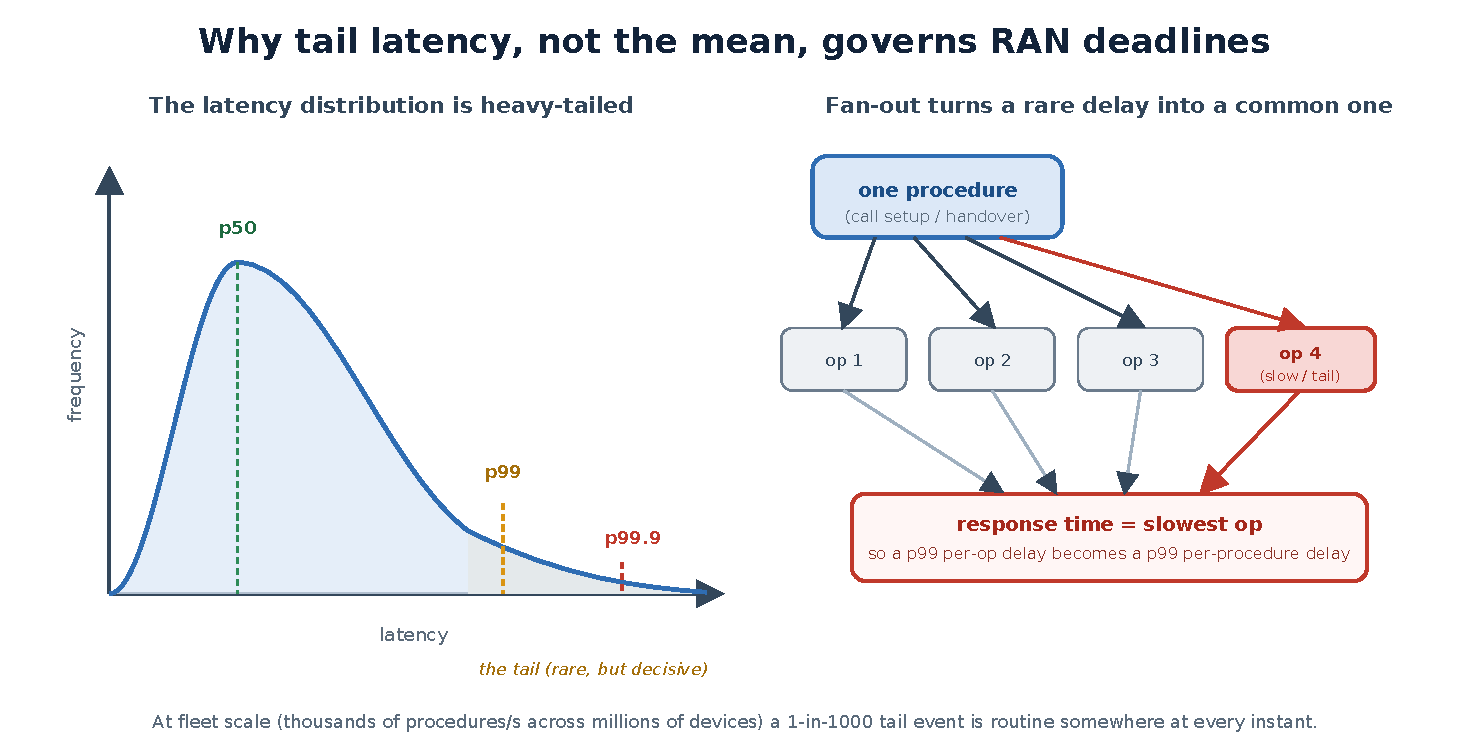
\includegraphics[width=0.78\linewidth]{diagrams/pdf/11_tail_latency_concept.pdf}
\caption[Why the tail, not the mean, governs RAN deadlines]{Why the tail, not the mean, governs RAN deadlines. On the left, most operations
finish quickly and a few take far longer, so the p99 and p99.9 percentiles sit well to the right
of the median. On the right, a procedure such as a call setup runs several operations and
finishes only when the slowest one does, so a delay hitting one operation in a hundred reaches a
much larger share of procedures. At fleet scale a one-in-a-thousand delay is happening somewhere
at every instant.\label{fig:tailconcept}}
\end{figure}

Real-time systems are conventionally graded by the consequence of a missed deadline: in
\emph{hard} real-time a miss is a failure, in \emph{firm} real-time a late result is useless
but not catastrophic, and in \emph{soft} real-time a miss merely degrades quality. A RAN
control plane is best seen as soft-to-firm real-time: an occasional late signalling response
degrades service rather than endangering it, but at fleet scale and under signalling storms
such degradations accumulate into a network-wide reliability problem. This is compounded by
queueing behaviour: as offered load approaches service capacity, queueing delay grows
sharply and the latency tail explodes near saturation. Characterising a system therefore
requires driving it not just at nominal load but \emph{into overload}, which is why the
evaluation in this thesis sweeps load up to and beyond the saturation point.

Measuring tail latency correctly is itself a pitfall. A naive closed-loop load generator
that waits for each response before issuing the next request suffers \emph{coordinated
omission}: when the system stalls, the generator stalls with it and simply fails to record
the many requests that would have arrived during the stall, systematically hiding the very
tail it is meant to expose. Figure~\ref{fig:coord} contrasts the two generator models.
The distinction beneath this is a modelling one, not an
implementation detail. In a closed system a new request is triggered only by the completion of a
previous one, whereas in an open system arrivals are independent of completions, and the two
produce systematically different response-time behaviour on the same service process, with the
closed model reporting the lower figures~\cite{schroeder2006openclosed}. Sound measurement
therefore requires an open-loop model with an
intended schedule, correction for coordinated omission, high-dynamic-range latency histograms
that retain resolution across many orders of magnitude, and statistically rigorous reporting
with repeated runs and confidence intervals rather than single point
estimates~\cite{georges2007rigorous}. These techniques are applied in
Chapter~\ref{chapter:eval}.

\begin{figure}[ht]
\centering
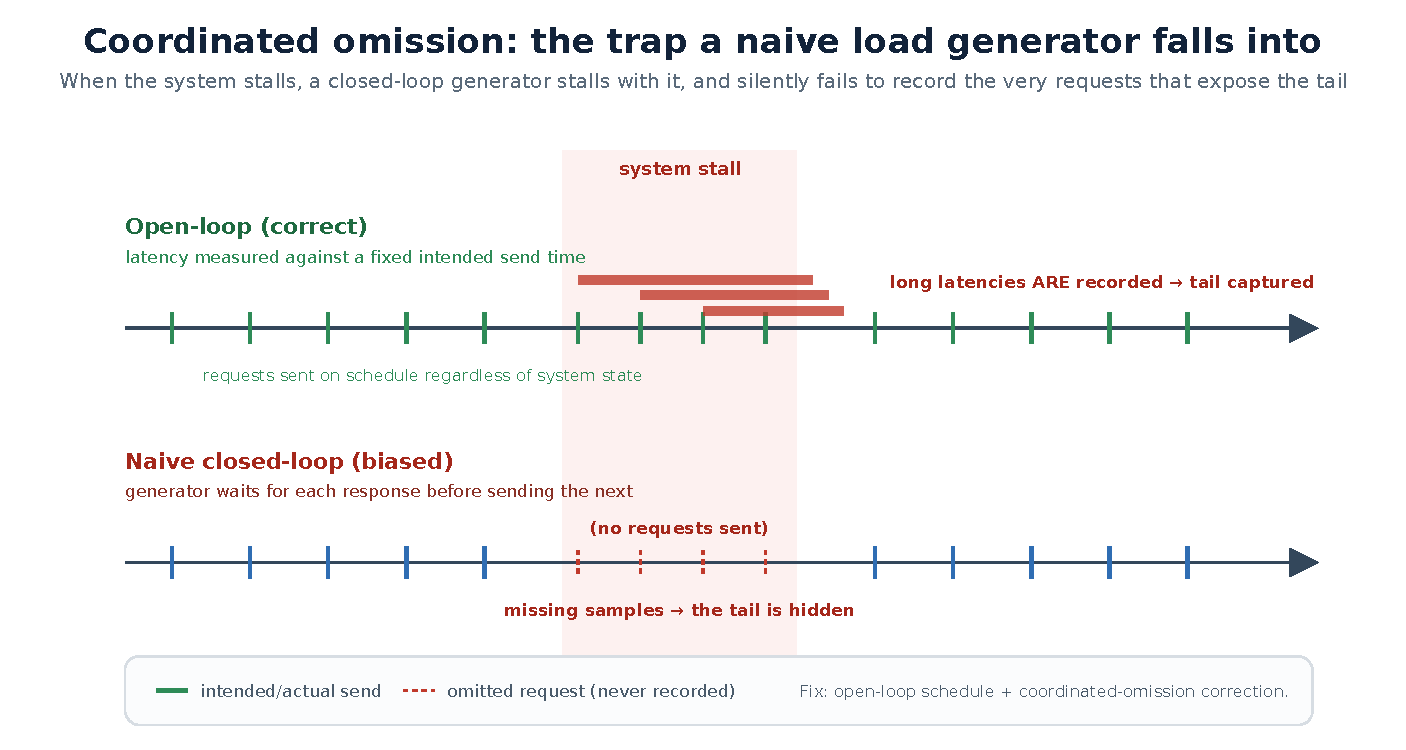
\includegraphics[width=0.78\linewidth]{diagrams/pdf/16_coordinated_omission.pdf}
\caption[Coordinated omission under open- and closed-loop load]{Coordinated omission. The open-loop generator at the top sends on a fixed timetable
even while the system is stalled, and times each request from the moment it was due, so stalled
requests are recorded with their full delay and the tail shows up. The closed-loop generator at
the bottom sends the next request only after the previous reply arrives. When the system stalls
it stops sending too, so the slowest requests are never issued and never measured, and the tail
vanishes from the data.\label{fig:coord}}
\end{figure}

\section{C++ for latency-critical systems}\label{sec:cpplatency}
C++ is the default language for RAN control-plane software for good reasons. It offers
zero-overhead abstractions, direct control over memory layout and allocation, deterministic
destruction through the Resource Acquisition Is Initialization (RAII) idiom, and mature
compilers, libraries, and profiling tools, all without a garbage collector that could inject
unpredictable pauses. Modern C++ (C++11 and later) adds smart pointers
(\texttt{std::unique\_ptr}, \texttt{std::shared\_ptr}) that automate ownership, move semantics
that avoid needless copies, and a formal memory model with \texttt{std::atomic} for
lock-based and lock-free concurrency. These features make it possible to write fast and, with
discipline, reasonably safe systems code.

The difficulty is that the compiler does not enforce this safety. The programmer does. RAII and
smart pointers reduce lifetime errors without eliminating them. A raw pointer or reference can
outlive the object it points to, a container mutation can invalidate an iterator, an object can
be used after it has been moved from, and nothing in the type system stops a mutable object
being shared and written by several threads at once. The result is a familiar catalogue of
defects, use-after-free, double-free, buffer overflow, data races, deadlocks, and iterator
invalidation, that are easy to introduce and expensive to find at telecom scale. Memory-corruption errors of this kind have
been a persistent security problem for decades, and deployed mitigations remain only partial
defences~\cite{szekeres2013sok}. Their prevalence is well documented in
industry. Memory-safety issues account for roughly 70\,\% of the security vulnerabilities
reported at Microsoft~\cite{msrc2019memory}, and Google reports a sharp drop in such
vulnerabilities as memory-safe languages are adopted in Android, to below a fifth of that
platform's total vulnerabilities by
2025~\cite{google2022android,vanderstoep2025android}. This
specific catalogue is developed in detail in Chapter~\ref{chapter:context} and forms the basis
for the fault-injection study in Chapter~\ref{chapter:eval}.

C++ practice mitigates these defects with tooling rather than with language guarantees, and
the tooling is inherently partial. Dynamic sanitisers such as AddressSanitizer (ASan),
ThreadSanitizer (TSan), and UndefinedBehaviorSanitizer detect many errors, but only on the
code paths that a given test actually executes with the right inputs, and they impose runtime
and memory overheads that make them unsuitable for production. TSan in particular reports only
those data races that happen to occur during a run, so a race that manifests only under a rare
interleaving can pass unnoticed. Its deadlock detector inherits that limitation from the technique
it implements, which infers deadlock potentials from the lock-acquisition graph of a single
trace~\cite{bensalem2005deadlock}, and it ships as an experimental component covering only the
POSIX mutex families~\cite{tsandeadlock}. Static analysers help but suffer false negatives and cannot
reason about the whole program. Detection is therefore best-effort and after the fact, which
is precisely the situation a language with compile-time guarantees is meant to change.

That describes C++ as it can be deployed today, and the language is not standing still. Since
2023 the standards committee has pursued \emph{profiles}: named sets of rules covering type,
bounds, lifetime, and arithmetic safety that a conforming implementation must enforce wherever
they are enabled~\cite{sutter2025profiles}. That direction was chosen over \emph{Safe C++}, a
proposal for a safe subset with borrow checking and its own standard library, which is Rust's
model expressed in C++~\cite{baxter2024safecpp}. The comparison drawn here nonetheless stays
live. Profiles are not yet standardised, and in January 2026 their own authors were still
calling for implementations and treating the design of the initial profiles as work still to be
done~\cite{vandevoorde2026profiles}. The concurrency profile, the one that would bear on the
defect classes catalogued in Chapter~\ref{chapter:context}, is placed after that initial set and
not within it: ``more profiles should be defined and implemented, notably a concurrency
profile''~\cite{vandevoorde2026profiles}. A rule enforced only when it is switched on is also a
different kind of thing from a property the type system carries unconditionally, especially
where the enforcement is a run-time check and not a compile-time rejection. The implementations
compared here are therefore built against C++23 as specified and shipped, and
Section~\ref{sec:threats} records what that pins the comparison to.

\section{The Rust ownership and safety model}
Rust enforces memory safety and data-race freedom at compile time through its ownership and
borrowing model~\cite{klabnik2023rust}, and ships with modern tooling in Cargo and integrated
testing. The type system statically forbids mutation of shared state and confines the
unavoidable exceptions to \texttt{unsafe} code kept behind safe APIs~\cite{jung2021safe}.

These guarantees rest on more than assertion. The soundness of the safe fragment of the
language, including the role of \texttt{unsafe} as an explicitly marked escape hatch, has
been established formally by the RustBelt project~\cite{jung2018rustbelt}, and the aliasing
discipline that even \texttt{unsafe} code must respect has been given a precise operational
semantics~\cite{jung2020stacked}. Empirical evidence supports the model in practice: in real
codebases \texttt{unsafe} is used sparingly and in localised
ways~\cite{qin2020rust,astrauskas2020unsafe}, and a study of all Rust memory-safety CVEs found
that every one of them but a single compiler bug involved \texttt{unsafe}
code~\cite{xu2021rustcve}. The caveat is that unsafety propagates through dependencies. Fewer
than a third of libraries use \texttt{unsafe} directly, but a much larger fraction cannot be
fully statically checked because it hides somewhere in their call
chain~\cite{evans2020rust}, which is a further argument for keeping the safety-critical core of a
subsystem \texttt{unsafe}-free, as this thesis does.

One property matters most in a latency-critical setting. This safety comes from the type system
and the borrow checker, not from runtime instrumentation, and is intended to be
\emph{zero-cost}. Systems research argues Rust attains safety without the overhead of garbage
collection or runtime checks, and even enables efficiency techniques that are impractical in
C~\cite{balasubramanian2017rust}. Whether that zero-cost claim holds for a telecom
control-plane workload is precisely the property this thesis evaluates.

Concretely, the borrow checker rejects at compile time the very use-after-free sketched in the
introduction: a program that frees a context while a reference to it is still live does not
build. Figure~\ref{fig:borrowuaf} puts that defect in its UE Context Management form beside the
C++ version, which compiles and is caught, if at all, only at runtime.

\begin{figure}[ht]
\centering
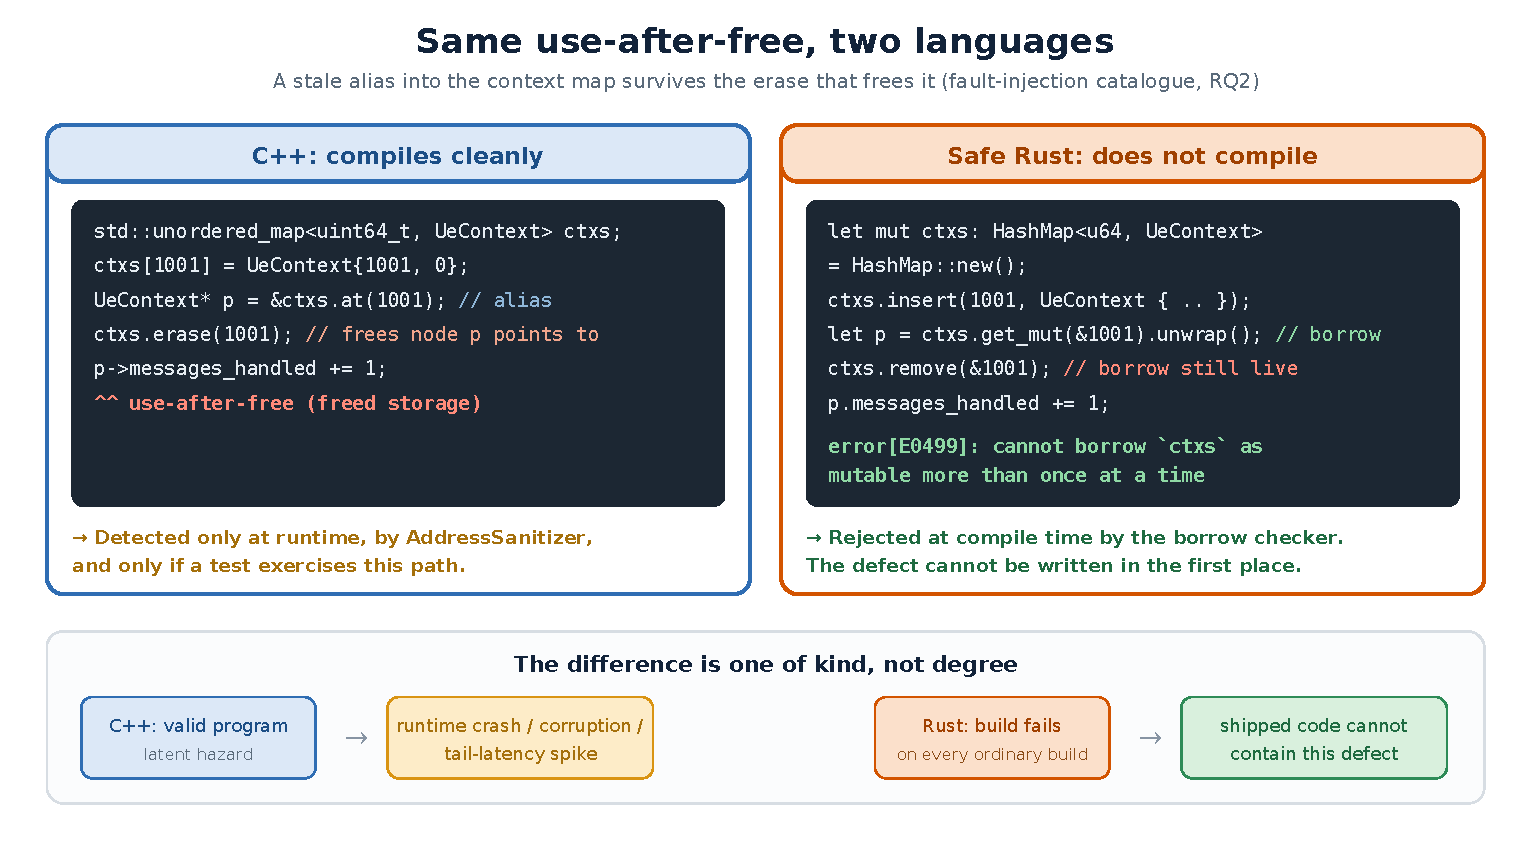
\includegraphics[width=0.78\linewidth]{diagrams/pdf/08_borrow_checker_uaf.pdf}
\caption[The same use-after-free in C++ and in safe Rust]{The same use-after-free defect in C++ and in safe Rust. The stale alias into the
context map survives the \texttt{erase}/\texttt{remove} that frees it: in C++ this compiles and
is caught only at runtime, and only under a sanitiser on a path a test exercises, whereas
in safe Rust the borrow checker rejects it at compile time (\texttt{E0499}), so the defect
cannot be written at all. The difference is one of kind, not degree.\label{fig:borrowuaf}}
\end{figure}

The same discipline extends to concurrency. Rust encodes thread-safety in the type
system through the \texttt{Send} and \texttt{Sync} marker traits: a value may cross a thread
boundary only if its type is \texttt{Send}, and may be shared by reference across threads only
if it is \texttt{Sync}. Sharing a value that permits unsynchronised mutation is therefore a
compile error, not a latent race. This is the property Rust markets as ``fearless concurrency.''
Error handling is likewise explicit: fallible operations return a \texttt{Result} value that
the caller must handle, rather than raising an exception that unwinds through hidden control
flow. Both the cost and the control flow of the failure path therefore stay visible, which is
an advantage in latency-sensitive code where surprises in the tail are what matter.

Rust is not the only memory-safe language, and the reason the comparison here is drawn against
C++ rather than against a managed runtime belongs with this model. Java, C\# and Go achieve
memory safety through a runtime and garbage collection, which is an excellent trade for much
software and a poor one for a tail-latency-critical control plane: collection pauses are a
recognised source of tail latency in large systems~\cite{dean2013tail}, and a managed runtime
gives up the control over memory layout and scheduling this domain relies on. C, at the other
extreme, is as memory-unsafe as C++ while offering fewer abstractions for building large
systems. Rust is the first widely supported language to combine compile-time memory and thread
safety with the absence of a garbage collector and throughput and memory use alongside C and
C++~\cite{balasubramanian2017rust,jung2021safe,bugden2022rust}. That is why managed languages
are out of scope and why the meaningful comparison for RAN control-plane software is C++ against
Rust.

Table~\ref{tab:langmodel} sets the two languages' mechanisms side by side. The distinction it
is built around is not which hazards each language names, since both name much the same ones,
but \emph{when} and \emph{by what} each is ruled out, and the last two rows mark where the
answer stops being ``by the compiler'' for either of them.

\begin{table}[H]
\centering
\small
\caption[How each language enforces the properties measured here]{How each language enforces the properties this thesis measures. The rows above the
rule are the ones on which the two differ in kind rather than in degree: a compiler that
rejects a program rules the defect out of every execution of it, whereas a sanitiser rules it
out only of the executions an instrumented test happens to take. The rows below the rule are
the boundary developed in Chapter~\ref{chapter:context} and measured in
Chapter~\ref{chapter:eval}, where neither language offers a static
guarantee.\label{tab:langmodel}}
\renewcommand{\arraystretch}{1.2}
\begin{tabular}{@{}R{0.20\linewidth} R{0.36\linewidth} R{0.36\linewidth}@{}}
\hline\hline
Concern & Modern C++ & Rust \\
\hline
Object lifetime & RAII and smart pointers, applied by convention. A raw pointer or reference may outlive its referent & Ownership: each value has one owner and is dropped exactly once \\
Aliasing & Unrestricted: any number of mutable aliases may coexist & Borrowing: either one mutable reference or many shared ones, never both \\
Bounds & Unchecked on \texttt{operator[]}, checked only through \texttt{at()} & Checked by default, elided where the index can be proved in range \\
Thread safety & Not expressed in the type system: sharing a mutable object across threads compiles & \texttt{Send} and \texttt{Sync} marker traits. Unsynchronised sharing is a type error \\
Error signalling & Exceptions or error codes: the failure path can be invisible at the call site & \texttt{Result} values the caller must handle. The failure path is explicit \\
Escape hatch & The whole language & \texttt{unsafe} blocks, delimited and mechanically countable \\
Stage of detection & Run time, under the right sanitiser, on a path a test exercises & Compile time, on every ordinary build, whatever the test coverage \\
\hline
Lock-acquisition order & Not checked & Not checked \\
Atomicity of a composed operation & Not checked & Not checked \\
\hline
\end{tabular}
\end{table}

\section{Concurrency models for control-plane software}
How concurrency is structured shapes both correctness and tail latency. The dominant model is
\emph{shared-memory} concurrency, in which threads mutate common state guarded by mutexes and
atomics. It is flexible, but it is the source of races, deadlocks, lock contention, and priority
inversion, and its worst case is hard to bound. The alternative is \emph{message-passing} or
\emph{shared-nothing} concurrency, in which state is partitioned so that each piece is owned by
a single thread and all interaction happens through messages, as in the actor model. It trades
flexibility for scalability and much simpler reasoning, and it maps onto per-UE partitioning
naturally, since each UE's state is largely independent. The choice also moves the quantity
measured here: thread-per-core structuring changes application tail latency on its
own~\cite{enberg2019threadpercore}, so the model is held fixed across both implementations
instead of left to each language's idiom. Figure~\ref{fig:concmodels} contrasts the two.

\begin{figure}[ht]
\centering
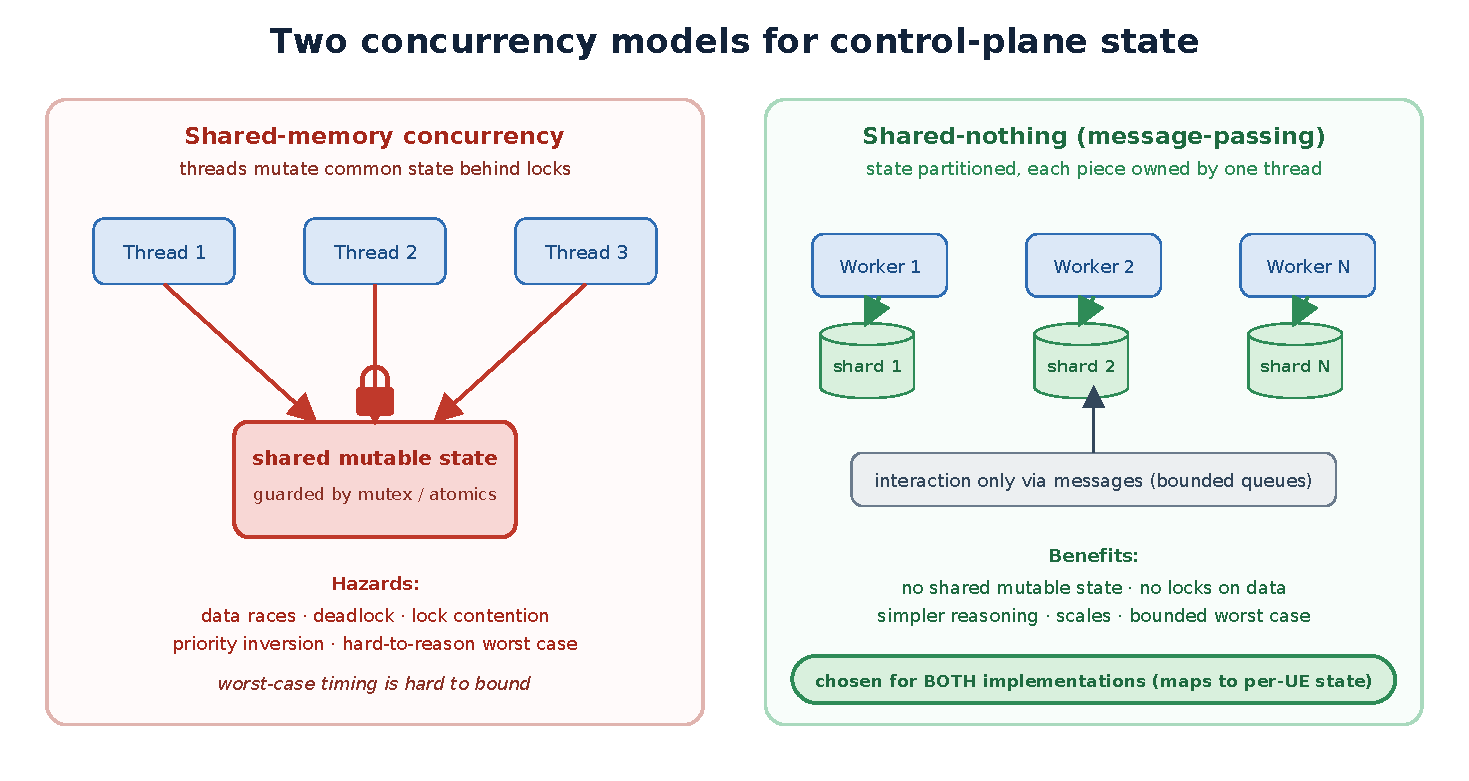
\includegraphics[width=0.78\linewidth]{diagrams/pdf/12_concurrency_models.pdf}
\caption[Two concurrency models for control-plane state]{Two concurrency models for control-plane state. Shared-memory concurrency (left) lets
threads mutate common state behind locks and is the source of data races, deadlock, and lock
contention, with a worst case that is hard to bound. Shared-nothing message-passing (right)
partitions state so each shard is owned by a single worker and all interaction goes through
bounded queues, which removes locks on context data and maps onto per-UE partitioning. It is the
model adopted for both implementations.\label{fig:concmodels}}
\end{figure}

A third structure, an asynchronous runtime over a work-stealing scheduler, is idiomatic in both
languages and used in neither. Its timing behaviour belongs to the runtime, not to the language
hosting it: a real-time study of asynchronous Rust finds one application meeting or missing its
deadlines depending on the runtime and thread-priority mapping it is given, and the configuration
that meets them is not the idiomatic work-stealing one~\cite{skoudlil2025asyncrust}. Adopting such
a runtime would import the variable this study exists to exclude, and
Section~\ref{sec:relatedwork} returns to a comparison in which it was not excluded.

Queueing between producers and consumers is a second, independent choice. Unbounded queues mask
overload and let latency and memory grow without limit. \emph{Bounded} queues, whether they block
for backpressure or shed, bound worst-case memory and make overload visible, which predictable
tail latency requires. Both choices fix the architecture used by both implementations in
Chapter~\ref{chapter:design}: a shared-nothing, thread-per-shard design in which UE state is
divided into independent slices
called \emph{shards}, each owned by exactly one worker thread, so no two threads ever touch the
same context. Requests reach a shard through a bounded multi-producer, single-consumer queue that
blocks when full.

\section{Interoperability between C++ and Rust}\label{sec:interop}
Adopting a new language in a large existing system is necessarily incremental: a Rust component
must coexist with and be callable from a substantial C++ codebase. The common denominator for
that is the C application binary interface (ABI). Rust can expose functions with
\texttt{extern "C"} linkage and hand out \emph{opaque handles} to Rust-owned objects, which C++
calls through a C header. Tooling automates parts of this: \texttt{bindgen} (Rust bindings from
C headers), \texttt{cbindgen} (C headers from Rust), and the \texttt{cxx} crate (a safer
bidirectional bridge). Interoperability is not free. Crossing the boundary steps outside the
checked language, so the seam must contain \texttt{unsafe} code, values beyond the simplest need
marshalling, and the foreign interface has to be designed deliberately. Seam size, the
\texttt{unsafe} it concentrates, and per-call crossing cost are the quantities RQ4 measures in
Chapter~\ref{chapter:eval}.

One distinction bounds what those measurements can establish. Concentrating \texttt{unsafe} in
the seam says what the compiler checks, not what can happen at run time. A Rust component linked
into a C++ host shares one address space with it, so a defect on the C++ side can corrupt
Rust-owned data however much of the Rust side the borrow checker verified. This has been shown
experimentally, and the proposed remedies isolate the two heaps in hardware or in the runtime
instead of trusting the discipline of the
interface~\cite{rivera2021galeed,kirth2022pkrusafe}. The defect classes specific to Rust/C
boundaries have been catalogued separately from those of either
language~\cite{li2022crosslang}, and the binding generators themselves carry
bugs~\cite{cai2026interop}. The consequence is stated once here and honoured throughout: an
\texttt{unsafe}-free core means the core's own defects are ruled out at compile time, and it
does not mean the core is protected from its host.

What has moved recently is the reach of the tooling, not the guarantee. A stateless model
checker for Rust now explores the state space of a program together with its foreign
dependencies, which puts data races arising from the interaction of the two languages within
reach of a checker even though they sit outside what the borrow checker
sees~\cite{pearce2026rustmc}. That capability arrived after the prototype measured here was
built, and Chapter~\ref{chapter:conclusions} records it as the next step for the seam.

\section{Research gap}\label{sec:gap}
The preceding sections set up the gap. The RAN control plane is a soft-to-firm real-time,
highly concurrent domain where tail behaviour under overload, not average throughput, governs
the quality the network delivers. C++ supplies the control and performance the domain demands,
but leaves whole classes of memory and concurrency defects to best-effort detection after the
fact. Rust promises to prevent those classes at compile time at no run-time cost, and offers a
credible incremental adoption path through the C ABI.

The domain is not unstudied, and the volume of prior work is easy to underestimate because
almost none of it is indexed. At least five vendor-hosted master's theses, all carried out at
Ericsson, have compared candidate languages for RAN and telecom software. One weighs runtime
cost against development efficiency across C++, Rust, and Go~\cite{karlback2021ran}. One asks
whether Rust could replace C in RAN node management~\cite{olsson2023ranmgmt}. One builds a
thread-per-core packet processor on asynchronous Rust and measures it against the DPDK
application it mirrors~\cite{olsson2023asyncpackets}. One measures median and 99th-percentile
latency for control-plane procedures across five asynchronous programming
frameworks~\cite{arvidsson2025async}. The last builds matched C++ and Rust implementations of an
ASN.1 decompiler and compares them statistically~\cite{emberg2023asn1}. All five are directly
relevant, and two report differences unfavourable to Rust.

Three of them vary the language together with the runtime and the concurrency model, so a
measured difference cannot be attributed to the language rather than to the framework built on
it~\cite{karlback2021ran,olsson2023asyncpackets,arvidsson2025async}. The effect sizes reach a
factor of five, which is an indication of how much of the measurement the runtime owns. The
remaining two hold the design closer to fixed but report execution time and peak memory rather
than tail behaviour under rising load~\cite{olsson2023ranmgmt,emberg2023asn1}, and the closest
of them, Emberg and Wadsten, measures a stateless transformation rather than a stateful,
concurrent subsystem. Figure~\ref{fig:gapmap} sets the neighbouring studies against the
properties a controlled answer would require, and the pattern it shows is that each holds some
of them and none holds all.

The concentration of that evidence is itself part of the gap. All five studies come from one
vendor, and their conclusions have never been tested against another organisation's software,
targets or conventions, so what is known about this question is what one company's frameworks
report about it. The published record on the other side is emptier: there is no study of Rust
among the indexed publications of the vendor hosting this work, and the nearest peer-reviewed
position from that side argues for making memory-error sanitisation practical rather than for
replacing it with a compile-time guarantee~\cite{gjomemo2016mesc}, which is the strategy this
thesis tests against. Section~\ref{sec:relatedwork} compares the five with this study directly.

\begin{figure}[ht]
\centering
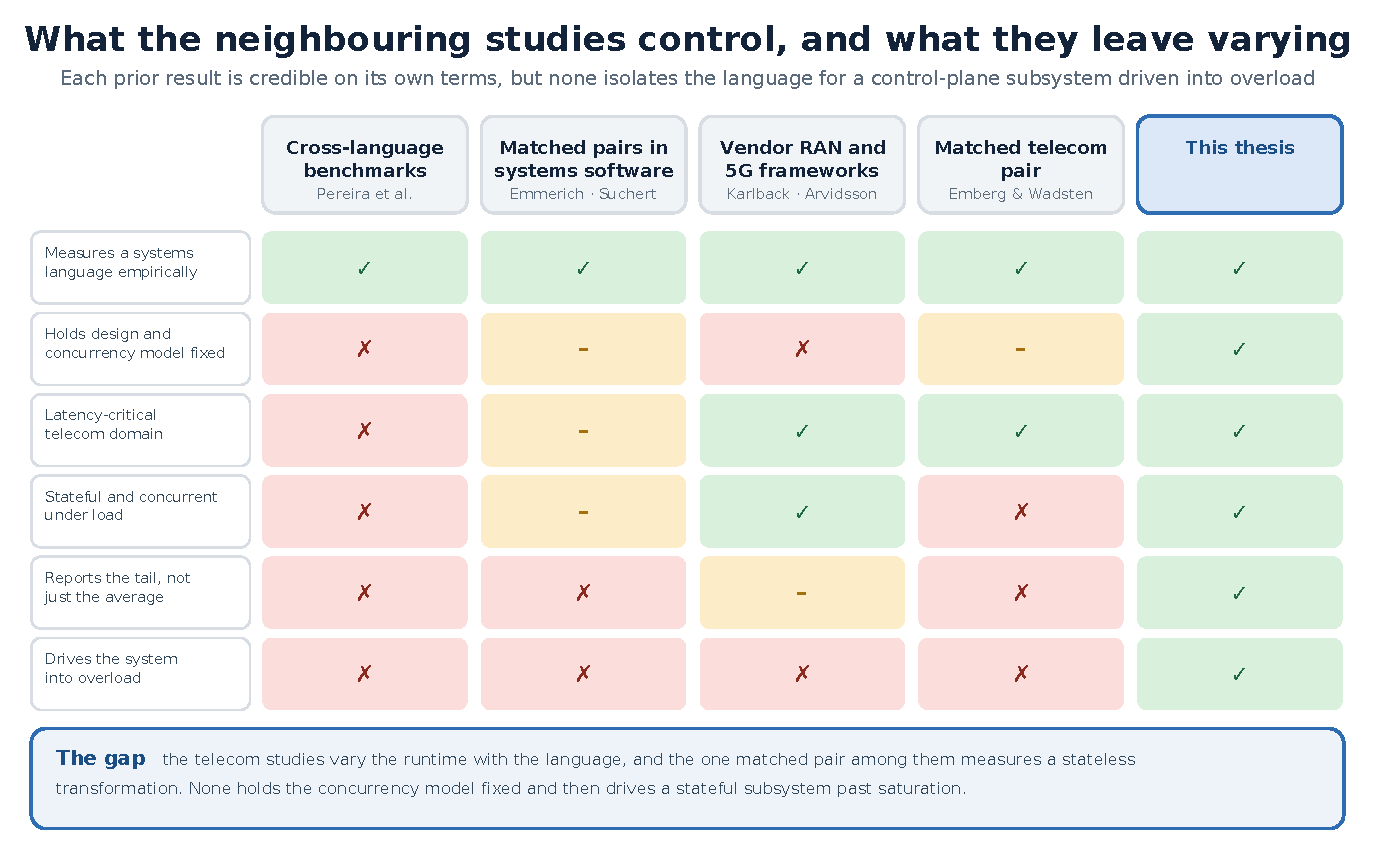
\includegraphics[width=0.78\linewidth]{diagrams/pdf/29_research_gap.pdf}
\caption[What the neighbouring studies control, and what they leave varying]{What the neighbouring studies control, and what they leave varying. Each row is a
property that a controlled answer to the research questions would need. Each column is a study.
The general cross-language comparisons measure the right kind of object but the wrong regime,
reporting averages on general-purpose workloads. Matched pairs in systems software hold the
design fixed, but outside this domain and below saturation. The vendor RAN and 5G framework
studies reach the right domain, and one of them reports the tail, but in all of them the
language varies together with the runtime and the concurrency model. The one matched telecom
pair, Emberg and Wadsten, controls the design but measures a stateless transformation. Holding
the design and the concurrency model fixed for a stateful, concurrent subsystem and then driving
it past saturation is what this thesis adds. The contribution is the control, not a new
measurement technique.\label{fig:gapmap}}
\end{figure}

What is therefore missing from the literature
is \emph{direct, controlled} evidence for a representative control-plane subsystem: whether
Rust actually holds its tail latency and predictability under overload against modern C++
\emph{when the concurrency model, algorithms, and data structures are held fixed},
exactly which defect classes it eliminates and at what stage the remainder are caught, what
its safety model costs in throughput and resources, and what incremental adoption costs in
practice. Closing this gap is the purpose of the four research questions. The next chapter
grounds them in the specific subsystem, defect classes, and timing properties at stake, and
Chapter~\ref{chapter:methodology} sets out the methodology by which they are pursued.

\chapter{Problem Context: UE Context Management and Predictability\label{chapter:context}}
\chaptermark{Problem Context}

\section{The UE Context Management subsystem}\label{sec:uecm}
The subsystem under study is a UE Context Management service. It is modelled on a real Nokia
gNB-CU-CP service domain that owns the UE context lifecycle, RRC procedure
execution~\cite{3gpp38331}, and mobility/handover, which are the functions the 3GPP architecture
assigns to the control-plane part of a disaggregated gNB (Section~\ref{sec:ranarch}).

Figure~\ref{fig:fsm} shows the UE-context lifecycle state machine that both implementations
encode identically. This state machine is exactly what the mixed workload
of Section~\ref{sec:workload} walks each UE through.

\begin{figure}[ht]
\centering
\begin{tikzpicture}[
    ->, >=Stealth, node distance=3.2cm, font=\small,
    every state/.style={draw, minimum size=1.5cm, fill=blue!6, thick},
    every edge/.style={draw, thick}
  ]
  \node[state, initial, initial text=\scriptsize create] (idle) {Idle};
  \node[state, right=of idle] (conn) {Connected};
  \node[state, right=of conn] (reconf) {Reconf.};
  \node[state, below=1.9cm of conn, fill=gray!10] (rel) {Released};

  \path (idle)  edge node[above,font=\scriptsize]{setup} (conn)
        (conn)  edge[bend left=18] node[above,font=\scriptsize]{begin} (reconf)
        (reconf) edge[bend left=18] node[below,font=\scriptsize]{complete / abort} (conn)
        (conn)  edge node[right,font=\scriptsize,pos=0.45]{release} (rel)
        (idle)  edge[bend right=32] node[below,font=\scriptsize,pos=0.6]{release} (rel);
  \path (conn) edge[loop above] node[font=\scriptsize]{signal / add\_drb} (conn);
\end{tikzpicture}
\caption[UE-context lifecycle state machine]{UE-context lifecycle state machine. \texttt{create} allocates a context in
\texttt{Idle} and \texttt{setup} connects it. \texttt{signal} and \texttt{add\_drb} are handled
in place while \texttt{Connected}. A reconfiguration or handover moves through
\texttt{Reconfiguring} and back on \texttt{complete} or \texttt{abort}, and \texttt{release}
tears the context down. Operations invalid for the current state return an \texttt{OpError}
instead of changing state.\label{fig:fsm}}
\end{figure}

\paragraph{Why this subsystem.}
UECM works as a study object because it is both representative and small enough to control. It
is core RAN layer-3 functionality, and it carries the properties that make production
control-plane code difficult: per-UE mutable state, a strict operation lifecycle, high
concurrency across UEs, and the latency and reliability targets the 5G system sets for
control-plane procedures~\cite{3gpp38913,3gpp22261}. Conclusions about how a language handles
those properties therefore transfer to other stateful, concurrent control-plane services. The
subsystem is also small enough to specify precisely, implement faithfully in two languages, and
reason about in full, which is what makes a parity-tested comparison possible at all. A larger
subsystem would buy external validity at the cost of the internal validity a fair language
comparison depends on. UECM sits where both stay within reach.

\paragraph{Operation set.}
The interface exercised by the study is deliberately small and lifecycle-oriented. It can create
and release a context, set up a connection (\texttt{Idle}$\rightarrow$\texttt{Connected}), handle
an in-session signalling message, add a data radio bearer, begin, complete, or abort a
reconfiguration or handover, and look up a context's state under concurrent load. Every operation is
defined for every state of the machine in Figure~\ref{fig:fsm}: an operation that is illegal in
the current state returns a typed error and leaves the context unchanged, rather than throwing
or corrupting state. This closed, well-typed operation set is what lets the same test vectors
and the same workload drive both implementations along identical paths
(Section~\ref{sec:parity}).

\section{Memory-safety and concurrency defect classes}\label{sec:defects}
The defects that affect C++ control-plane code of this kind fall into two families. The
\emph{memory-safety} family concerns the lifetime and bounds of objects: a \emph{use-after-free}
accesses storage that has already been released, a \emph{double-free} releases the same storage
twice, and a \emph{buffer overflow} reads or writes past the end of an allocation. The
\emph{concurrency} family concerns unsynchronised or ill-ordered access from multiple threads: a
\emph{data race} is a pair of unsynchronised accesses to the same location of which at least one
is a write, a \emph{deadlock} is a cyclic wait for locks, and \emph{iterator invalidation} is
the use of an iterator or reference into a container after a mutation has moved or freed the
underlying storage. What these share is that they are all \emph{silent} in C++: each is accepted
by the compiler and, on the paths ordinary tests happen to exercise, may appear to work,
surfacing only later as corruption, a crash, or an unpredictable latency spike. These are the
same memory-corruption classes that decades of security research have struggled to contain in C
and C++~\cite{szekeres2013sok}.

Each class has a natural incarnation in UE Context Management, which is why the subsystem is a
good vehicle for studying them:

\begin{itemize}
  \item \textbf{Use-after-free.} A signalling message holds a raw pointer or reference to a UE
        context that a concurrent \texttt{release} has already erased from the context map. The
        in-flight handler then dereferences freed storage.
  \item \textbf{Double-free.} A release path runs twice for the same UE, for example because a
        retransmitted release is not made idempotent, freeing the context's owned resources a
        second time.
  \item \textbf{Iterator invalidation.} Code iterates a context's data-radio-bearer list while
        adding or removing a bearer, so the iterator refers into storage the container has since
        reallocated.
  \item \textbf{Data race.} Two workers update the same context field, an activity counter or a
        state flag, without synchronisation, so the accesses race.
  \item \textbf{Unguarded shared mutation.} A context is shared by reference across threads and
        mutated without a lock or other discipline, a race whose root cause is the absence of any
        ownership rule for the shared state.
  \item \textbf{Use-after-move.} Admission moves a freshly built context into the store and
        then answers the request from the local variable it has just moved from, so the
        acknowledgement carries an empty identity. This class is carried for what the C++
        tooling does \emph{not} say about it. Nothing is corrupted and nothing is undefined,
        because a moved-from object is in a valid but unspecified state, so the defect has no
        runtime symptom for a sanitiser to find.
  \item \textbf{Thread-unsafe handle shared across workers.} A refcounted context handle whose
        counter is not atomic, the idiom a hot path reaches for when the atomic control block of
        a shared pointer costs more than it is worth, is passed to two shard workers. The
        constraint that makes the handle correct is written in a comment, because C++ has no way
        to state thread affinity in a type.
\end{itemize}

These seven classes lie squarely within the guarantees Rust claims to provide, which makes them
the natural test of whether that claim holds. Testing only them, however, would build the
expected answer into the choice of test cases, so seven further classes are carried into the
study for the opposite reason, because there is good reason to expect that safe Rust does
\emph{not} prevent them:

\begin{itemize}
  \item \textbf{Lock-order deadlock.} A handover locks the source UE context and then the
        target while a concurrent handover in the opposite direction locks target then source,
        and the two wait for each other indefinitely. Nothing about object lifetimes or
        aliasing is violated. The fault is in the order of acquisition.
  \item \textbf{Lost update.} Two workers increment a context's activity counter through a
        read-modify-write split across two separate critical sections. Every individual access
        is correctly synchronised, so this is a \emph{race condition} rather than a
        \emph{data race}: the atomicity violation lives in the composition of the operations,
        not in the memory accesses themselves, and it corrupts a value silently instead of
        crashing.
  \item \textbf{Leak through a reference cycle.} A context and the peer it is being handed
        over to hold owning references to each other, so neither reference count reaches zero
        and neither is ever destroyed. Reference counting cannot collect a cycle in either
        language, and leaking is safe in Rust by explicit design. This is the cleanest
        statement of a boundary in the catalogue, because both languages fail identically.
  \item \textbf{Integer overflow in a release build.} A bearer's TEID stride computation
        exceeds the width of its type. In C++ signed overflow is \emph{undefined}, so the
        program has no meaning. In Rust it is \emph{defined} to wrap, because the
        \texttt{opt-level~=~2} profile this study compares leaves \texttt{overflow-checks}
        off, so the program has a meaning and the meaning is wrong. The pattern is not
        hypothetical: CVE-2026-64467 in \texttt{rust\_binder} is a stride error of this shape.
  \item \textbf{Worker failure blast radius.} One shard worker fails part-way through a
        procedure. The concurrency model of Section~\ref{sec:concurrency} makes a shard
        a failure domain by construction, and neither language's type system enforces that it
        behaves as one: in C++ an exception escaping the thread callable terminates the whole
        process, and in Rust the panic is confined to its thread but poisons the state it held,
        so the damage propagates along the data instead. Directly relevant to a carrier-grade
        availability argument, and addressed by nothing in either type system.
  \item \textbf{Double-free across the seam.} A C++ host holds an opaque handle to a Rust
        context and releases it twice, which is the retransmitted release of the double-free
        class above, now expressed the way a foreign-function boundary has to express it. Safe
        Rust rejects the double release because ownership tracks the value. A seam cannot keep
        that, since handing a raw pointer to a C caller is exactly the operation that ends the
        compiler's knowledge of it. The class therefore appears on both sides of the boundary,
        which is the sharpest available statement of what the boundary is.
  \item \textbf{Forgotten lock guard.} Bearer setup takes the context lock and a validation
        failure returns without releasing it, so the next worker to touch that context waits
        indefinitely. Rust removes the ordinary form of this bug, because a guard releases when
        it is dropped and there is no hand-written unlock to skip. It does not remove the bug,
        because a guard is a value and leaking a value is safe. Where the reference cycle leaks
        memory, this leaks the context itself.
\end{itemize}

Together these fourteen form the catalogue injected in Chapter~\ref{chapter:eval}, and the
split between the two groups is what lets the study report a boundary rather than a verdict.
Buffer overflow is described above for completeness but is not injected, because neither
implementation performs raw pointer arithmetic on the context store, so an injected instance
would be an artificial construct and not a plausible bug in this subsystem.
Table~\ref{tab:defectmap} collects the catalogue with the outcome expected of each case
\emph{before} the study was run, which is the form in which the runner records it: an
expectation written down in advance can be violated in either direction and reported as a
discrepancy, whereas one formed after the fact cannot.

\begin{table}[H]
\centering
\small
\caption[The injected catalogue and its incarnations in UECM]{The injected defect catalogue: each class in the form it would plausibly take in UE
Context Management, and the outcome recorded for it in advance of the study. The last column
is a prediction rather than a result. Table~\ref{tab:taxonomy} reports what was measured, and
the fault runner flags a mismatch in either direction instead of absorbing it into the
conclusion. Buffer overflow is listed for completeness and not injected: neither
implementation does pointer arithmetic on the context store.\label{tab:defectmap}}
\footnotesize
\renewcommand{\arraystretch}{0.95}
\begin{tabular}{@{}R{0.19\linewidth} R{0.40\linewidth} R{0.14\linewidth} R{0.16\linewidth}@{}}
\hline\hline
Defect class & Incarnation in UE Context Management & How it fails & Expected in safe Rust \\
\hline
\multicolumn{4}{@{}l}{\emph{Memory-safety family: object lifetime and bounds}} \\
Use-after-free & An in-flight signalling handler dereferences a context that a concurrent \texttt{release} has already erased from the map & Corruption or crash & Prevented \\
Double-free & A retransmitted release is not made idempotent, so the release path frees the context's resources a second time & Corruption or crash & Prevented \\
Use-after-move & Admission answers the request from the context it has just moved into the store & Silently empty identity & Prevented \\
Buffer overflow & No plausible incarnation here: the context store is reached only through container APIs & n/a & Not injected \\
\hline
\multicolumn{4}{@{}l}{\emph{Concurrency family: unsynchronised or ill-ordered access}} \\
Iterator invalidation & A bearer is added while the context's data-radio-bearer list is being iterated & Corruption or crash & Prevented \\
Data race & Two workers update the same context field, a counter or a state flag, without synchronisation & Torn or lost value & Prevented \\
Unguarded shared mutation & A context is shared across threads and mutated with no ownership rule governing it & Torn or lost value & Prevented \\
Thread-unsafe handle shared & A context handle whose refcount is not atomic is passed to two shard workers & Corrupted refcount & Prevented \\
\hline
\multicolumn{4}{@{}l}{\emph{Boundary group: included because safe Rust is expected \emph{not} to prevent them}} \\
Lock-order deadlock & Opposing handovers lock source-then-target and target-then-source & Hang & Not prevented \\
Lost update & A counter's read-modify-write is split across two critical sections, so each access is synchronised but their composition is not atomic & Silently wrong value & Not prevented \\
Reference-cycle leak & A context and its handover peer hold owning references to each other, so neither reference count reaches zero & Unbounded growth & Not prevented \\
Integer overflow (release build) & A bearer's TEID stride computation exceeds the width of its type & Silently wrong value & Not prevented \\
Worker-failure blast radius & One shard worker fails part-way through a procedure while holding shard state & Outage beyond one shard & Not prevented \\
Double-free across the seam & A C++ host releases an opaque handle to a Rust context twice & Corruption or crash & Not prevented \\
Forgotten lock guard & Bearer setup returns on a validation failure without releasing the context lock & Hang & Not prevented \\
\hline
\end{tabular}
\end{table}

\section{Tail latency and predictability in RAN}
Section~\ref{sec:predictability} set out why the tail rather than the mean governs a
latency-critical system, and what measuring it correctly demands. What that section left
general, this one makes specific, because two properties of the RAN setting are what turn a
methodological preference into the governing metric.

Those properties are fan-out and scale, drawn in Figure~\ref{fig:tailconcept}. One user-visible
action, a call setup or a handover, becomes many dependent control-plane operations whose
slowest member gates completion, and a busy site drives thousands of such procedures per second
across millions of connected devices. Put together, the p99.9 of a single UE Context Management
operation is not a curiosity at the margin of a distribution. It is a rate of degraded
procedures the network sustains continuously.

The scale at which those percentiles matter is not hypothetical. A measurement study of a
disaggregated 5G RAN times the CU-CP-to-DU UE Context Setup procedure over F1-C, and the
CU-CP-to-CU-UP bearer context setup over E1, under different interface-protection schemes, and
finds the choice worth hundreds of microseconds: on F1-C, IPsec adds on the order of
$120\,\mu$s on average to UE context setup, against roughly $430\,\mu$s for
DTLS~\cite{michaelides2026ranlatency}. Overheads of that size are treated as consequential for
precisely the procedure family this thesis reimplements, which places these operations in a
regime where tens of microseconds are an engineering quantity rather than noise.

The study therefore characterises the full latency distribution, focusing on the high
percentiles (p99 and p99.9) and the maximum, and on how these degrade as offered
load approaches and then exceeds saturation (Chapter~\ref{chapter:eval}). Stopping at nominal
load would miss the regime that decides service quality, since queueing delay grows
super-linearly near capacity. It is also the regime in which a difference between two
implementations of one design, if there is one, has room to become visible.

\begin{figure}[ht]
\centering
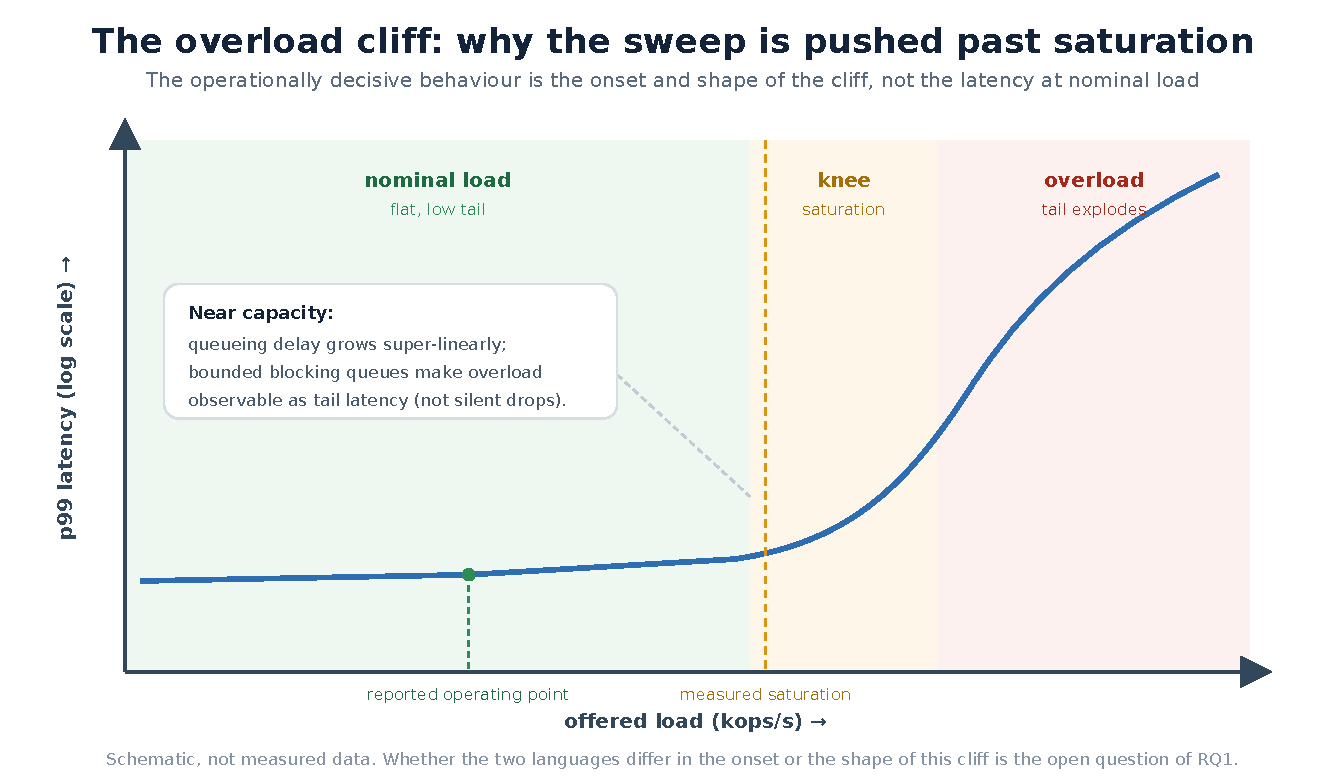
\includegraphics[width=0.70\linewidth]{diagrams/pdf/15_overload_cliff.pdf}
\caption[The overload cliff]{The overload cliff. Tail latency stays low and flat while offered load is below
service capacity, then climbs steeply once the system is driven past saturation and requests
queue behind the bounded, blocking queues. The operationally decisive behaviour is the onset and
shape of this cliff, which is why the load sweep is pushed beyond the saturation point rather
than stopping at nominal load. The figure is a schematic of the phenomenon and not a plot of
this study's data: whether the two languages differ in where the cliff begins or how steeply it
rises is exactly what RQ1 asks, and Section~\ref{sec:overload} reports that they differ in
both.\label{fig:cliff}}
\end{figure}

\chapter{Research Methodology\label{chapter:methodology}}

The previous chapter set out what the study must achieve. This one sets out how. It states
the overall research strategy, the method chosen for each research question and why it is
appropriate, the controls that make a language comparison fair, the statistical treatment of
the measurements, and the reproducibility and ethical commitments under which the work is
carried out.

\section{Research approach}\label{sec:approach}
The study is experimental with a constructive (design-science) element. The artifact is a pair
of functionally equivalent implementations of the subsystem, one in C++ and one in Rust, plus
the framework that benchmarks them. Both are built from a single frozen specification and then
evaluated under controlled experiments. Evidence is triangulated across three methods.
Performance measurement under a load sweep answers RQ1 and RQ3, a controlled fault-injection
study answers RQ2, and an FFI migration case study, part measured and part qualitative, answers
RQ4. The three are independent. A weakness in one of them, such as the environment sensitivity
of tail-latency measurement, therefore does not carry into the conclusions as a whole. Every
measurement reports variance over repeated runs, and Section~\ref{sec:controls} sets out the
controls that keep the language the only variable.

That design follows from the shape of the questions. Each asks how one outcome (tail latency,
defects prevented, resource use, migration cost) depends on one variable, the implementation
language. The language therefore has to be the only systematic difference between the two
objects under test. This rules out the commonest form of language comparison in the literature,
where two independently written programs are measured and the gap is attributed to the language.
Such a gap also carries the design, the libraries and the skill of their authors.

Building both sides from one specification removes that confound. The comparison is then between
two encodings of the same design, and the artifact becomes both the contribution and the
instrument that measures it. Where a question can be answered with numbers, the treatment is
quantitative. Where it cannot, as with the kind of guarantee in RQ2 and the API-design effort in
RQ4, it is qualitative but still systematic.

The gap this design addresses (Section~\ref{sec:gap}) is only as good as the search that looked
for it, so that search is on record. Appendix~\ref{appendix:search} gives the databases, the term
combinations, the citation chaining and the filtering rules. Two of its findings bear on the
design and not just on the bibliography.

The vendor-hosted theses closest to this study (Section~\ref{sec:relatedwork}) appear in no
citation database. Chaining therefore never reaches them, and they had to be found by searching
the institutional repositories directly. The same searches establish an absence on the other
side: no Finnish thesis on Rust in a radio-access or telecom context, and no indexed publication
mentioning Rust from the vendor hosting this work. The domain-specific literature on the
language question is therefore Swedish and Ericsson-hosted, and whether it carries over here is
untested. Those theses are grey literature, so they are cited as evidence of what a vendor has
attempted and found, not as peer-reviewed results.

The search returned no study, indexed or grey, that measures the tail-latency behaviour of a
Rust and a C++ implementation of the same stateful, concurrent control-plane subsystem under
overload.

Table~\ref{tab:design} maps each research question to the method, artifact, data and metric that
answer it. All four chains end in the same place: Section~\ref{sec:rqdiscussion} judges each
question and Section~\ref{sec:hypotheses} disposes of its hypothesis. RQ1 and RQ3 share H1,
worded to cover performance equivalence in both the latency and the resource sense. That wording
turns out to be the hypothesis's main weakness. RQ2 is insensitive to the environment, and RQ4 is
so except along one axis: build time is a timing measurement like any other, and is therefore read
as a ratio between two toolchains measured alternately on one machine. RQ1 and RQ3 depend on the
measurement host and are reported against what it can carry (Section~\ref{sec:testbed}).

\begin{table}[H]
\centering
\caption[Research design: how each research question is answered]{Research design: how each research question is answered. Every question is tied to a
concrete method, a published artifact, the data it produces, and the metric on which the
conclusion rests. RQ1 and RQ3 carry two methods rather than one: the sweep measures the
round-trip a deployment would experience, and the component decomposition measures the part of
it the language is responsible for. Section~\ref{sec:methodperf} states why one cannot stand in
for the other. RQ1 and RQ3 are tested against H1, RQ2 against H2, and RQ4 against
H3.\label{tab:design}}
\renewcommand{\arraystretch}{1.25}
\begin{tabular}{@{}p{0.06\linewidth} p{0.24\linewidth} p{0.24\linewidth} p{0.32\linewidth}@{}}
\hline\hline
RQ & Method & Artifact / data & Primary metric \\
\hline
RQ1 & Load sweep to overload, interleaved repeats & Benchmark harness, latency histograms &
median, p99/p99.9 tail latency, and maximum vs.\ offered load \\
RQ3 & Same sweep, resource capture & \texttt{getrusage} samples per run &
peak RSS, CPU utilisation, throughput \\
RQ1, RQ3 & Component decomposition: the core called directly, then through the service &
Matched microbenchmark pair, interleaved repeats &
per-operation cost split into the operation and the cross-thread handoff \\
RQ2 & Controlled fault injection & Defect catalogue, ASan/TSan/UBSan, \texttt{rustc},
Loom/Shuttle and Miri logs &
defect-class taxonomy (compile-time / runtime / undetected) \\
RQ4 & FFI migration prototype & C++ host $+$ Rust C-ABI seam &
seam size, \texttt{unsafe} scope, per-call interop cost \\
\hline
\end{tabular}
\end{table}

\section{Methods for the four research questions}
Table~\ref{tab:design} pairs each question with a method.

\subsection{Performance measurement under a load sweep (RQ1, RQ3)}\label{sec:methodperf}
RQ1 and RQ3 are answered by driving both implementations with one deterministic synthetic
workload across a sweep of offered load, from light load through saturation into overload. Two
design decisions make the measurement sound. The load generator follows an \emph{open-loop}
schedule: each request has a fixed intended send time, and latency is measured against that time
and not against the moment of admission. That corrects for coordinated omission as
Chapter~\ref{chapter:background} defines it. The sweep is pushed past saturation deliberately,
because the overload cliff appears only once offered load exceeds service capacity
(Section~\ref{sec:predictability}). Latency goes into high-dynamic-range histograms configured
identically on both sides, and resource use (peak resident set size, CPU utilisation,
throughput) is sampled through the operating system.

\paragraph{Measuring the component as well as the round-trip.}
A round-trip bundles two costs of different character. One is the operation the language runs
inside a single thread: a hash lookup, a state-machine guard, a field update, all
compiler-generated. The other is the cross-thread handoff around it: an enqueue, a futex wake, a
context switch, a completion, none of it language-specific. Only the first can plausibly differ
between C++ and Rust, and no end-to-end measurement separates them.

The method therefore works at two levels. The operation processor is called directly, with no
queue in the path, then through the full threaded service. The difference between the two is the
handoff. Both levels are batch means over a long loop and not per-call medians, because a clock
read costs tens of nanoseconds, the same order as the operation itself, and per-call timestamps
would measure the instrument. The languages are interleaved across repeats and compared with the
same exact paired test as the sweep, so the levels differ in what they measure and not in how
they are analysed.

Reporting both separates two questions the research questions did not distinguish as originally
worded: what a deployment of this shape would experience, and what the language is doing.
Section~\ref{sec:budget} finds the two more than two orders of magnitude apart. The distinction
therefore decides whether the result can be interpreted at all. The second level was added after
a first pass of the campaign, and Section~\ref{sec:threats} records that revision.

\paragraph{Isolating the contended synchronisation primitives.}
The overload comparison in Section~\ref{sec:overload} attributes its gap to two forced-idiom
entries where the standard libraries diverge. They are the bounded blocking queue and the
one-shot completion handle. That attribution is argued from the shape of the full-service
measurement, so a third matched microbenchmark drives those two primitives alone, with no
\texttt{ShardCore} work in the path, under the same interleaved repeats and paired test.
Section~\ref{sec:contention} gives its configuration and reports whether the isolated primitives
reproduce the ordering the full service showed.

\subsection{Controlled fault injection (RQ2)}\label{sec:methodfaults}
RQ2 asks which defect classes a language prevents. Measuring defect-free code cannot answer
that: the absence of a bug in a passing test says nothing about whether the language would have
caught it. The method is therefore adversarial, following the established practice of software
fault injection, where faults are introduced deliberately to see how a system behaves in their
presence~\cite{natella2016fault}.

A catalogue of representative C++ defects is written \emph{deliberately}, drawn from the classes
that affect this subsystem (Chapter~\ref{chapter:context}). Each is a small self-contained
program flavoured with the domain: a stale pointer into the context map, a double release, a
mutation during iteration, an unsynchronised shared update. Each is built and run under
AddressSanitizer, ThreadSanitizer and UndefinedBehaviorSanitizer, recording which tool detects
it, if any, and at what stage.

The same construct is then written in safe Rust and compiled. The compiler's outcome is
recorded, and where it compiles, so is the program's behaviour. The boundary classes give the
compiler nothing
to say, so the Rust side also goes to two model checkers, Loom and Shuttle, and for the class
that lives inside an \texttt{unsafe} block to the Miri interpreter. These answer the
``at what stage and at what cost'' half of RQ2 for them, and each is paired with a control in
which the defect is fixed, so that finding the defect and reporting everything are not the same
observation.

Whether ThreadSanitizer reports the lock-order inversion depends on the schedule, so a single run
would record whichever outcome the machine happened to give. The runner executes that case twelve
times and reports the rate, so intermittent detection is not mistaken for reliable detection.

\paragraph{Why the C++ side is tooled with sanitisers only.}
No static analyser is run against the C++ catalogue, and that is a decision. RQ2 does not ask
which tool finds the most defects. It asks at what \emph{stage}, and with what force, each
language rules a defect out, and the taxonomy's three outcomes (compile-time rejection, runtime
detection, silent miss) are the categories that question needs. An opt-in pass belongs to none
of them: a warning a build can be configured to ignore is a different kind of object from a
compilation that cannot succeed, and that difference is what the method measures.

The cost is a C++ side narrower than the best a C++ project could manage, since a well-configured
analyser could plausibly reach the small intra-procedural memory-safety cases, though not the
concurrency ones. The study therefore reports the tooling it ran, the sanitiser-based practice of
Section~\ref{sec:cpplatency}, and not a ceiling on what C++ tooling can achieve.

The injected fault is held fixed while the language varies, so any difference in outcome comes
from the language's guarantees and not from the specific bug. What the method establishes is the
\emph{kind} of protection each language offers, not a performance number.

One design decision determines whether the taxonomy can be trusted. A catalogue drawn only from
classes the language is known to prevent could confirm the hypothesis but never disturb it, and
would describe the author's choice of cases as much as the language. The catalogue is
therefore built in two groups: classes inside Rust's stated guarantee, and classes just outside
it, where ownership and the \texttt{Send}/\texttt{Sync} discipline give no protection. Each case
carries a recorded expectation and the runner reports a violation in either direction, so an
unexpected outcome surfaces as a discrepancy instead of being absorbed into the narrative. What
this buys is a boundary and not a score: the study can state which classes the language removes
and which comparable ones it leaves in place, which is what a migration decision needs.

\subsection{Foreign-function-interface migration case study (RQ4)}\label{sec:methodffi}
RQ4 concerns the practical cost of adopting Rust inside an existing C++ system, an engineering
question as much as a performance one. It is answered with a prototype built in the realistic
direction of migration: a C++ host calling a Rust component across a C application binary
interface. Three quantities are measured on it. The \emph{size} of the seam counts its entry
points, lines of code and dependencies. The \emph{scope} of \texttt{unsafe} records where the
checked language is left and whether the safety-critical core is affected. The \emph{per-call
cost} is the price of crossing the boundary, measured against the same operation invoked
natively so the comparison isolates what the seam adds. The first two are read off the code, the
third is a matched pair of microbenchmarks. Pairing them separates the run-time cost of
interoperability from its true cost, which lies in API design and human learning.

Interoperability is one of the three terms RQ4 names, and a prototype answers it alone. Three
further quantities cover the other two, chosen because a build engineer reaches them before
anything the seam can show. \emph{Build time} is measured clean and incrementally, for the core
library alone and for every default target, with the same job count and interleaved repeats on both
sides so that one host's load falls on both toolchains equally. \emph{Static footprint} is measured
on the conformance runner, the one executable both languages build from the same specification, and
at both linkage policies instead of at each toolchain's default, because the two defaults differ in
whether the standard library is linked in and a single pair of numbers would report that choice as
a language difference. \emph{Third-party surface} counts the transitive crates each configuration
resolves and the \texttt{unsafe} sites inside them, which makes the dependency-free claim of
Section~\ref{sec:idioms} checkable. The first is host-sensitive and the other two are not.

\section{Fairness as a controlled-variable strategy}\label{sec:controls}
Every research question attributes a difference to the language, so validity depends on holding
everything else equal. Fairness is therefore the study's central control, enforced at several
levels.

The \emph{specification} is frozen before any code is written and fixes every design choice down
to the sharding and concurrency model (Section~\ref{sec:fairness}). The \emph{run-time substrate}
is equalised by linking the
same allocator on both sides and matching build-optimisation levels as closely as the toolchains
allow. The \emph{workload} comes from a driver identical in structure across languages that, for
a given seed and active-UE population, drives both implementations through the same sequence of
operations. Any latency difference therefore reflects how each language executes the same work,
not a difference in what work is done.

Where the two languages genuinely cannot express the same construct, the deviation is recorded
in a forced-idiom log. What remains uncontrolled, principally single-author skill asymmetry, is
acknowledged as a threat to validity (Chapter~\ref{chapter:discussion}) and not claimed to be
eliminated.

Table~\ref{tab:controls} states the strategy variable by variable, and its third column matters
most. A controlled experiment is credible in proportion to how honestly it accounts for what it
failed to control. Three rows record a residual and not a clean fix: the languages cannot
always express the same construct, they do not ship the same hash-map layout, and one person
wrote both implementations. The forced-idiom log handles the first, and the last row names the
one variable left with no control at all.

\begin{table}[H]
\centering
\small
\caption[The controlled-variable strategy]{The controlled-variable strategy: what is held fixed so that the language remains the
only systematic difference, and what each control does not reach. The third column is not a
list of oversights but the study's own account of its limits. Each entry is picked up again as
a threat to validity in Section~\ref{sec:threats}. Only the last row names a variable for
which there is no control at all.\label{tab:controls}}
\footnotesize
\renewcommand{\arraystretch}{1.15}
\begin{tabular}{@{}R{0.16\linewidth} R{0.44\linewidth} R{0.32\linewidth}@{}}
\hline\hline
Variable & How it is held fixed & What the control does not reach \\
\hline
Design & One specification, frozen before any code is written, fixing the public API, the state machine, the data structures and their algorithmic strategy, and how state is divided into shards (\S\ref{sec:fairness}) & Where the two languages cannot express the same construct, the divergence is logged, not removed (Table~\ref{tab:idioms}) \\
Concurrency model & Thread-per-shard over bounded blocking MPSC queues on both sides, with no asynchronous runtime on either & Nothing outstanding \\
Hashing & SplitMix64 for shard selection and FNV-1a inside the shard, pinned identically, so neither standard library's default hasher becomes an accidental advantage & The container itself is still each language's own hash map, and the two differ in layout (\S\ref{sec:budget}) \\
Allocator & The same \texttt{jemalloc} linked on both sides, with a system-allocator build kept on each as a control & Nothing outstanding \\
Optimisation & \texttt{-O2} against \texttt{opt-level~=~2} & Nominal parity is not identical code generation \\
Workload & One deterministic driver. For a given seed and active-UE population both implementations execute the same operation sequence, checked by per-kind counts & Synthetic and spec-justified rather than replayed from production traffic \\
Instrumentation & The same HDR histogram algorithm and configuration, the same open-loop schedule, the same repeat and interleaving discipline & Nothing outstanding \\
Behaviour & A language-neutral conformance suite whose canonical transcripts are diffed op for op (\S\ref{sec:parity}) & Parity bounds behaviour, not performance \\
\hline
Author & No control & One person wrote both implementations and is not equally expert in both \\
\hline
\end{tabular}
\end{table}

\section{Statistical treatment of measurements}\label{sec:stats}
Performance measurements are non-deterministic, so single-run numbers are avoided throughout.
Each configuration (language $\times$ allocator $\times$ load level) is measured over many
independent repeats, and the four variants are \emph{interleaved} within each repeat so that
slow drift, thermal effects, and background activity perturb them equally instead of biasing
one. Results are summarised by the median with a nonparametric bootstrap $95\%$ confidence
interval~\cite{efron1993bootstrap} rather than by the mean with a standard deviation, because
latency distributions are
heavy-tailed and skewed and a distribution-free interval on the median makes no normality
assumption. This follows established guidance on statistically rigorous performance evaluation,
which warns that reporting a single number invites conclusions that run-to-run variation does
not support~\cite{georges2007rigorous}. Tail percentiles (p99, p99.9, p99.99) are read from the
HDR histograms, whose logarithmic bucketing retains three significant figures of resolution
across the whole range so that high percentiles are not quantised away. Intervals are reported
in full, not as a symmetric half-width, because a bootstrap interval on the median of a
heavy-tailed sample is markedly asymmetric and a half-width wide enough to cover its upper
bound would place the lower bound below zero.

Two of these quantities need their own note, because how far into the tail a campaign can see
is a property of how many operations it recorded. At the representative load a single run
retires on the order of $170$~thousand measured operations, so its p99.99 rests on roughly
seventeen observations: a per-run p99.99 is dominated by sampling noise even on a perfectly
quiet host. Reading the far tail at all therefore requires persisting each run's complete HDR
bucket contents alongside the summary percentiles, so that the repeats can be \emph{pooled} into
one distribution of several million operations first. The harness does that now, and the design
keeps pooling and averaging apart, because they are different statistics. A pooled figure would
take the operation as the unit of analysis and resolve the far tail, at the cost of carrying no
across-repeat interval, while the median-of-repeats figures reported with intervals keep the
repeat as the unit and remain the only basis for a paired comparison. Jitter would likewise be
measured directly rather than inferred from the latency distribution, as the absolute difference
between consecutive latencies within a producer. That is the packet-delay-variation quantity of
RFC~3393~\cite{rfc3393}, and it matches the sense in which this thesis uses the term: variation
from one operation to the next, not spread of the distribution as a whole. The reported campaign
carries both. Its p99.99 is pooled across repeats by exactly the procedure described above and
reaches Table~\ref{tab:latency} as a column of its own, marked there because it is the one column of
that table computed at a different unit of analysis and so the one column carrying no interval. The
analysis scripts read the pooled file and never the per-run field, so a campaign whose histogram
sidecars have not been pooled loses the column rather than printing the per-run figure this paragraph
has just called uninterpretable. Jitter is recorded and reported descriptively, because no research
question asks for it.

Neither p99.99 nor jitter would enter the family of paired tests described below in any case.
That follows the same rule as the rest of the design rather than being a consequence of the
missing data: both are computed from precisely the operations that interference lands on, which
is the class of statistic pairing does not rescue, so a paired interval on them could not be
read as a language effect. They belong in a descriptive column, and the family stays the size
the design committed to.

Interval estimates alone, however, are a weak basis for a comparison. Two intervals can overlap
while one variant is ahead in every single repeat, and they can separate on a difference that
does not reproduce. The study therefore also tests the comparison directly, and the interleaved
design is what makes this possible: because the four variants are measured back to back inside
each repeat, the runs form a matched design in which the interference common to a block cancels
in the pairwise difference. Language is compared against language with the allocator held
fixed, using an exact two-sided paired permutation test on the repeat-wise differences. The
null hypothesis is that a pair differs only by run-to-run noise, under which the sign of each
paired difference is exchangeable. For the repeat counts used here every one of the $2^{n}$
sign assignments is enumerated rather than sampled, so the resulting $p$-value is exact and,
like the bootstrap, assumes nothing about the shape of the distribution. Because the same
comparison is made for several metrics and both allocators, the family of tests is corrected
with the Holm step-down procedure~\cite{holm1979simple}, which controls the family-wise error
rate without assuming independence between the tests.

Two decisions about how that family is read are taken here rather than after the results,
because either could otherwise be made to suit whatever the data turned out to be.

The first is which comparisons enter it, and the answer turns on the operating point rather than
on the metric. Below saturation every variant completes work as fast as it is offered, so achieved
throughput there is pinned to the offered load by construction and cannot express a language
effect whatever the languages do. It is reported with its interval instead of tested. Above
saturation that reasoning inverts, because what each variant still sustains is pinned to nothing
and becomes the one quantity that can separate them, so a second operating point is fixed in the
overload region and sustained throughput and CPU utilisation are tested at it
(Section~\ref{sec:overload}). Two commitments go with that. The overload comparisons join the same
Holm family rather than forming a second one, so the division into two operating points cannot be
read as a split chosen once the $p$-values were known. And no latency percentile is tested above
saturation at all, because a producer that cannot keep up with a fixed intended schedule falls
behind cumulatively, which makes the percentiles there a lower bound and not an estimate.
Appendix~\ref{appendix:stats} sets out the reasoning behind both.

The second is what to conclude when the interval and the $p$-value disagree. At modest repeat
counts they routinely will: a paired interval can sit wholly on one side of zero while the
corrected $p$-value stays far above any conventional threshold. Which instrument to believe
is not a free choice, and it does not depend on whether the metric happens to be interesting. It
depends on whether pairing removes the interference that particular measurement is exposed to.
Pairing cancels whatever an interleaved block shared. It cannot cancel interference that landed
on one run of a pair and not on the other. A run-level summary such as peak resident set size is
unmoved by a handful of descheduled operations, and so is a central order statistic such as the
median of tens of thousands of per-operation samples. For those, a paired difference that keeps
its sign across repeats is a difference in the software. A high percentile is the
opposite case: p99 and p99.9 are computed from precisely the operations that were disturbed, so
an interval excluding zero is as consistent with one run of a pair having been unlucky as with a
real effect. Table~\ref{tab:significance} is therefore blocked by that distinction, and
intervals in its second block are not read as findings however far from zero they sit. Applying
the rule to the block that suits the argument and quietly dropping it for the other is the
specific failure this pre-commitment exists to prevent.

The resolving power the design can reach is bounded by the number of repeats, and is stated
rather than left implicit. With \NRepeats{} repeats and \NTests{} comparisons the exact test's
two-sided floor is $\MinAttainableP$, and $\CorrectedFloor$ after correction, so a null reported
here reflects the data and not the arithmetic. Quoting both is what lets a reader tell a null
result from an unresolvable one. Choosing the repeat count so that the corrected floor sits below
the conventional $5\%$ is therefore part of the measurement protocol, alongside pinning the clock
and running the pinned cores tickless (Section~\ref{sec:testbed}).
Appendix~\ref{appendix:stats} derives the two floors.

\section{Reproducibility and research artifacts}\label{sec:repro}
The study is designed so that its results can be regenerated by a third party without access to
Nokia's proprietary code. Three things make that possible. The implementations are driven
entirely by the public frozen specification. The benchmarking harness, the fault catalogue and
its runner, and the FFI prototype are published together with the thesis. And every result table,
every plot of measured data, and every quoted number in the evaluation is rebuilt by one
regeneration script in the published package (\texttt{bench/refresh\_thesis.sh}) directly from the
raw logs. The scope of that claim is worth stating precisely, because two things it might be read to
cover are outside it. The hand-drawn schematics that explain a concept rather than report a result
are authored and not generated. And running the same scripts over another host's campaign
regenerates the artifacts by the same procedure, not with the same values, which
Section~\ref{sec:baremetal} demonstrates on a campaign of its own design. What the script
guarantees is that no figure, table, or sentence can hold a value the logs no longer support.

The logs that script reads are part of the package. A performance campaign is an append-only
newline-delimited JSON file under \texttt{bench/results/} for the reported sweep, with the
virtualised host's campaign and the second bare-metal one kept in directories of their own so that
no analysis can pool two hosts by accident. Beside each campaign sits the sidecar holding every
run's complete histogram buckets, which is what the far-tail percentile is computed from. Each run's
environment is recorded by
a companion capture script (\texttt{bench/capture\_env.sh}) and stored beside the campaign data.
The fault-injection runner writes three machine-readable outcome files under
\texttt{faults/results/}: \texttt{taxonomy.csv} for the sanitiser and compile outcomes,
\texttt{model\_checking.csv} for the two boundary cases checked formally, and \texttt{miri.csv}
for the \texttt{unsafe} interpreter run. Nothing in the evaluation chapters is transcribed from
those files by hand.

The execution environment therefore travels with its data: CPU model, kernel, compiler and
toolchain versions, and the frequency and scheduling settings of the
testbed. That matters for one
distinction in particular. Separating environment-sensitive results (the performance sweep) from
environment-insensitive ones (parity testing, fault injection, and the FFI structure) is what
lets the thesis state, per result, which of the two a reader is looking at. Nothing on the path
requires proprietary source, which is what makes third-party reproduction possible at all rather
than merely permitted.

\chapter{Design and Implementation\label{chapter:design}}

\section{Shared specification: the fairness baseline}
\label{sec:fairness}
Before any code was written, one specification was frozen, and nothing in it names a language.
It fixes the public API, the UE state machine, the data structures and the algorithm behind them
(a sharded hash map keyed by UE identifier, for instance), the granularity of locking and
sharding, and the concurrency model. Both implementations follow it. That is what keeps the
comparison a comparison of two languages, and not of two designs or two levels of skill. The
specification is a deliverable in its own right, and it is the main control against
implementation bias.

\section{Conceptual model and concurrency design}\label{sec:concurrency}
Two implementations are built against the shared specification, and they do the same job: a
modern C++ version (C++23, STL, RAII, standard threading) and a Rust version (stable toolchain,
ownership-based memory model, safe concurrency). Both use one concurrency model, described as
\emph{shared-nothing, thread-per-shard}, which is how real RAN L3 divides UE state. Async and
thread-based models are never mixed, and that is deliberate.

The UE-identifier space is split into $N_{\text{shards}}$ shards, and each shard belongs to
exactly one worker thread. Eight is the default. The measurement campaign pins seven instead, so
that every worker and every producer owns one of the pinned cores, as
Section~\ref{sec:testbed} records. Only the owning worker reads or changes its shard's contexts.
Workers therefore share no mutable state, and context data needs no locks. Callers (the
load-generator threads) never touch context state directly. They submit request messages to a
shard's bounded multi-producer, single-consumer (MPSC) queue, then wait on a single-use
completion handle that the worker writes the result into. The queue is \emph{bounded and
blocking}. When a shard's queue is full, submission blocks until space frees up. That is what
produces realistic queueing latency under overload, and it is also what makes tail latency
observable at all, because a policy that dropped requests instead of blocking would hide the
overload. Requests to the same shard run strictly first-in-first-out.

This structure is what gives the safe-concurrency comparison something to measure. The machinery
under test is the queue, the completion handoff, and the ownership transfer of each request, not
lock contention. One piece of shared mutable state is allowed: an atomic counter that stamps a
per-context activity sequence number. It is write-only bookkeeping, and no control flow branches
on its value. Latency is measured across the whole path, from intended send time to completion,
so it includes queueing delay under load and covers the same cross-thread round-trip on both
sides. Section~\ref{sec:budget} later splits that figure into the part the language executes and
the part the operating system does. Figure~\ref{fig:arch} shows the data flow, and
Figure~\ref{fig:reqlifecycle} traces one operation through it as a sequence.

\begin{figure}[ht]
\centering
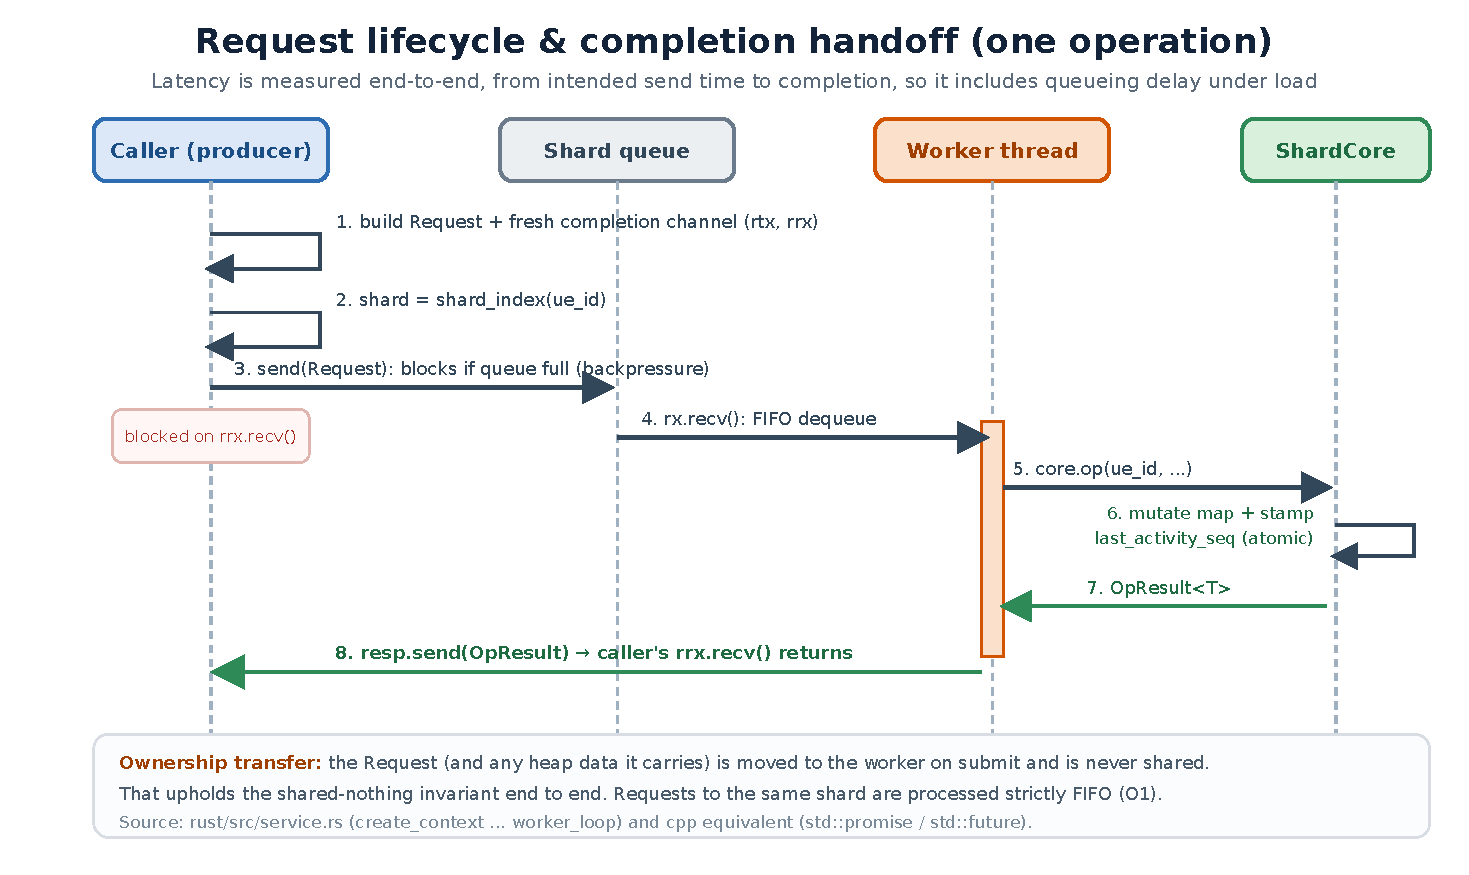
\includegraphics[width=0.78\linewidth]{diagrams/pdf/04_request_lifecycle_sequence.pdf}
\caption[The end-to-end path of a single operation]{The end-to-end path of a single operation and the completion handoff. The caller builds
a request with a single-use completion handle, routes it by \texttt{shard\_index(ue\_id)} to the
owning shard's bounded queue (blocking if it is full), and waits. The shard's single worker
dequeues in FIFO order, executes the operation against its exclusively owned store, and writes the
result back to the completion handle. Ownership of the request is transferred to the worker on
submit and never shared. Latency is measured across the whole path.\label{fig:reqlifecycle}}
\end{figure}

\begin{figure}[ht]
\centering
\begin{tikzpicture}[
    font=\small,
    prod/.style={draw, rounded corners, minimum width=2.0cm, minimum height=0.66cm, fill=blue!8},
    queue/.style={draw, minimum width=2.5cm, minimum height=0.66cm, fill=gray!12},
    worker/.style={draw, rounded corners, minimum width=2.1cm, minimum height=0.66cm, fill=red!8},
    store/.style={draw, cylinder, shape border rotate=90, aspect=0.25, minimum width=1.5cm, minimum height=0.85cm, fill=green!8},
    lane/.style={draw, dotted, rounded corners, inner sep=7pt},
    >={Stealth[length=2.4mm]}
  ]
  % producers, grouped in one box to avoid a tangle of crossing arrows
  \node[prod] (p1) at (0,1.3)  {Producer 1};
  \node[prod] (p2) at (0,0.0)  {Producer 2};
  \node[prod] (p3) at (0,-1.3) {Producer $m$};
  \begin{scope}[on background layer]
    \node[draw, dashed, rounded corners, fill=blue!3, fit=(p1)(p2)(p3), inner sep=6pt] (pg) {};
  \end{scope}
  \node[font=\scriptsize] at (0,-2.15) {load generators};

  % two representative shard lanes; spacing leaves room for the inline edge labels
  \node[queue] (q1) at (5.2,1.3)   {MPSC queue};
  \node[worker](w1) at (8.9,1.3)   {Worker 1};
  \node[store] (s1) at (12.0,1.3)  {Shard 1};
  \node[queue] (qn) at (5.2,-1.3)  {MPSC queue};
  \node[worker](wn) at (8.9,-1.3)  {Worker $N$};
  \node[store] (sn) at (12.0,-1.3) {Shard $N$};
  \begin{scope}[on background layer]
    \node[lane, fit=(q1)(s1)] (lane1) {};
    \node[lane, fit=(qn)(sn)] (lanen) {};
  \end{scope}
  \node[font=\scriptsize] at (8.35,2.35) {shard-owning threads: no shared mutable state, no locks};

  % submit: producer group -> each shard queue, routed by hash
  \node[font=\scriptsize, align=center, fill=white, inner sep=2pt] at (2.85,0) {route by\\ hash(\texttt{ue\_id})};
  \draw[->] (pg.east) -- (q1.west) node[midway, above, sloped, font=\scriptsize]{submit};
  \draw[->] (pg.east) -- (qn.west) node[midway, below, sloped, font=\scriptsize]{submit};

  % within-lane flow
  \draw[->]  (q1) -- node[above, font=\scriptsize]{FIFO} (w1);
  \draw[->]  (qn) -- node[above, font=\scriptsize]{FIFO} (wn);
  \draw[<->] (w1) -- node[above, font=\scriptsize]{owns} (s1);
  \draw[<->] (wn) -- node[above, font=\scriptsize]{owns} (sn);

  % one-shot completion: clean orthogonal return path below everything
  \draw[->, dashed, rounded corners=4pt]
      (wn.south) -- ++(0,-0.75) -- (1.4,-2.9) -- ($(pg.south east)+(-0.4,0)$);
  \node[font=\scriptsize] at (5.9,-3.05) {one-shot completion (result $\rightarrow$ waiting producer)};
\end{tikzpicture}
\caption[Shared-nothing, thread-per-shard architecture]{Shared-nothing, thread-per-shard architecture. Producers submit request messages to a
shard's bounded, blocking MPSC queue (selected by a pinned hash of the \texttt{ue\_id}) and wait
on a single-use completion handle. Each shard is read and written by exactly one worker thread,
so there are no locks on context state. Blocking on a full queue is what makes overload
observable as tail latency.\label{fig:arch}}
\end{figure}

\section{Architectural choices and technology stack}
The C++ side uses CMake with Ninja, the standard library, and \texttt{std::thread}. The Rust
side uses Cargo and the stable toolchain. Both link the same memory allocator, which keeps the
comparison about the two languages and not about two allocators: C++ links the system
\texttt{jemalloc}, and Rust installs a \texttt{jemalloc} global allocator (from
\texttt{tikv-jemallocator}). Each side also keeps a system-allocator build as a control.
Latency passes through the same high-dynamic-range (HDR) histogram
algorithm~\cite{tene_hdrhistogram} on both sides, configured the same way (range
$[1\,\text{ns}, 3.6\,\text{s}]$, three significant figures). Rust uses the standard
\texttt{hdrhistogram} crate. C++ uses a header-only port of the same bucketing algorithm,
checked against a known distribution. Build optimisation is matched as closely as the two
toolchains allow, so the Rust release profile is pinned to \texttt{opt-level~=~2} against the
C++ \texttt{-O2} build.

\section{Implementation details}\label{sec:impldetails}
\label{sec:impl}
Both implementations follow the frozen specification field for field, and both are small
enough to read end to end. The C++ core is $\CppRawLines$ lines across eight headers and two
translation units. The Rust core is $\RustRawLines$ lines across eight modules. Dropping blank
lines and comments leaves $\CppNloc$ and $\RustNloc$. Both counts describe the build the
campaign actually measures. A build flag switches on the two attribution probes of
Section~\ref{sec:idioms}, and the conditional blocks that select them are left out of the count,
because counting them would describe neither the compared build nor the probe.

The Rust version is therefore the larger of the two, by $\RawRise\%$ in raw lines and
$\NlocRise\%$ in code lines. That belongs in the text and not in a footnote, for two reasons.
Line count is one of the software-quality proxies this study set out to collect. And the
difference is not stray verbosity: it is the net of several forced idioms pulling in opposite
directions, which Section~\ref{sec:idioms} takes apart file by file.

The rest of this section works outward from the data model to the concurrency machinery. Three
of the divergences it describes carry a measured consequence, and those are the ones to read
closely. The record layout differs by $\UeCtxGapBytes$~bytes per context, the request
representation differs in both size and type safety, and the bounded queue is a primitive Rust
supplies outright where C++ has to assemble one by hand. Everything else is a matter of naming
or mechanism. Several of those cost source lines, which Table~\ref{tab:loc} accounts for, but
none changes what the two cores do.

\subsection{The UE context and the state machine}\label{sec:uecontext}
Each UE context stores its identifier, a four-value lifecycle state (\texttt{Idle},
\texttt{Connected}, \texttt{Reconfiguring}, \texttt{Released}), a fixed-size dummy security
context, and a dynamic list of data radio bearers, alongside the cell, transaction and counter
fields that Figure~\ref{fig:datamodel} sets out in full. The bearer list is deliberately a
growable container (\texttt{std::vector} / \texttt{Vec}) and not a fixed array, so that the
allocator study (RQ3) observes realistic per-context allocation. Reads return an immutable
snapshot (a \texttt{UeContextView}) copied out of the worker, not a reference into live shard
state. That keeps the shared-nothing guarantee intact and keeps the two implementations
semantically identical.

Identical field declarations do not, however, produce identical objects. Measured on the
evaluation host, a \texttt{UeContext} takes $\CppUeCtxBytes$~bytes in C++ and only
$\RustUeCtxBytes$~bytes in Rust.
Layout policy accounts for it. C++ guarantees that non-static data members sit in declaration
order, so the narrow fields the specification places between wider ones open two holes of
alignment padding. Rust carries no \texttt{\#[repr(C)]} annotation here, so it is free to
reorder fields, and it does. It packs the small scalars together and both holes close.

The specification does not try to erase that difference, and the reason is worth stating.
Pinning the Rust layout with \texttt{\#[repr(C)]} would penalise Rust for nothing but obedience
to a C++ padding rule. Hand-reordering the C++ declarations would be an optimisation the
specification asks of neither side. The gap is therefore recorded as a language-level effect and
then bounded. At the $\SweepUes$ active UEs the sweep uses, the $\UeCtxGapBytes$-byte gap comes
to roughly $\UeCtxGapTotalKB$~kB. Resident set sizes are measured in megabytes, so this does not
matter to the RQ3 comparison.

\begin{figure}[ht]
\centering
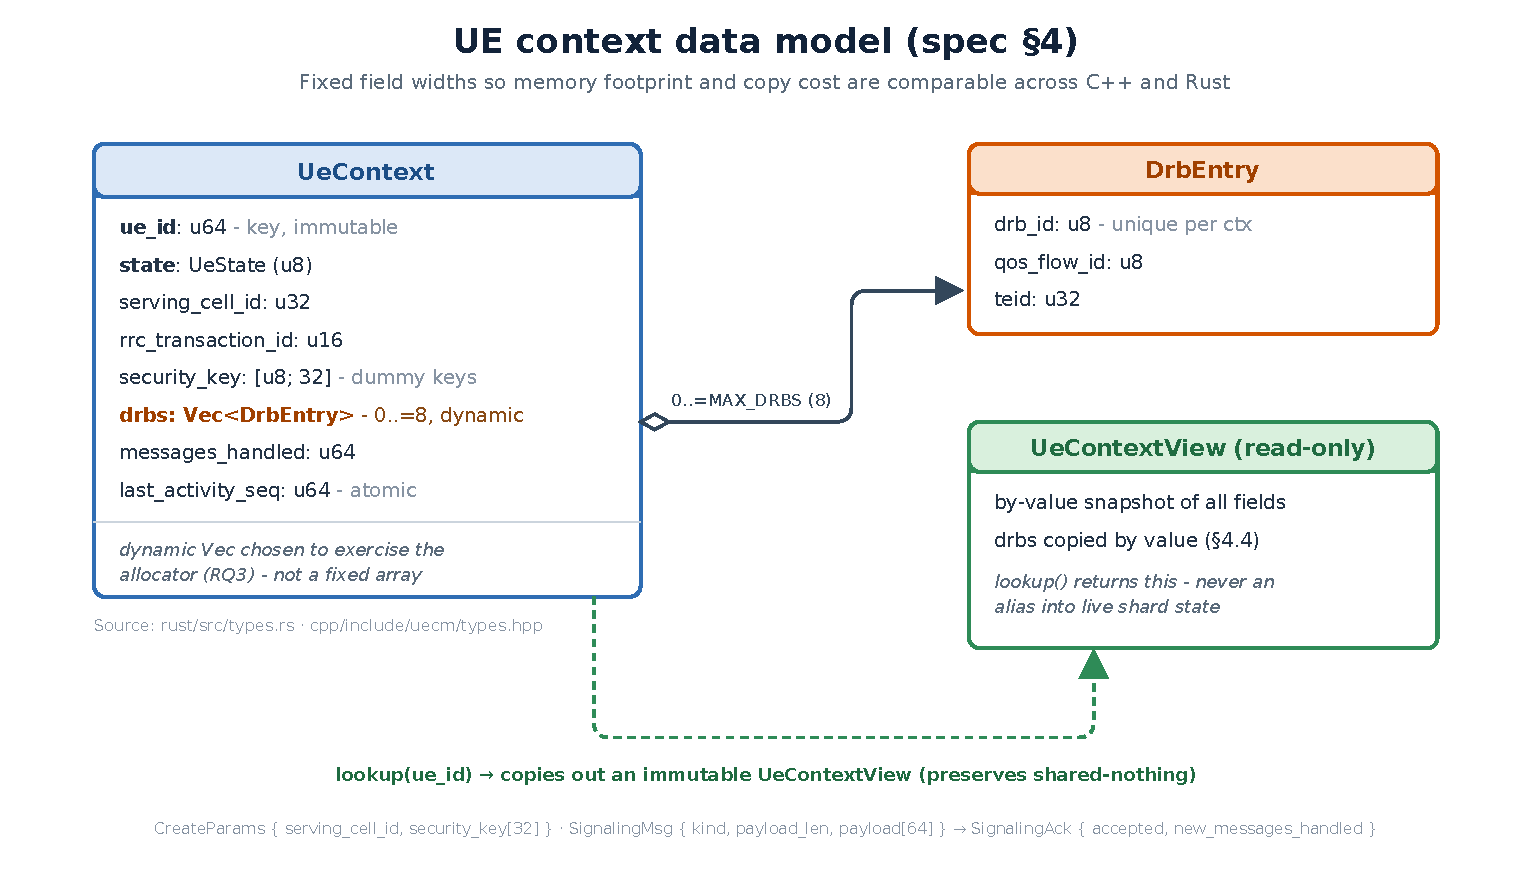
\includegraphics[width=0.72\linewidth]{diagrams/pdf/05_data_model.pdf}
\caption[The shared UE-context data model]{The UE-context data model shared by both implementations. Field widths are fixed so that
memory footprint and copy cost are comparable across languages. The data-radio-bearer list is a
dynamic \texttt{Vec}/\texttt{std::vector} on purpose, to exercise the allocator for RQ3.
\texttt{lookup} returns an immutable \texttt{UeContextView} copied out by value rather than an
alias into live shard state, preserving the shared-nothing guarantee.\label{fig:datamodel}}
\end{figure}

\subsection{Sharding, the store, and the bounded queue}
Both sides pin their hashing, so that neither standard library's hasher can become an accidental
language advantage. Shard assignment runs the \texttt{ue\_id} through the SplitMix64 finalizer,
then reduces modulo the shard count. The finalizer is three rounds of xor-shift and multiply
against constants the specification pins.
It matters because the workload draws sequential identifiers, and a naive
modulo would map those onto shards in a fixed repeating pattern. Scrambling the identifier first
makes the offered load per shard even in both languages by construction, not by luck.

The per-shard container is each language's standard hash map (\texttt{std::unordered\_map} /
\texttt{std::collections::HashMap}), but the default hashers are bypassed. They differ too much
to leave in place. C++'s \texttt{std::hash<uint64\_t>} is usually the identity function, while
Rust's default \texttt{SipHash-1-3} is cryptographically strong and correspondingly slower.
Keeping both would have measured a standard-library choice, not a language. Both maps are
therefore keyed through a pinned FNV-1a 64-bit hash over the eight little-endian bytes of the
identifier, and a test checks that the Rust \texttt{BuildHasher} produces a digest bit-identical
to the reference \texttt{fnv1a\_64}.

Both maps reserve capacity at start-up so that steady-state measurements are not disturbed by
rehashing. Every other service parameter is shared in the same way, fixed by the specification
and listed in Table~\ref{tab:params}. Only the shard count is varied from those defaults, and
only by the campaign, which sets it to match the cores it is given.

The bounded blocking queue is where the two standard libraries part company most sharply. Rust
supplies the primitive the specification asks for outright. \texttt{sync\_channel(capacity)} is
a bounded multi-producer, single-consumer channel whose \texttt{send} blocks when the queue is
full and whose \texttt{recv} blocks when it is empty, which is exactly the required
backpressure in one call. The C++ standard library, through C++23, offers no
bounded blocking queue at all. The same semantics are therefore assembled by hand from a
\texttt{mutex}, two \texttt{condition\_variable}s and a \texttt{std::queue}, in a class of
$\CppBoundedQueueLines$ lines.

The point of the comparison is not that the C++ code is badly written. It is short, it uses
the predicate form of \texttt{wait} so that spurious wakeups are handled correctly, and it
releases the lock before notifying. The point is that it exists at all. Every one of those lines
is a place where a concurrency defect could enter. And the correctness argument for it rests
with the author, not with the compiler or the library: that the two condition variables are
never confused, that the predicates match the notifications, that no wakeup is lost. This is the
same asymmetry the fault-injection study of Chapter~\ref{chapter:eval} measures, showing up here
in ordinary code with no defect in it instead of in a bug put there on purpose.

\subsection{Requests, responses, and the service lifecycle}\label{sec:tagged}
\label{sec:request}
The message type carried through that queue is the second forced divergence. Rust models a
request as an \texttt{enum} with one variant per
operation. Each variant carries exactly its own arguments plus a \texttt{Sender} parameterised
by exactly that operation's result type. C++ has no payload-carrying
enumeration in the standard idiom used here, so a request is a tagged struct instead. It holds an
\texttt{OpKind} discriminant alongside \emph{every} argument field any operation might need,
paired with a single \texttt{std::promise}. That promise's value type must therefore be a
\texttt{std::variant} over all four possible result types.

This has three measurable consequences. The first is size. A \texttt{Request} is $\CppRequestBytes$~bytes
in C++ against $\RustRequestBytes$ in Rust, because the C++ struct always carries the create parameters, the
$\SignalingMsgBytes$-byte signalling message, the bearer entry, and the reconfiguration parameters, whether
the operation in flight uses them or not. The Rust enum is sized by its largest variant
alone. With the default eight shards holding up to $1\,024$ requests each, full occupancy means roughly $\CppQueueResidentMB$~MB of
queue-resident request storage against $\RustQueueResidentMB$~MB. The second consequence is a copy cost
paid on every submission, because the unused fields are default-initialised and moved along with
the used ones.

The third matters most to the argument of this thesis, and it is a type-safety
gap. The C++ caller has to recover its typed result from the variant with
\texttt{std::get<OpResult<T>>}, which throws \texttt{std::bad\_variant\_access} if the worker
ever writes an alternative the caller did not expect. That exception cannot fire in the
code as it stands, because each \texttt{OpKind} is handled by exactly one branch and that branch
stores the matching alternative. But the invariant behind it is upheld by reading two
files, not by the compiler. Rust settles the same invariant by construction. The sender embedded
in each variant is already typed, so there is no response union, nothing to unwrap, and no
runtime dispatch on the way back.

Starting the service allocates the shards, spawns one worker thread per shard, and hands each
worker exclusive ownership of its store. The request path is then the one described in
Section~\ref{sec:concurrency}. Shutdown is the more delicate half, because it has to stop
workers blocked on an empty queue without abandoning requests still in flight. Both
implementations solve it the same way. An in-band \texttt{Stop} sentinel is pushed onto each
shard's queue, and strict FIFO order means every request ahead of it completes first, so no
closed flag or drain API is needed and no completion handle is left unfulfilled. The worker
threads are then joined. Both languages tie all of this to object destruction, which is one of
the few places the two are near-identical, and both make it idempotent, so a service that goes
out of scope can neither leave detached threads behind nor stop twice.

The window between \texttt{start()} and \texttt{shutdown()} is a precondition on every
operation, and it is written as one. An operation submitted outside that window is a caller
error and not a runtime condition, so it is reported out of band and does not widen the closed
\texttt{OpError} set of Section~\ref{sec:parity}. C++ throws \texttt{std::logic\_error} and Rust
panics. Saying so explicitly was not a formality. The specification forbade the call from the
start, neither implementation checked it, and in that gap the two languages did not fail alike.
The episode is reported with the safety results in Section~\ref{sec:safetyresults}, because a
defect found in code written to be correct carries evidence an injected one cannot.

One more piece of ownership discipline holds the shared-nothing invariant together end to end. A
request is moved into the queue and not copied, and it carries its completion handle with it, so
the producer and the worker never both hold a usable reference to the same request. C++ enforces
this by making \texttt{Request} move-only, a property it picks up automatically from the
move-only \texttt{std::promise} it contains. In Rust it follows from ordinary move semantics, and
the compiler rejects any attempt to use the request after submission. The only shared mutable
state in either implementation is the atomic activity counter. C++ holds it by reference, Rust as
a cloned \texttt{Arc<AtomicU64>}, and both increment it with relaxed ordering because nothing
branches on its value.

\subsection{Forced idioms, and what the two cores cost}
\label{sec:idioms}
Where the two languages must diverge to satisfy the same requirement, the deviation is
recorded in the specification's forced-idiom log so that it can be weighed rather than
silently absorbed into the results. Table~\ref{tab:idioms} collects the log in full, and the
preceding subsections have already quantified the two entries with measurable consequences.

\begin{table}[H]
\centering
\small
\caption[The forced-idiom log]{The forced-idiom log: every point at which the two implementations diverge in order
to satisfy the same specification requirement, with the measured consequence where there is
one.\label{tab:idioms}}
\begin{tabular}{@{}R{0.20\linewidth} R{0.36\linewidth} R{0.36\linewidth}@{}}
\hline\hline
Concern & C++ & Rust \\
\hline
Result type & \texttt{std::expected<T, OpError>} & \texttt{Result<T, OpError>} \\
Request & tagged struct: discriminant plus every argument field ($\CppRequestBytes$\,B) & \texttt{enum}, one variant per operation, carrying only its own arguments ($\RustRequestBytes$\,B) \\
Response & \texttt{std::variant} of four result types, unwrapped by the caller with \texttt{std::get} & none needed: each variant carries a sender of its own result type \\
Bounded queue & hand-written \texttt{mutex} plus two \texttt{condition\_variable}s ($\CppBoundedQueueLines$ lines) & \texttt{sync\_channel(capacity)} \\
Completion & \texttt{std::promise} / \texttt{std::future} & a fresh \texttt{mpsc::channel()} per request \\
Per-shard map & \texttt{std::unordered\_map} with an \texttt{FnvHash} functor & \texttt{HashMap} with an \texttt{FnvBuildHasher} \\
Activity counter & \texttt{std::atomic<uint64\_t>} held by reference & \texttt{Arc<AtomicU64>} cloned into each worker \\
Teardown & destructor calls \texttt{shutdown()} & \texttt{Drop} calls \texttt{shutdown()} \\
Optimisation level & \texttt{-O2} & \texttt{opt-level = 2} \\
\hline
\end{tabular}
\end{table}

The log also explains the line-count difference reported at the head of this section, and it
says more than the net figure does, because the contributions do not all point
the same way. Table~\ref{tab:loc} breaks the $\LocGap$-line gap down by concern. Rust is
much \emph{shorter} in exactly one place, the bounded queue, where it needs no code
at all against $\CppBoundedQueueLines$ lines of C++. It is longer almost everywhere else, and
three entries account for most of that excess.

The largest is the service module, for the reason given above. Because the C++ response is a
single \texttt{variant}, all ten public operations funnel through one shared \texttt{submit}
helper, and each typed wrapper shrinks to two or three lines. Rust's per-variant typed
sender admits no such helper without generics, so every operation repeats the same sequence:
create a completion channel, construct its variant, send, receive. The next entry shows the
trade-off most clearly, and it is hashing. C++ meets
\texttt{std::unordered\_map}'s hasher requirement with a five-line functor wrapping
\texttt{fnv1a\_64}. Rust has to supply the whole trait apparatus, every line of it
boilerplate, and what it buys is a statically dispatched, type-checked hasher instead of a
callable of the conventional shape. The third entry is the module tree and public re-export
list, work C++ gets for free from its header structure.

None of this is a defect on either side, and none of it shows up in the performance figures.
It is the kind of engineering cost the forced-idiom log exists to expose. Rust spends source
lines on trait machinery and repetition at the call site, and what it gets back are guarantees
the compiler can check. It then wins much of that spend back wherever its standard library
happens to supply a primitive that C++'s does not.

Counting lines, however, answers only half the question a reviewer of either codebase would
ask, because it treats a line of boilerplate and a line of branching as the same thing.
Table~\ref{tab:complexity} therefore adds cyclomatic complexity, measured by
\texttt{lizard}~\cite{lizard} over both cores. One tool applied to both languages is what makes
the figures comparable, because it uses the same definition of a decision point on each side.
Each language's own tooling would count somewhat different things. The two measures then
point in opposite directions. Rust is $\NlocRise\%$ longer than C++ by code lines, but its
total cyclomatic complexity is $\CcnTotalDrop\%$ \emph{lower}, $\RustCcnTotal$ against
$\CppCcnTotal$, spread over slightly more functions ($\RustFuncs$ against $\CppFuncs$). Both
cores are undemanding by the usual thresholds, and both have a median per-function complexity
of one, so a small number of functions at the top carry the aggregate.

That top is where the difference sits, and it traces back to a divergence already described,
not to anything spread thin. The most complex function in the C++ core is
$\CppCcnMaxFn$ at $\CppCcnMax$, more than twice its Rust counterpart's $\RustCcnMax$. It
switches on the \texttt{OpKind} discriminant and then stores the matching alternative into the
response \texttt{variant}. The tagged-struct design of Section~\ref{sec:tagged} therefore
gathers the whole dispatch, and the correctness argument that goes with it, into one branch-heavy
function. Rust's per-variant typed sender removes the return-path dispatch altogether, which is
why its worker has nothing comparable to unwrap. The trade is sharper than the line
count alone suggested. The extra lines Rust spends buy back branching in the one place where
branching is hardest to review. And the \texttt{std::bad\_variant\_access} invariant that
Section~\ref{sec:tagged} described as upheld by reading two files lives inside
exactly the function this measurement flags.

\begin{table}[H]
\centering
\small
\caption[Size and cyclomatic-complexity proxies for the two cores]{Size and cyclomatic-complexity proxies for the two cores, measured with
\texttt{lizard}~\cite{lizard} applied identically to both languages. Benchmark drivers, tests,
conformance runners, the FFI seam, and the probe-conditional blocks of
Section~\ref{sec:idioms} are excluded. Only the compared code the parity contract constrains is
counted. Complexity is one plus the number of decision points in a function. The line count is
NLOC as \texttt{lizard} defines it, which also discounts brace-only and preprocessor lines. It
is the same measurement quoted at the head of
Section~\ref{sec:impldetails}.\label{tab:complexity}}
\begin{tabular}{@{}l r r@{}}
\hline\hline
Measure & C++ & Rust \\
\hline
Files & 10 & 8 \\
Functions & 37 & 42 \\
Lines of code (blank and comment lines excluded) & 517 & 621 \\
Total branching complexity & 95 & 83 \\
Mean complexity per function & 2.6 & 2.0 \\
Median complexity per function & 1 & 1 \\
Most complex function & 13 (\texttt{worker\_loop}) & 6 (\texttt{add\_drb})
\\
\hline
\end{tabular}
\end{table}

\begin{table}[H]
\centering
\small
\caption[Where the line-count difference between the cores comes from]{Where the $\LocGap$-line difference between the two cores comes from, by concern (raw
lines, including comments. C++ figures merge header and translation unit. Probe-conditional
blocks excluded as in Section~\ref{sec:impldetails}). Rust is shorter
only where its standard library supplies a primitive C++ lacks.\label{tab:loc}}
\begin{tabular}{@{}R{0.38\linewidth} r r r@{}}
\hline\hline
Concern & C++ & Rust & $\Delta$ \\
\hline
Service (queues, workers, API) & $234$ & $291$ & $+57$ \\
Hashing (functor vs.\ trait pair) & $37$ & $70$ & $+33$ \\
Module tree and re-exports & $0$ & $26$ & $+26$ \\
Message types & $48$ & $67$ & $+19$ \\
Data model & $73$ & $85$ & $+12$ \\
Configuration & $18$ & $29$ & $+11$ \\
Shard core (state machine) & $182$ & $188$ & $+6$ \\
Error model & $32$ & $26$ & $-6$ \\
Bounded queue & $51$ & $0$ & $-51$
\\
\hline
Total                             & $\CppRawLines$ & $\RustRawLines$ & $+\LocGap$ \\
\hline
\end{tabular}
\end{table}

One property of the Rust core is not a cost at all, and it closes this section because it is what
the costs above bought. The Rust library contains \emph{no} \texttt{unsafe} code, and that is
checked mechanically over the crate. Safe Rust therefore guarantees data-race freedom for this core at
compile time, through the \texttt{Send} and \texttt{Sync} traits. The shard store is owned by a
single worker and never shared, the request type is moved across the thread boundary, and the
one piece of genuinely shared state, the activity counter, is an atomic. None of this needs a
runtime sanitiser to establish, and none of it needs test coverage to hold. The C++
implementation does no manual memory management beyond STL containers and no explicit
locking outside the queue class, and it was checked data-race free under ThreadSanitizer.

The two statements are not, however, evidence of the same kind, and that difference is the
thesis's central safety claim in miniature. The Rust property is a theorem about the program,
discharged by the compiler on every ordinary build and covering every execution. The C++
property is an observation about the executions a particular instrumented binary happened to
take, and it would have to be re-established after any change, on a build most projects do not
run by default. Quantifying exactly how far apart those two kinds of assurance are is the
purpose of the fault-injection study in Chapter~\ref{chapter:eval}.

\section{Public API and operation semantics}
Both implementations expose the same small, lifecycle-oriented API against the shared
specification, so the surface a caller sees is identical apart from each language's naming
conventions. A service is created with a fixed shard count and a per-shard queue bound.
Callers then invoke context operations, each identified by the target \texttt{ue\_id}: create,
setup, handle-signalling, add-bearer, reconfigure begin/complete/abort, release, and state
lookup. Every operation is \emph{total} and \emph{typed}. It returns either a success value or
a typed \texttt{OpError} drawn from a closed five-value enumeration (\texttt{NotFound},
\texttt{AlreadyExists}, \texttt{InvalidState}, \texttt{CapacityExceeded} and
\texttt{InvalidArgument}). An operation that is illegal for the context's
current state (Figure~\ref{fig:fsm}) returns the matching error and leaves the context
untouched. It does not mutate the context, and it does not signal failure out of band.

That choice matters for fairness as much as for correctness. Neither implementation uses
exceptions or error codes as a hidden control-flow channel, so the cost and the control flow of
the failure path are visible and identical on both sides. It also means the same conformance
vectors (Section~\ref{sec:parity}) can assert op-for-op agreement on both the returned value and
the resulting state.

Two points in that semantics need stating, because the state machine as drawn hides them.
\texttt{Released} is never stored: \texttt{release\_context} erases the entry, so the state is a
passing label rather than one an implementation can rest in, and a second release returns
\texttt{NotFound} and not \texttt{InvalidState}. And \texttt{abort\_reconfigure} restores the
\emph{state} to \texttt{Connected} without restoring the serving cell
\texttt{begin\_reconfigure} overwrote, because the model keeps none to roll back to. That is a
deliberate simplification and a semantic commitment either way, and the parity suite of
Section~\ref{sec:parity} holds both languages to it.

\section{Parity verification}
\label{sec:parity}
The whole comparison rests on the two versions being functionally identical, so parity
is tested and not assumed. A language-neutral conformance suite writes test vectors as
sequences of operations with their expected results and an expected post-state summary. A
runner in each language executes the vectors and emits a transcript in one fixed format, and the
two transcripts are diffed for op-for-op agreement. The seeded suite covers the full error model,
the reconfiguration begin/complete/abort paths, data-radio-bearer fill and overflow, and
shard-assignment determinism. Both implementations currently pass and agree. The benchmark
workloads add a second parity signal, independent of the first. For a given seed and active-UE
population, the mixed workload's per-operation-kind counts are checked to be identical across
languages, which confirms that both implementations are driven along exactly the same code paths.

Two things bound what that establishes, and both are answered rather than conceded. A
cross-diff of two implementations cannot tell ``both correct'' apart from ``both wrong in the
same way'', and that is the failure mode a shared specification and a single author make most
likely. The expected results in the hand-written vectors also came from the
specification by way of the person who wrote the implementations. A third implementation of the
same written specification therefore acts as an independent oracle. It is written in Python,
shares no code with either language, and has to reproduce all $\ConfHandOps$ hand-derived
expectations before it is allowed to generate any of its own. It then generates randomised
operation sequences under several profiles: realistic lifecycles, adversarial sequences
weighted towards illegal transitions, sequences that sit on the capacity limits, and sequences
that stress shard assignment. The model computes every expected result. A campaign
of roughly $\ConfGenOps$ generated operations produced no divergence at all. The two
implementations agree with each other, and with an independent reading of the specification, on
sequences nobody chose. The generator is seeded and deterministic, so any future divergence is a
permanently reproducible regression and not an anecdote.

Three further checks bound the suite from other directions. The specification's transition
matrix is walked exhaustively and not sampled: every operation applied to a context in
every state it can occupy. Each case asserts the exact error, the resulting state on success, and
the absence of any field change on failure, including the error precedences the specification
leaves unordered. The C++ implementation is then run under AddressSanitizer, ThreadSanitizer
and UndefinedBehaviorSanitizer across that whole suite, and reports nothing. That matters for
fairness. Safe Rust carries data-race and memory-safety freedom by construction, so without
the sanitiser run the C++ arm's equivalent property would rest on not having failed yet instead
of on having been checked. Miri, run over the Rust state-machine suite, likewise reports no
undefined behaviour. Third, the suite's reach is measured and not asserted, because a
negative result from a sanitiser is only as broad as the code that ran. Line coverage of the
C++ library is $\CppLineCov\%$ and of the Rust library $\RustLineCov\%$, and both implementations' core
operation processors and service facades are fully covered. The two figures are not strictly
comparable, because \texttt{gcov} and \texttt{llvm-cov} do not resolve an executable line alike.
On the finer-grained regions \texttt{llvm-cov} counts, the Rust figure is $\RustRegionCov\%$.
Each bounds the claims made about its own implementation.

\chapter{Experimental Setup and Evaluation\label{chapter:eval}}

\section{Testbed configuration\label{sec:testbed}}
This chapter reports two kinds of result. Some follow from the compilers and the source. Others
depend on the machine. Both kinds are now measured on a host that meets the protocol of
\texttt{bench/TESTBED.md}, which was not true of the campaign this study ran for most of its
life. Table~\ref{tab:testbed} describes the machines and keeps the split clear.

\paragraph{The environment used.}
Every performance number in this chapter comes from one dedicated bare-metal server: a
single-socket \MainCpu{} with \MainCores{} cores on \MainNumaNodes{} NUMA node, simultaneous
multithreading \MainSmt{}, kernel \MainKernel{}. The frequency governor is fixed at
\MainGovernor{} with boost disabled, so the cores hold their base clock rather than a thermally
negotiated one, and cores \MainPinned{} carry the benchmark. The environment capture records
virtualisation as \MainVirt{}. Every run records the environment metadata of
Section~\ref{sec:repro}.

The toolchain is not the host's. Both implementations are built and run inside a pinned container
image carrying \MainDistro{} with \texttt{g++~\MainGpp} and \texttt{rustc~\MainRustc}, which is the
same userspace and compiler pair the earlier virtualised campaign used. Fixing the toolchain in an
image is what allows a change of machine to be a change of machine only: the container shares the
host's kernel, scheduler and clocksource, so it buys toolchain identity and nothing else, and it is
the reason the two campaigns compared in Section~\ref{sec:hostcompare} differ in the hardware
alone.

Two properties of this host are worth stating before any tail number is read, because they are what
the previous host lacked. There is no hypervisor between the benchmark and the cores, so no
timeslice is lost to a machine this study cannot observe. And the kernel runs tickless on the
pinned cores (\texttt{nohz\_full}), which removes the periodic timer interrupt from the measured
path. What the host does \emph{not} have is \texttt{isolcpus}, and that omission is deliberate
rather than an oversight: isolating the cores also removes them from every scheduling domain, and
because the benchmark pins its threads to a range and relies on the kernel to spread them, an
isolated set collapses all of them onto one core. Section~\ref{sec:threats} records the cost.

\paragraph{The host this study measured on first, and why it appears at all.}
Until late in the work the campaign ran on a virtualised host: a \GuestCpu{} guest,
\GuestCores{} vCPUs, \GuestVirt{} virtualisation, no core isolation. Three of this chapter's
results were already settled there, and one was not settleable there at all. The obstacle was not
a shortage of repeats. On that host the $95\%$ confidence interval on a single variant's p99 spans
$\GuestPNineNineMaxCI\,\mu$s while the four variants' p99 values differ by
$\GuestPNineNineRange\,\mu$s, so the uncertainty about one swamped the gap between all of them.

That campaign is not discarded, and Section~\ref{sec:hostcompare} reports it against the present
one. The two share a design exactly, the same \GuestShards{} shards and \GuestProducers{}
producers over \GuestLoadLevels{} load levels at \GuestRepeats{} repeats, so what separates them is
the machine. A comparison of that kind is the only direct evidence this study can offer that its
instrument is now adequate to the questions it asks, and one of its findings is that a quantity
this thesis once reported as a language-independent property of allocators was in part a property
of that machine.

\paragraph{Measurement discipline common to both.}
On any host, Section~\ref{sec:stats} applies: each sweep point is a median over \NRepeats{}
interleaved repeats with a bootstrap $95\%$ confidence interval. Interleaving shares interference
across variants. Absolute latency suffers, but comparative C++/Rust conclusions remain valid.
Throughput is counted over the measured phase only, warm-up excluded.

Table~\ref{tab:testbed} does not rank results by importance. It separates what compilers and
source settle from what only the machine can settle.

\section{Workload and evaluation measurements\label{sec:workload}}
A synthetic but spec-justified telecom workload is generated by a deterministic driver whose
structure both implementations share, so the two versions are exercised along identical
code paths. Two workloads are provided. The \emph{signal} workload preloads a population of
connected UEs and then hammers the \texttt{handle\_signalling} hot path, which isolates
steady-state per-message latency. The \emph{mixed} workload is a pinned RAN lifecycle generator.
It walks each UE through a realistic procedure sequence, context creation, connection setup,
signalling, bearer setup, reconfiguration/handover (begin/complete/abort), and release, using a
fixed SplitMix64 draw order and a per-slot expected-state model so that every operation it emits
is valid. The fixed draw order means the per-operation-kind counts are identical in C++ and
Rust for a given active-UE population and seed, which doubles as the parity signal described in
Section~\ref{sec:parity}. The control parameters are the target event rate and the number of
active UEs, swept from nominal load through saturation and overload. The send schedule is fixed
and the histogram is corrected, so a stall introduces no coordinated-omission
bias~\cite{schroeder2006openclosed,tene_hdrhistogram}. Three measurement campaigns are run: a load sweep for
performance, the fault-injection study, and an FFI migration prototype.
Figure~\ref{fig:workload} shows the two workloads and the procedure sequence the mixed one
walks.

\begin{figure}[ht]
\centering
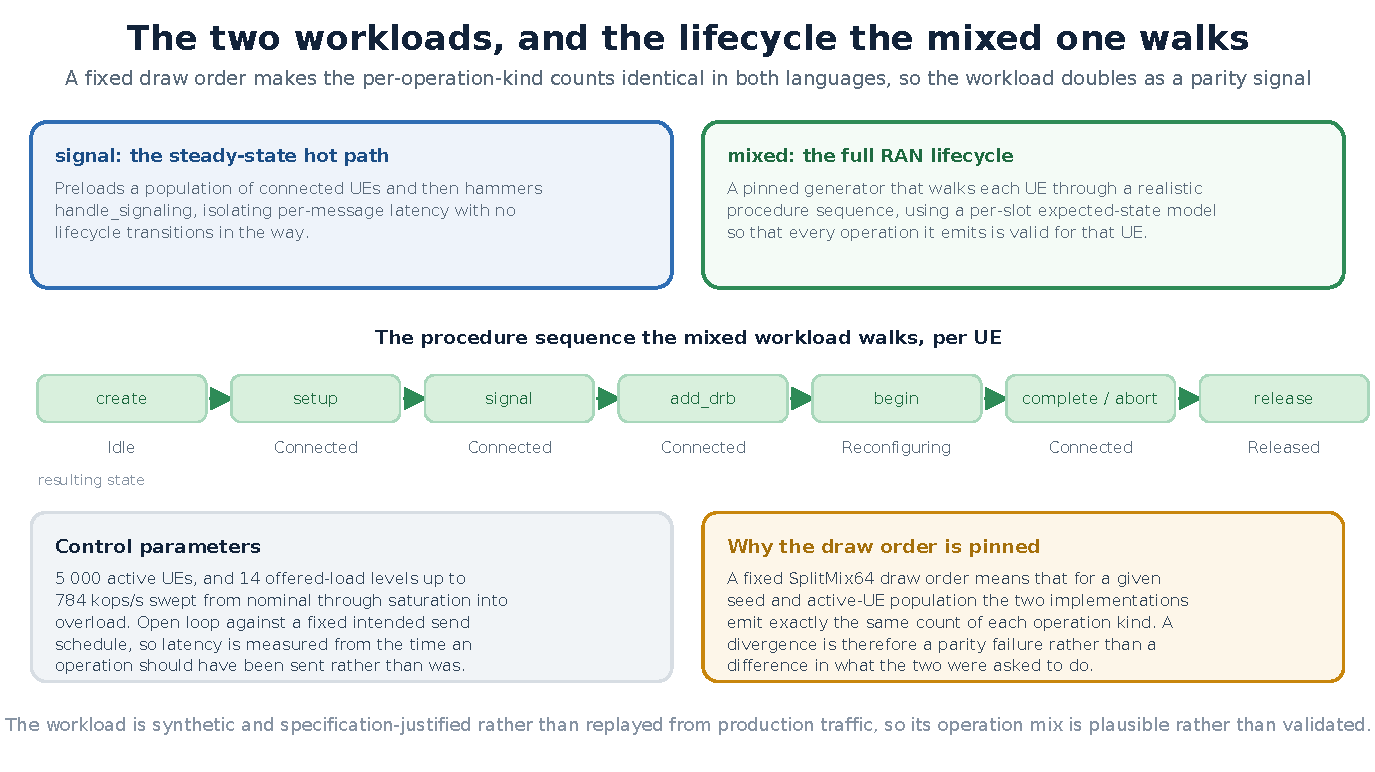
\includegraphics[width=0.78\linewidth]{diagrams/pdf/27_workload_timeline.pdf}
\caption[The two workloads, and the lifecycle the mixed one walks]{The two workloads. The \emph{signal} workload isolates the steady-state hot path.
The \emph{mixed} workload walks each UE through the full RAN procedure sequence, with a
per-slot expected-state model ensuring that every operation it emits is legal for the state
its context is actually in. Because the SplitMix64 draw order is pinned, a given seed and
active-UE population produce identical per-operation-kind counts in both languages, so a
divergence is a parity failure rather than a difference in what the two implementations were
asked to do.\label{fig:workload}}
\end{figure}

\paragraph{What ``spec-justified'' claims, and what it does not.}
The term is used precisely, because the distinction bounds what the workload can support. The
\emph{sequence} of operations is justified. It is the RRC connection lifecycle the 3GPP
specifications define for a UE, from establishment through in-session signalling and bearer setup
to reconfiguration and release~\cite{3gpp38401,3gpp38331}. The per-slot expected-state model then
guarantees that every operation the driver emits is legal for the state its context is actually
in, so the workload never drives the service down a path the specification forbids. The
\emph{proportions} are not justified in the same way. How often a real cell hands over, against
how often it establishes a bearer, depends on deployment, mobility, and time of day, and no
public figure fixes it. The mix used here is therefore plausible and not validated.
Section~\ref{sec:threats} reports that as a threat to external validity, and trace replay heads
the future-work list for exactly this reason.

For a \emph{comparative} question the distinction costs less than it would for an absolute one,
and saying why is part of arguing that the data suits the task. Both implementations execute the
same sequence in the same order for a given seed and active-UE population, and the
per-operation-kind counts verify it. An unrepresentative mix therefore shifts both languages
equally and cannot manufacture a difference between them. An unvalidated operation mix bounds how
far the numbers travel. It does not compromise the fairness of the comparison they are used to make.

Table~\ref{tab:params} gathers the configuration of the service, the workload and the campaign in
one place. Those values are otherwise spread across the specification,
Chapter~\ref{chapter:design}, and this chapter. That is convenient while reading each in turn, and
unhelpful to anyone trying to reproduce the campaign or to judge whether a parameter was chosen to
suit the result. Every entry in the campaign block is either fixed by the specification or
generated from the measurement logs, so none of it can drift out of step with the data reported
below. Two operating points are used throughout what follows, and the first of them is fixed
rather than derived. The representative point sits at $\ReprLoad$~kops/s, against a measured
throughput plateau of $\SatKnee$~kops/s, and saying why it is fixed is worth a short paragraph
because the alternative was tried and failed.

The rule this study began with took the busiest swept load at which all four variants still held
their p99 below $5$~ms. That rule is retained as a diagnostic and is no longer the operating point,
because it turns out to measure the machine rather than the service. On the virtualised host it
returned $\GuestDeadlineLoad$~kops/s, where p99 sat just under the deadline, so it was locating where
that host's interference reached $5$~ms. On a quiet host p99 stays near
$\PNineNineTrackingTop\,\mu$s until capacity binds, so the same rule climbs to the tracking limit and
collapses the representative point onto the saturation knee. One rule, two different quantities,
decided by how noisy the machine was. Fixing the point instead costs the appearance of derivation and
buys two things that matter more: the two hosts are compared at the same offered load, and the point
stays below saturation on both, which every below-saturation claim in this chapter already assumes.

\section{Evaluation data}
Four campaigns produce four datasets, and they differ in kind and not only in content. What
follows describes each one as captured, because judging whether the analysis is sound takes
knowing what was recorded and at what level of detail. Every measured
quantity this chapter quotes reaches the page as a generated macro. That script
(Section~\ref{sec:repro}) rebuilds all of them, along with every figure and table body, from the
raw logs, so a rerun moves the prose and cannot leave a headline number behind. The
software-quality
proxies are not gathered here but reported where they read most clearly: beside the
forced-idiom log they explain (Table~\ref{tab:complexity}), and beside the FFI seam, the only
place either implementation contains \texttt{unsafe} (Table~\ref{tab:ffi}).

\paragraph{The performance sweep.}
Each of the $\NRuns$ runs of the factorial design in Table~\ref{tab:params} contributes one
record, written as newline-delimited JSON. A campaign is therefore an append-only log and not a
summary table. Nothing is aggregated at capture time, and every statistic in this chapter is
recomputed from the raw records. A record carries the run's configuration (language, allocator,
workload, shard and producer counts, target rate), its outcome (operations completed, errors,
wall-clock duration, achieved throughput), the latency distribution read out of the HDR
histogram (mean, p50, p90, p99, p99.9, maximum, in nanoseconds), the resource counters taken
through \texttt{getrusage} (peak resident set size, user and system CPU seconds, CPU
utilisation), and the per-operation-kind counts. Keeping the kind counts in every record is
what makes a divergence between the two languages show up as a parity failure
(Section~\ref{sec:parity}) instead of being mistaken for a performance difference.

\paragraph{The component decomposition and contended primitives.}
The second measurement level of Section~\ref{sec:methodperf} yields a much smaller dataset of a
different shape. For each of \BudgetRepeats{} interleaved repeats it records the batch-mean cost
in both languages, once for the operation called directly and once for the same operation called
through the threaded
service. A third dataset, of the same paired shape over \ContentionRepeats{} repeats, records
sustained throughput through the bounded queue and completion primitives alone
(Section~\ref{sec:contention}). The FFI comparison of Section~\ref{sec:migrationresults} has the
same structure over \FfiOpRepeats{} repeats. All three are paired by construction, which is what
the exact paired test of Section~\ref{sec:stats} requires.

\paragraph{The fault-injection catalogue.}
This dataset is categorical and not numeric. Each of the $\FaultClasses$ defect cases yields four
tool
logs: the AddressSanitizer, ThreadSanitizer and UndefinedBehaviorSanitizer output for the C++
program, and the \texttt{rustc} output for the safe-Rust counterpart. Each case also yields one
row in a machine-readable taxonomy, recording the three sanitiser outcomes, the detection stage,
the compiler result with the diagnostic codes that fired, and the expectation registered before
the study. The two original boundary cases yield a second table from the model checkers, and the
\texttt{unsafe} one a third from the interpreter. Carrying
the expectation in the data instead of in the prose is what lets the runner report a mismatch
in either direction. The table and figure in Section~\ref{sec:safetyresults} are generated from
those logs (Section~\ref{sec:repro}), not transcribed from them.

\paragraph{What travels with the data.}
Every campaign writes the environment record of Section~\ref{sec:repro} beside its results,
\emph{including} the fields a given host does not expose. That last detail matters more than it
sounds. The governor and turbo state are stored as unavailable rather than left out, so the
limitation documented in Section~\ref{sec:testbed} is a property of the dataset itself and not
only of the prose describing it, and a reader can check it without taking it on trust.

\paragraph{The second bare-metal campaign.}
A further dataset carries the sweep's record and adds to it in three ways, two of them things the
virtualised host could not produce at all. Its latency block is wider, with the quartiles, the standard
deviation and p99.99 beside the percentiles listed above. Each run also persists its complete HDR
bucket contents to a sidecar, so the repeats can be pooled into one distribution before a far-tail
percentile is read off, and a separate file records \texttt{perf} counters at two scopes, the
end-to-end path and the operation on its own. Last, every run on a \texttt{jemalloc} arm records
that allocator's own accounting of the process, which is what lets
Section~\ref{sec:baremetal} decompose the resident set instead of bounding it by elimination. The
system-allocator arms store those fields as unavailable rather than as zero, on the same principle as
the governor and turbo state. The same scripts read all of it, so nothing
in the analysis changes between the two hosts. What does change is the answer, which is why the two
are reported apart rather than merged: this dataset confirms the sweep's findings on a quiet machine
and does not replace its numbers, for the design reasons Section~\ref{sec:baremetal} closes with.

\section{Evaluation results}
The safety results do not depend on the measurement host at all, and the migration results depend
on it along one axis only. The performance and resource results do, and
Section~\ref{sec:testbed} states what that host can and cannot carry. Every figure and table
below is measured on it unless stated otherwise.

Resolved and unresolved outcomes are reported side by side, because saying at the outset which is
which keeps a null result from being read as an absent one. Every comparison below resolves on this
host, including the far tail \emph{below} saturation, which was the one open question of this study
for as long as it measured on a virtualised machine.
Section~\ref{sec:hostcompare} sets that change beside the earlier host, because the difference
between the two is a result about measurement rather than about either language, and it is reported
last among the performance results for that reason. One resolved outcome is resolved only as a
measurement and not as a mechanism, the divergence past saturation, and
Section~\ref{sec:contention} reports how far the mechanism could be narrowed.

\subsection{Below saturation (RQ1, RQ3)}\label{sec:perfresults}
The hypothesis under test is H1 (Section~\ref{sec:rqs}): equivalence below saturation, with any
difference confined to the far tail. The absolute figures belong to the host of
Section~\ref{sec:testbed}, each point aggregates \NRepeats{} interleaved repeats, and reported
values and shaded bands are medians with nonparametric bootstrap $95\%$ confidence intervals.

Table~\ref{tab:latency} summarises the per-operation latency distribution at the representative
load of Section~\ref{sec:workload}, $\ReprLoad$~kops/s, a point at which all four build
variants are simultaneously healthy and so a fair place to compare them.

The four variants sit within $\PFiftyRange\,\mu$s of one another at the median, or
$\PFiftySpread\%$, which is the magnitude a deployment would care about and it is negligible. The
\emph{ordering} is nonetheless legible: the two Rust intervals sit below the two C++ intervals with
no overlap between the languages, while the two allocators of one language overlap each other. So
the table already suggests what the paired test below confirms, and the two instruments agree here
in a way they did not on the previous host, where every interval at this percentile overlapped every
other.

That agreement extends up the distribution, and stating why takes one comparison. The p99
values differ by $\PNineNineRange\,\mu$s across variants while the widest $95\%$ confidence
interval on a single variant's own p99 spans $\PNineNineMaxCI\,\mu$s, so the uncertainty about one
variant is smaller than the gap between them. That relation is what licenses an ordering, and it is
the relation this study could not obtain for most of its life: on the virtualised host the same two
quantities were $\GuestPNineNineRange\,\mu$s and $\GuestPNineNineMaxCI\,\mu$s, the wrong way round
by a factor of five. Section~\ref{sec:hostcompare} sets the two hosts side by side, because the
difference between them is a result about measurement rather than about either language.

The tail rows of Table~\ref{tab:significance} therefore carry a finding rather than a shrug, and
the instrument that carries it is the corrected $p$-value and not the interval. Both p99 rows and
both p99.9 rows clear the Holm correction, \NTailExclZero{} rows in all, with the same direction as
at the median. Their intervals also exclude zero, and Section~\ref{sec:stats} fixes in advance that
an interval in this block is not read as a finding, so the intervals are reported and left to one
side. That rule was written against a host whose hypervisor disturbed exactly these percentiles. It
is kept here rather than relaxed, because a rule that is dropped once the machine improves was never
a rule, and keeping it costs nothing: the correction resolves these rows on its own.

Predictability is evidenced as far as p99.99, and that column is a different statistic from the rest
of its table. It is one percentile of the four variants' repeats concatenated, between
\FarTailSamplesMin{} and \FarTailSamplesMax{} operations per variant, which is what
Section~\ref{sec:stats} means by pooling: a single run holds on the order of seventeen observations
past p99.99, too few for the percentile to mean anything, and the campaign persists every run's full
histogram buckets so the repeats can be combined after the fact. Pooling takes the operation as the
unit of analysis, so the column has no across-repeat interval to print and none is printed. Read that
way the far tail separates the languages outright: the widest gap between variants is
$\FarTailRange\,\mu$s, $\FarTailSpread\%$ of the smallest, and both \FarTailLower{} variants sit
below both of the others.

\begin{table}[H]
\centering
\small
\caption[Per-operation latency at the representative load]{Per-operation latency at a sustained offered load of $\ReprLoad$~kops/s (mixed
RAN-lifecycle workload, $7$ shards). Values in microseconds: the median over \NRepeats{}
repeats above its nonparametric bootstrap $95\%$ confidence interval. The interval is printed
in full rather than as a symmetric half-width because it is strongly asymmetric at these
percentiles, and a half-width wide enough to cover the upper bound would place the lower one
below zero. $^{\dagger}$The p99.99 column is the exception, and deliberately so: it is one
percentile of the \NRepeats{} repeats' histograms concatenated, \FarTailSamplesMin{} to
\FarTailSamplesMax{} operations per row, because a per-run p99.99 rests on too few observations to
read (Section~\ref{sec:stats}). Pooling makes the operation the unit of analysis, so that column has
no across-repeat dispersion to quote and carries no interval. It is also the one column of this table
that no paired test in Section~\ref{sec:stats} uses, for the same
reason.\label{tab:latency}}
% Tabular preamble and header are generated alongside the table body, so the table
% gains a p99.99 column when a campaign records one instead of the preamble falling
% one column short of the body it is wrapping. \LatencyTabular expands to the whole
% \begin{tabular}{...}: array's preamble scanner does not expand macros, so passing
% only the column specification would fail with "Illegal pream-token".
\LatencyTabular
\hline\hline
\LatencyHead \\
\hline
C++ (system alloc) & \mci{217.2}{163.8}{237.2} & \mci{355.1}{289.3}{389.4} & \mci{674.3}{395.3}{1538.0} & \mci{2170}{910}{5594} \\
C++ (jemalloc) & \mci{225.8}{181.1}{261.2} & \mci{410.1}{305.7}{11280.4} & \mci{1188}{544}{14213} & \mci{3590}{1472}{16291} \\
Rust (system alloc) & \mci{214.3}{191.6}{238.8} & \mci{376.3}{330.2}{3629.1} & \mci{1068}{504}{6955} & \mci{2404}{1129}{9667} \\
Rust (jemalloc) & \mci{208.4}{193.7}{223.1} & \mci{388.9}{342.3}{478.0} & \mci{763.4}{479.5}{4272.1} & \mci{2804}{1114}{7606}
\\
\hline
\end{tabular}
\end{table}

\paragraph{Variation from one operation to the next.}
The percentiles above describe the distribution. They do not describe how far consecutive
operations differ from each other, which is the quantity a scheduler downstream of this service
would feel, and RFC~3393 names it inter-operation delay variation
(Section~\ref{sec:stats})~\cite{rfc3393}. Table~\ref{tab:jitter} reports it, descriptively, because
no research question asks for it and adding it to the tested family would spend two slots of the
Holm budget on a metric no claim rests on. The reading is short. Median jitter across the four
variants spans $\JitterRange\,\mu$s and its p99 spans $\JitterPNineNineRange\,\mu$s, so the widest
gap between variants is $\JitterSpread\%$ of the smallest, and jitter at p99 is
$\JitterVsMedian\times$ the median operation. What separates the four is smaller than what separates
one load level from the next, which is the same conclusion the second bare-metal campaign reaches
independently (Section~\ref{sec:hostcompare}).

\begin{table}[ht]
\centering
\small
\caption[Inter-operation jitter at the representative load]{Inter-operation delay variation at a
sustained offered load of $\ReprLoad$~kops/s, in microseconds, as a median over \NRepeats{}
interleaved repeats with a bootstrap $95\%$ interval. Measured within one producer and never across
producers, since two producers share no schedule and a difference between them is not a variation
either one experienced. Reported for completeness rather than as evidence: no research question
names this metric, and it is absent from the paired family of
Table~\ref{tab:significance}.\label{tab:jitter}}
\begin{tabular}{@{}l r r r r@{}}
\hline\hline
Variant & p50 & p99 & p99.9 & max \\
\hline
C++ (system alloc) & \mci{1.5}{1.3}{1.6} & \mci{19.4}{13.9}{23.1} & \mci{44.3}{42.7}{47.3} & \mci{169.9}{165.8}{202.9} \\
C++ (jemalloc) & \mci{1.5}{1.4}{1.6} & \mci{23.4}{18.1}{31.3} & \mci{44.0}{41.7}{46.0} & \mci{173.8}{154.9}{185.9} \\
Rust (system alloc) & \mci{1.4}{1.2}{1.5} & \mci{25.1}{17.8}{31.7} & \mci{45.1}{42.4}{46.6} & \mci{106.7}{60.7}{113.0} \\
Rust (jemalloc) & \mci{1.7}{1.6}{1.8} & \mci{25.4}{19.7}{29.7} & \mci{43.8}{41.1}{46.2} & \mci{74.7}{57.8}{115.3}
\\
\hline
\end{tabular}
\end{table}

\paragraph{Testing the comparison rather than eyeballing it.}
Overlapping intervals are a weak instrument in both directions, so the comparison is also tested
directly, by the procedure fixed in Section~\ref{sec:stats} and reported in
Table~\ref{tab:significance}. What licenses the pairing is a property of this campaign and not of
the statistic: the four variants are interleaved inside every repeat, so the $i$-th run of each met
the same ambient conditions and whatever interference that block carried cancels in their
difference. That is the second thing the interleaving discipline buys, beyond the fairness argument
it was adopted for.

\begin{table}[tp]
\centering
\small
\caption[Exact paired permutation test of C++ against Rust]{Exact paired permutation test of C++ against Rust at $\ReprLoad$~kops/s, with the
allocator held fixed. The effect is the median of the \NRepeats{} paired differences
(Rust~$-$~C++), shown above its bootstrap $95\%$ confidence interval. The test statistic is
their mean. $p$ is exact over all $2^{\NRepeats}$ sign assignments, and the final column
applies the Holm correction across the whole family of \NTests{} tests. The attainable floors
are $\MinAttainableP$ uncorrected and $\CorrectedFloor$ after correction. The rows are blocked
by the criterion set out in Section~\ref{sec:stats}: pairing rescues the statistics in the
upper block, so a consistent interval there is evidence, whereas the high percentiles below are
computed from exactly the operations interference falls on, so an interval excluding zero is
not read as a finding. On this host both blocks clear the correction, so the rule costs the lower
block nothing and is applied anyway. Achieved throughput is not tested, for the reason given in the
same section, and appears in Table~\ref{tab:resource} instead. Measured on the bare-metal host
of Section~\ref{sec:testbed}.\label{tab:significance}}
\begin{tabular}{@{}l l r r r@{}}
\hline\hline
Metric & Allocator & Effect (Rust $-$ C++) & $p$ & Holm \\
\hline
\rlap{\emph{Robust to interference on single operations}} & & & & \\
p50 latency (\textmu s) & system & \mci{-1.3}{-1.3}{-1.2} & 0.0000019 & 0.000027 \\
p50 latency (\textmu s) & jemalloc & \mci{-1.2}{-1.3}{-1.2} & 0.0000019 & 0.000027 \\
Peak RSS (MiB) & system & \mci{+1.4}{+1.2}{+1.7} & 0.0000019 & 0.000027 \\
Peak RSS (MiB) & jemalloc & \mci{+2.5}{+2.4}{+2.6} & 0.0000019 & 0.000027 \\
CPU utilisation (\%) & system & \mci{-5.1}{-6.7}{-4.7} & 0.0000019 & 0.000027 \\
CPU utilisation (\%) & jemalloc & \mci{-4.6}{-5.9}{-3.9} & 0.0000019 & 0.000027\\
\hline
\rlap{\emph{Determined by it: high percentiles}} & & & & \\
p99 latency (\textmu s) & system & \mci{-1}{-2}{-1} & 0.0000057 & 0.000027 \\
p99 latency (\textmu s) & jemalloc & \mci{-1}{-1}{-1} & 0.0000038 & 0.000027 \\
p99.9 latency (\textmu s) & system & \mci{-4}{-5}{-2} & 0.00016 & 0.00016 \\
p99.9 latency (\textmu s) & jemalloc & \mci{-2}{-4}{-2} & 0.0000095 & 0.000027
\\
\hline
\end{tabular}
\end{table}

\begin{figure}[ht]
\centering
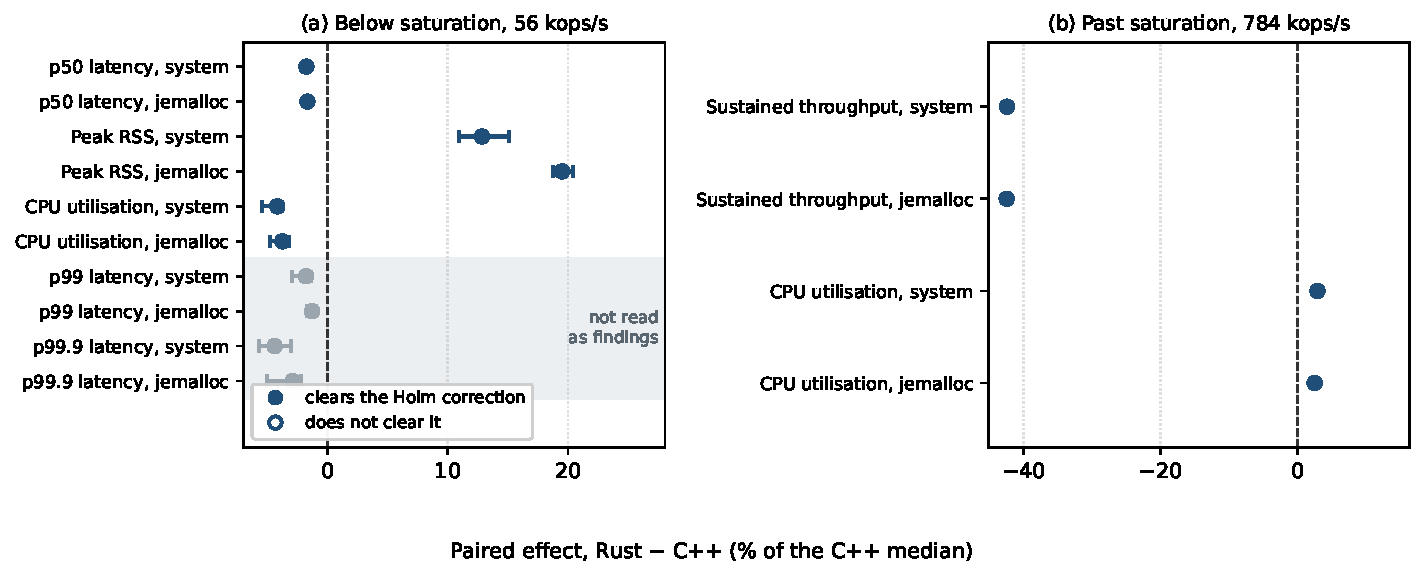
\includegraphics[width=0.78\linewidth]{figures/fig_effects.pdf}
\caption[The tested family drawn as paired effects]{Every test in Tables~\ref{tab:significance} and~\ref{tab:overloadtest} as a paired
effect with its bootstrap $95\%$ interval, normalised by the C++ median so that microseconds,
mebibytes, percentage points and kops/s can share an axis. Filled markers are the
\NSignificant{} of \NTests{} tests that clear the Holm correction, which on this host is all of
them. The two allocators of a
metric are drawn adjacent, so an effect that reversed sign between them would appear as a pair
straddling the zero line. The shaded rows are the high percentiles, computed from exactly the
operations interference falls on, which Section~\ref{sec:stats} fixes in advance as rows whose
\emph{intervals} are not read as findings. Their corrected $p$-values are read, and the shading
marks the instrument that is set aside rather than the rows. The metrics keep their own units in the
tables.\label{fig:effects}}
\end{figure}

Figure~\ref{fig:effects} draws the same family on one axis, and three things it contains are
easier to see there than in a table of fourteen rows: that every effect survives the correction,
that no effect changes sign when the allocator changes, and how much wider the tail
intervals are than the rest.

All \NSignificant{} of the \NTests{} tests in the family survive the Holm correction, and the
smallest adjusted value sits at the family's own floor of $\CorrectedFloor$. A family in which
nothing fails invites one obvious objection, that the threshold is doing no work, so it is worth
naming what would have failed. Peak resident set size under \texttt{jemalloc} did not clear the
correction on the virtualised host, despite an interval nowhere near zero, and
Section~\ref{sec:resources} takes up why it does here. Neither did any tail row.

The reading rule fixed in Section~\ref{sec:stats} still applies, and on this host it changes no
verdict. \NExclZero{} paired intervals exclude zero, in both blocks. Fixing the rule in advance, and
not at this point, was the whole precaution, because that outcome was not guaranteed: an earlier
seven-repeat pass of this same campaign produced tail intervals excluding zero, and more repeats then
removed them again. A rule kept only while it rescues a result is not a rule, so the tail block's
intervals are still not read as findings even though they now point the same way as its $p$-values.

The allocator control supplies a second check, independent of the first. Every comparison is run
twice under conditions that should not change a language effect, so an effect that really is the
language ought to keep its sign whichever allocator is linked. Here \CrossAllocConsistent{} all
do, and \NCrossAllocReversed{} reverse. That the control confirmed here and did not veto is no
evidence it was unnecessary. Section~\ref{sec:threats} records the earlier campaign on which it
did veto, and a control earns its place by what it would have caught.

Resolving a difference is not the same as sizing it, and Table~\ref{tab:equivalence} is where the
size goes. Every row is significant here, so the verdict column carries no information and the
margins carry all of it: a resolved difference of a microsecond and a resolved difference of a
millisecond mean quite different things to a deployment. At the median the effect could be no larger
than $\EqvBoundPFifty\,\mu$s, and in the tail block no larger than $\EqvBoundTailMax\,\mu$s. Both are
below anything a procedure budget of a few milliseconds would notice, which is the useful form of
this result: the differences are real, reproducible, and operationally negligible. That table was
built to report the opposite case, and on the virtualised host it did, with
\GuestNEqvUnresolved{} of its \GuestNTests{} rows unresolved and a tail margin running out to
$\GuestEqvBoundTailMax\,\mu$s, which is wider than any difference a deployment would care about and
was the campaign declining to answer.

\begin{table}[tp]
\centering
\small
\caption[How large each effect could be]{How large each effect could be. For every comparison at
$\ReprLoad$~kops/s, the observed effect against the tightest margin within which the two variants
could be called equivalent, and the verdict Table~\ref{tab:significance} reaches. The two
questions are kept in separate tables on purpose: one asks whether a difference is there, this one
asks how large it could be, and a row can matter in one and not the other. On the host reported
here every row resolves, so the last column reads the same throughout and the margins are what
carry the information: a resolved difference of a microsecond and a resolved difference of a
millisecond mean different things to a deployment. On the virtualised host of
Section~\ref{sec:hostcompare} \GuestNEqvUnresolved{} of these rows did not resolve, which is what the
table was built to report. Latency margins are in microseconds, peak resident set size in mebibytes,
CPU utilisation in percentage points.\label{tab:equivalence}}
\begin{tabular}{@{}l l r r l@{}}
\hline\hline
Metric & Allocator & $|$Effect$|$ & Equivalent within & Verdict \\
\hline
p50 latency (\textmu s) & system & 1.2 & 1.3 & significant \\
p50 latency (\textmu s) & jemalloc & 1.5 & 1.6 & significant \\
p99 latency (\textmu s) & system & 2 & 2 & significant \\
p99 latency (\textmu s) & jemalloc & 1 & 1 & significant \\
p99.9 latency (\textmu s) & system & 4 & 4 & significant \\
p99.9 latency (\textmu s) & jemalloc & 3 & 3 & significant \\
Peak RSS (MiB) & system & 1.6 & 1.8 & significant \\
Peak RSS (MiB) & jemalloc & 2.5 & 2.5 & significant \\
CPU utilisation (\%) & system & 6.0 & 7.1 & significant \\
CPU utilisation (\%) & jemalloc & 6.2 & 7.3 & significant
\\
\hline
\end{tabular}
\end{table}

The median itself is a resolved difference and not a null: $\PFiftyDiffAbsMax\,\mu$s
in Rust's favour, consistent under both allocators. The interval on it reaches
$\PFiftyDiffCIMax\,\mu$s against a median of $\PFiftyMedian\,\mu$s, and the temptation is to report
that as a bound on the language effect. That reading would be wrong, for the reason set out
next.

\paragraph{What the end-to-end number is made of.}\label{sec:budget}
Every latency the sweep reports is an end-to-end round-trip, and
Section~\ref{sec:methodperf} set out why that bundles two costs of quite different character: the
operation itself, executed inside a single thread and generated by the compiler, and the
cross-thread submit-and-complete handoff around it, charged to the operating system. Only the
first can plausibly differ between the languages, and the sweep cannot separate the two.

That matters for the bound just quoted, because a bound says only as much as the quantity
it is a fraction of. Both costs are therefore measured directly by the two-level method described
there, in both languages and at the sweep's own shard count and context population.
\texttt{ShardCore} with no queue in the path gives the operation, \texttt{Service} gives the
operation plus the handoff, and their difference is the handoff.
Table~\ref{tab:budget} gives the result, and it reframes the whole performance comparison.

\begin{table}[tp]
\centering
\small
\caption[Where an end-to-end operation's cost actually goes]{Where an end-to-end operation's cost actually goes, measured at $7$ shards and
$5\,000$ active UEs with a single uncontended caller. Each row is the median over
\BudgetRepeats{} interleaved repeats above its bootstrap $95\%$ confidence interval, in the
unit its own magnitude calls for: the two terms differ by more than two orders of magnitude,
which is the point of the table. $p$ is the exact two-sided paired permutation test of C++
against Rust on the repeat-wise differences. The handoff is obtained as the difference between
the two measured rows, so it carries the uncertainty of both.\label{tab:budget}}
\begin{tabular}{@{}l r r r@{}}
\hline\hline
Component & C++ & Rust & $p$ \\
\hline
Operation alone, no queue in the path (ns) & \mci{34.4}{32.5}{34.5} & \mci{21.3}{21.0}{22.5} & 0.000061 \\
Cross-thread submit-and-complete handoff (\textmu s) & \mci{13.49}{13.36}{13.64} & \mci{12.61}{12.37}{12.89} & 0.227 \\
End-to-end round-trip, uncontended (\textmu s) & \mci{13.52}{13.39}{13.68} & \mci{12.63}{12.39}{12.91} & 0.215 \\
Operation's share of the round-trip & 0.250\,\% & 0.170\,\% & 
\\
\hline
\end{tabular}
\end{table}

The operation is $\BudgetCoreCpp$~ns in C++ and $\BudgetCoreRust$~ns in Rust. The handoff is
$\BudgetHandoffCpp\,\mu$s and $\BudgetHandoffRust\,\mu$s. The work the languages actually
perform is therefore at most $\BudgetCoreShareMax\%$ of what the sweep measures. The
complementary $\BudgetCoreShareRest\%$ of every latency in Table~\ref{tab:latency} is the
operating system moving a message between two threads.

That shape is not peculiar to this system or to this pair of languages. On a shared-nothing
database partitioned one per worker thread like this service, Zhou et al.\ report that once the
per-operation work is optimised what dominates the rest is communication across isolation
boundaries and not the operation~\cite{zhou2025oltp}. The result below is therefore a general
property of the design and not an artefact of this measurement.

Two conclusions follow, and they pull in opposite directions.

The first is that the sweep cannot bound the language effect, and the bound quoted above must
not be read as though it does. An interval of $\PFiftyDiffCIMax\,\mu$s on the paired median
difference is $\BudgetBoundVsCore$ times the operation's own cost, so a language effect could be
several hundred percent of the work being done and still sit comfortably inside it. What the sweep
does establish is weaker and still useful: neither language disturbs the
scheduler-dominated round-trip, which is what a deployment of this shape would actually
experience. The limit comes from how the measurement is built and not from the host, so unlike
the tail result it will not be fixed by moving to bare metal. It is fixed by measuring the
component on its own, which is what this decomposition does.

The second is that once the component \emph{is} measured on its own, the languages are not
equivalent. \BudgetCoreFaster{} runs the bare operation about $\BudgetCoreRatio\times$ faster,
the difference shows up in the great majority of repeats, and the paired test puts it two
orders of magnitude below the conventional threshold. This decomposition is a separate
experiment from the sweep and no part of its Holm family. It runs \BudgetRepeats{} repeats
instead of \NRepeats{}, so its own attainable floor is $\BudgetFloor$ and not the
$\CorrectedFloor$ quoted in Section~\ref{sec:stats}, and no correction is applied to it. The
same holds for the interoperability comparison of Section~\ref{sec:migrationresults}. This is
the only place in the whole performance campaign where a
language difference in \emph{time} is resolved at all, and the sweep is blind to it by more
than two orders of magnitude.

Figure~\ref{fig:budget} draws both conclusions on one page, and its second panel is the argument
in one image: the instrument sits entirely above the quantity it would have to constrain.

\begin{figure}[ht]
\centering
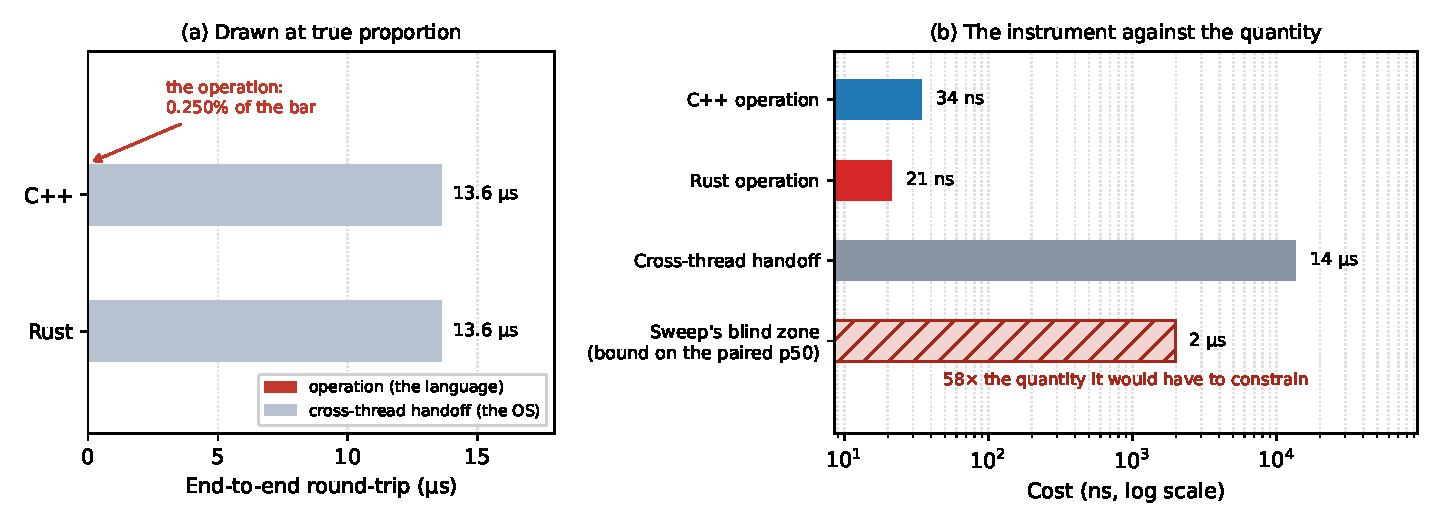
\includegraphics[width=0.78\linewidth]{figures/fig_budget.pdf}
\caption[The end-to-end operation decomposed, against what the sweep can resolve]{Where an end-to-end operation's cost goes, and why the sweep cannot bound a language
effect. \textbf{(a)} The round-trip at true proportion: the operation the language performs is
$\BudgetCoreShareMax\%$ of the bar, the remainder the cross-thread handoff. \textbf{(b)} The
same quantities on a log axis against the smallest paired difference the sweep can resolve,
shown as a blind zone. Both operation measurements fall inside it by a factor of
$\BudgetBoundVsCore$, and (b) is also where the sweep's one resolved language difference in time
lives.\label{fig:budget}}
\end{figure}

The attribution needs care, because the obvious reading is the wrong one. Nothing here
implicates the borrow checker, bounds checking, or ownership. The most likely source is
already recorded in the forced-idiom log of Table~\ref{tab:idioms}. The per-shard container is
each language's standard hash map, and those are different data structures. C++'s
\texttt{std::unordered\_map} has to be node-based to keep its iterator- and reference-stability
guarantees, so a lookup chases a pointer out of the bucket array into a separately allocated
node. Rust's \texttt{HashMap} is an open-addressed table that keeps entries inline and
usually resolves a lookup within one cache line. The hash function is pinned to FNV-1a on both
sides (Section~\ref{sec:impldetails}) precisely so that hashing could not be the explanation,
which leaves the container layout. That is a real and reportable difference between the two
languages as they are actually used, because a developer reaching for the standard hash map gets
whichever one their language ships. It is not evidence about Rust's safety model and should
not be quoted as such. Confirming the mechanism would need the cache-miss counters
Section~\ref{sec:threats} lists as the clearest instrumentation gap.

Two limits keep the finding the size it is. It is a single-threaded, uncontended
microbenchmark, so it says what the operation costs and not what a loaded system does with it, and
it is one operation on one data structure. Generalising from it to ``Rust is
$\BudgetCoreRatio\times$ faster'' would repeat exactly the error this thesis criticises in the
average-case literature.

\paragraph{Latency, throughput and the knee across the sweep.}
Figure~\ref{fig:loadsweep}(a) plots p99 latency against offered load, and the shape it shows is
the one Figure~\ref{fig:cliff} sketched, with one feature sharper than the sketch. Through the whole
tracking region p99 is \emph{flat}: it reads $\PNineNineLightest\,\mu$s at the lightest load and
$\PNineNineTrackingTop\,\mu$s at the top of the region, a drift of
$\PNineNineTrackingDrift\,\mu$s across a fifty-fold increase in offered load. A queueing model would
predict a gentle climb, and there is none to see, because until a worker saturates its shard the
queue never holds more than a request or two and latency is service time rather than waiting time.
Then, in the single step of the rate ladder that follows, p99 rises by four orders of magnitude at
once, from $\PNineNineTrackingTop\,\mu$s to seconds. That is the overload cliff, and how abruptly it
arrives is the finding. One increment of offered load separates a service meeting millisecond
deadlines from one missing them by three orders of magnitude. A design with bounded, blocking queues
has no graceful degradation to offer in between, and the flatness before the cliff is why: there is
no rising-latency region to warn an operator that capacity is close.

Section~\ref{sec:stats} tests no percentile past the knee, for two reasons. Latency there is
accumulated schedule backlog and not service time, and the measured phase is cut off at a fixed
width, so the reported percentiles saturate near it and every one above the knee is a lower bound.
What stays interpretable is how much work each variant still completes, which
Section~\ref{sec:overload} takes up.

Panel~(b) shows achieved throughput against the same axis, and it is the
more informative of the two, because an average over a whole run is far less sensitive than
a percentile to interference landing on individual operations. All four variants track the ideal
offered-equals-achieved line up to an offered $\TrackingLoad$~kops/s, and the lowest plateau any of
them reaches is $\SatKnee$~kops/s. Each knee is bracketed by the rate ladder and not pinned by it:
the next rung is where an arm stops tracking, so its true saturation point lies between the two and
the sweep steps over it. Achieved throughput matches offered load below the knee to within
$\ReprLoadShortfall\%$, so the operating point of Table~\ref{tab:latency} is a genuinely
\emph{sustained} load and not a nominal one, and the latencies reported there are not those of an
already-queueing system.

The knee does \emph{not} sit at the same place for all four variants, and that is worth stating
plainly because the identical thread-per-shard structure predicts that it should. The two C++ arms
stop meeting their offered rate after $\TrackingLoadCpp$~kops/s and the two Rust arms carry one rung
further, to $\TrackingLoadRust$. The separation is by language and not by allocator, as it is
everywhere else in this regime. At the rung between the two limits, $\KneeGapLoad$~kops/s, the
consequence is the largest throughput gap anywhere in the sweep: \KneeGapFaster{} still serves
$\KneeGapThrFast$~kops/s while \KneeGapSlower{} has already collapsed to $\KneeGapThrSlow$, a factor
of $\KneeGapRatio$, in \KneeGapAgree{} paired repeats.

Three things bound what that rung licenses, and the first is a rule this study set for itself. It is
\emph{not} added to the tested family of Section~\ref{sec:stats}. The operating point was identified
after seeing the sweep, and the family is fixed in advance precisely so that a point chosen that way
cannot enter it, whatever its $p$-value would be. It is therefore reported descriptively, with its
per-repeat agreement, and the pre-committed overload point of Section~\ref{sec:overload} stands as
the tested comparison. Second, one rung of a geometric ladder is coarse: the true C++ limit lies
somewhere between $\TrackingLoadCpp$ and $\KneeGapLoad$~kops/s, so the gap in \emph{capacity} is
bounded by the ladder's spacing and is not measured to better than that. Third, the direction here is
the opposite of the direction past saturation, where C++ sustains more
(Section~\ref{sec:overload}). Both are real, they belong to different loads, and neither cancels the
other. The useful summary is that the two languages differ in \emph{where} this design stops coping
and in \emph{how} it behaves once both have, and they differ in opposite directions.

\begin{figure}[ht]
\centering
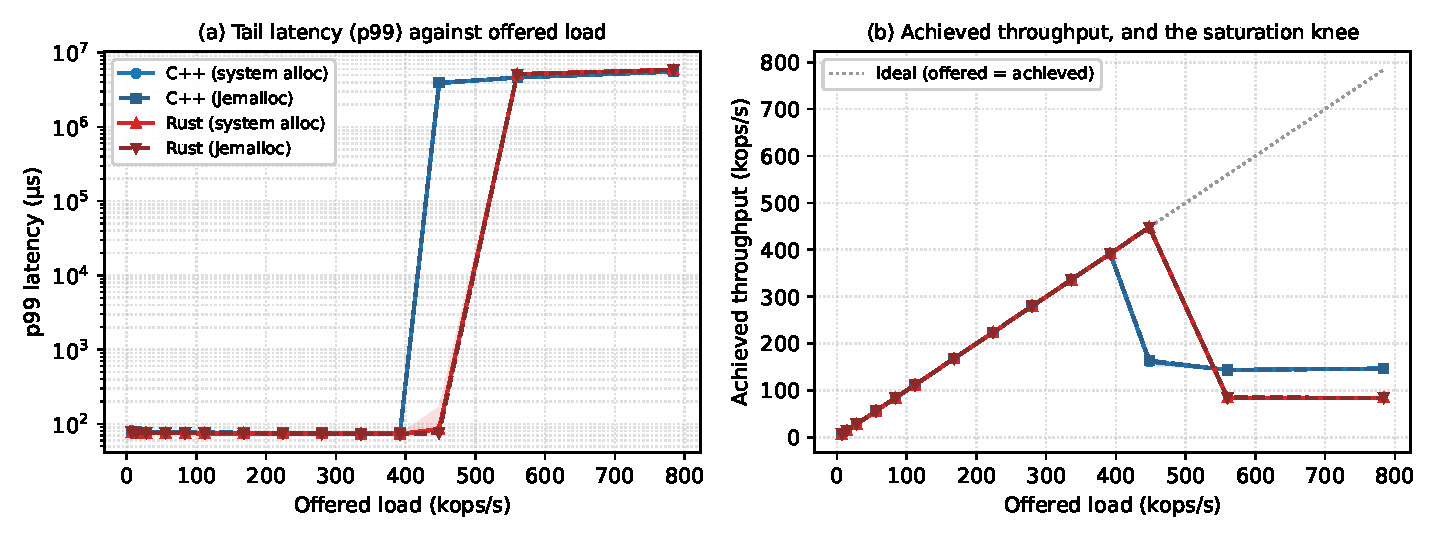
\includegraphics[width=0.78\linewidth]{figures/fig_load_sweep.pdf}
\caption[The load sweep: tail latency and achieved throughput]{The load sweep, both panels
against offered load. \textbf{(a)} Tail latency (p99) for the four build variants on a log axis. It
is flat across the whole tracking region and then rises by four orders of magnitude in one step of
the ladder. \textbf{(b)} Achieved throughput, with the dotted line marking the ideal
offered-equals-achieved regime. The C++ curves leave that line after an offered
$\TrackingLoadCpp$~kops/s and the Rust curves after $\TrackingLoadRust$, which is the one place in
the sweep where the two languages part company below the deepest overload. Lines are medians over
\NRepeats{} repeats and shaded bands are bootstrap $95\%$ confidence intervals in both panels,
which share the variant styling of the legend in (a). Throughput is counted over the measured
phase only, so the warm-up iterations bias neither the numerator nor the
denominator.\label{fig:loadsweep}}
\end{figure}

Figure~\ref{fig:tailpct} holds the load fixed instead and sweeps the percentile. The four
variants coincide at the median and fan out as the percentile rises. That is the expected shape
for a heavy-tailed distribution, and it is why a percentile-aware methodology is used throughout.
The fanning is not a language effect. Its right-hand panel sets the spread between the four
variants against the widest interval on any one of them, and from p90 upward the interval wins,
so the fan marks where the measurement loses resolution and not where the languages differ.

\begin{figure}[ht]
\centering
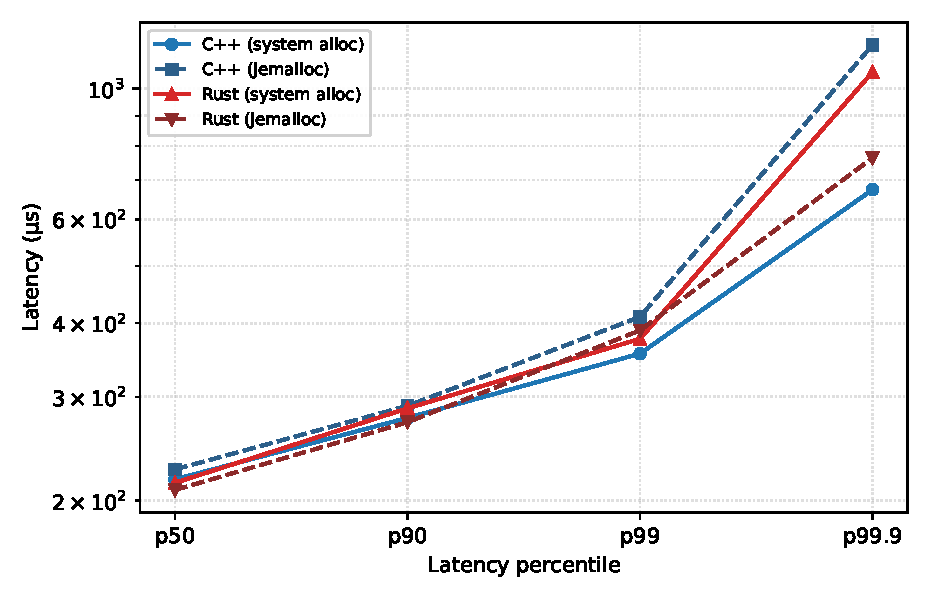
\includegraphics[width=0.78\linewidth]{figures/fig_tail_percentiles.pdf}
\caption[Latency across the percentile range, and the limit of the host]{Per-operation latency across the percentile range at $\ReprLoad$~kops/s. \textbf{(a)} The
four variants as medians over \NRepeats{} repeats, each with a bootstrap $95\%$ band. The bands
are the point: drawn as bare lines the curves lie on top of one another and read as a claim of
equivalence, which is not what a measurement that cannot separate them has shown. \textbf{(b)}
Why they cannot be separated above the median. The spread between the four variants is set
against the widest confidence interval on any one of them, with the ratio annotated above each
pair of bars. Once that ratio passes one, the uncertainty about a single variant is larger than
the gap between all four and no ordering can be read off.\label{fig:tailpct}}
\end{figure}

\subsection{Past saturation (RQ1)}\label{sec:overload}
RQ1 asks how the two languages compare under increasing load \emph{and overload}, and everything
reported so far has been below the knee. This section is the other half. The operating point is
$\OverloadLoad$~kops/s offered, defined as the deepest swept load at which every variant has
stopped meeting the offered rate, and the metrics are the two that remain interpretable there
(Section~\ref{sec:stats}). Table~\ref{tab:overload} gives what each variant still sustains and
Table~\ref{tab:overloadtest} tests the comparison.

The languages are not equivalent in this regime, and the margin is not marginal.
\OverloadSustainedFaster{} sustains $\OverloadThrCpp$~kops/s where \OverloadSustainedSlower{}
sustains $\OverloadThrRust$, a factor of $\OverloadThrRatio$. The paired difference is at least
$\OverloadThrBound$~kops/s under either allocator, it holds in \OverloadThrAgree{} repeats, and
its Holm-adjusted $p$ sits at the corrected floor of the whole family of \NTests{} tests. This is
the largest language effect in the tested family and the most reproducible effect in the study.
One larger ratio appears in the sweep, at the rung between the two languages' saturation limits
(Section~\ref{sec:perfresults}), and it runs the other way and is not tested, for the reason given
there.

The CPU column rules out the reading that would otherwise be natural, that a variant completing
less work is simply doing less, whether throttled, blocked or idle. That is not what happens.
\OverloadSustainedSlower{} draws \emph{more} total CPU than \OverloadSustainedFaster{} here,
reproducibly and under both allocators, having flipped the sign it carried at the representative
load in Table~\ref{tab:significance}. Divided through by the work that actually completed, its
CPU cost per sustained operation is $\OverloadCpuPerOpRatio$ times the other's. Neither
variant is near the capacity of the machine either, since both sit near six of the
$\MainPinnedCount$ pinned
cores. So the gap is not a capacity limit and not idleness. It is effort spent without completing
operations, which is the signature of a synchronisation path that spins, or parks and
wakes repeatedly, where the other blocks once and sleeps.

Figure~\ref{fig:overload} puts both halves of that reading side by side, and its grouping adds a
third: the separation falls almost entirely inside the allocator groups, so the effect
follows the variable the study manipulates and not the one it controls for.

\begin{figure}[ht]
\centering
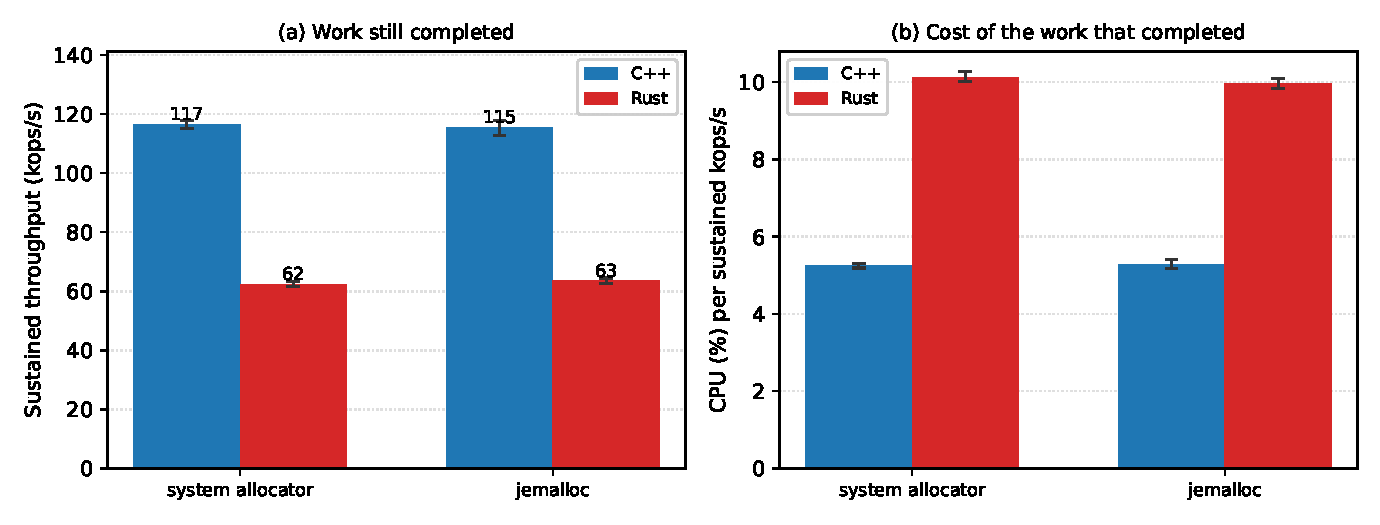
\includegraphics[width=0.78\linewidth]{figures/fig_overload.pdf}
\caption[Divergence past saturation]{Behaviour at $\OverloadLoad$~kops/s offered, well beyond the $\SatKnee$~kops/s knee. Bars
are medians over \NRepeats{} repeats with bootstrap $95\%$ intervals, grouped so that the two
bars inside a group differ only in language. \textbf{(a)} What each variant still completes:
\OverloadSustainedFaster{} sustains a factor of $\OverloadThrRatio$ more than
\OverloadSustainedSlower. \textbf{(b)} Total CPU divided by the work that actually completed,
which is what rules out the reading that the variant delivering less is simply doing less. It
spends $\OverloadCpuPerOpRatio$ times as much CPU per sustained operation, and the CPU figures
are summed across threads.\label{fig:overload}}
\end{figure}

Where that effort goes is narrowed by measurement. Past
saturation the producers spend almost all their time in two places recorded in
Table~\ref{tab:idioms}: the bounded blocking queue and the completion handle. The microbenchmark
below isolates those primitives, and they do not reproduce the
full-service ordering at significance. That rules them out \emph{alone} as the whole explanation
for a $\OverloadThrRatio\times$ gap. As in Section~\ref{sec:budget}, nothing in the safety model
is implicated.

The setting bounds what the finding licenses, and Section~\ref{sec:threats} says how far it
travels. The depth of the collapse depends on one design, one request outstanding per producer and
a queue bound of $1\,024$, measured with a harness whose producers block per request. What travels
is the ordering and its cause: below saturation the language choice did not matter, and above it
the standard library's synchronisation primitives did.

The closest prior work reports a comparable degradation past a threshold request rate and
attributes it to the asynchronous runtime~\cite{arvidsson2025async}.
Section~\ref{sec:rqdiscussion} takes up what it means that the same shape appeared here with no
such runtime on either side.

\begin{table}[H]
\centering
\small
\caption[What each variant sustains past saturation]{What each variant still sustains at
$\OverloadLoad$~kops/s offered, well beyond the $\SatKnee$~kops/s knee: the median over
\NRepeats{} repeats above its bootstrap $95\%$ confidence interval. Below saturation achieved
throughput is pinned to the offered rate by construction and can express nothing about the
languages. Here it is the only thing that can. CPU utilisation exceeds $100\%$ because it is
summed across threads, so $600\%$ is six busy cores of the $\MainPinnedCount$
pinned.\label{tab:overload}}
\begin{tabular}{@{}l r r@{}}
\hline\hline
Variant & sustained throughput (kops/s) & CPU (\%) \\
\hline
C++ (system alloc) & \mci{146.7}{146.3}{147.2} & \mci{662.8}{662.5}{663.6} \\
C++ (jemalloc) & \mci{146.4}{146.1}{146.9} & \mci{664.3}{663.3}{664.9} \\
Rust (system alloc) & \mci{84.5}{84.2}{84.7} & \mci{681.8}{680.4}{682.5} \\
Rust (jemalloc) & \mci{84.3}{83.9}{84.6} & \mci{680.3}{679.8}{681.5}
\\
\hline
\end{tabular}
\end{table}

\begin{table}[H]
\centering
\small
\caption[Exact paired test past saturation]{Exact paired permutation test of C++ against Rust at
$\OverloadLoad$~kops/s, the allocator held fixed, Holm-corrected across the same family of
\NTests{} tests as Table~\ref{tab:significance} rather than as a family of its own. ``Repeats''
counts how many of the \NRepeats{} paired differences agree with the sign of the median, which a
statistic computed from their mean cannot show. No latency percentile is tested here, for the
reason fixed in advance in Section~\ref{sec:stats}.\label{tab:overloadtest}}
% The generated metric names are long enough that six l/r columns overrun the text
% block; the first column wraps instead, and the inter-column padding is tightened.
\setlength{\tabcolsep}{4pt}
\begin{tabular}{@{}p{0.24\linewidth} l r c r r@{}}
\hline\hline
Metric & Allocator & Effect (Rust $-$ C++) & Repeats & $p$ & Holm \\
\hline
Sustained throughput (kops/s) & system & \mci{-62.2}{-62.9}{-61.6} & 20/20 & 0.0000019 & 0.000027 \\
Sustained throughput (kops/s) & jemalloc & \mci{-62.2}{-62.7}{-61.6} & 20/20 & 0.0000019 & 0.000027 \\
CPU utilisation (\%) & system & \mci{+19.5}{+17.3}{+19.9} & 20/20 & 0.0000019 & 0.000027 \\
CPU utilisation (\%) & jemalloc & \mci{+16.8}{+15.6}{+17.5} & 20/20 & 0.0000019 & 0.000027
\\
\hline
\end{tabular}
\end{table}

\paragraph{The contended queue and completion primitives on their own.}\label{sec:contention}
The overload result attributes its gap to the two forced-idiom synchronisation constructs, but
that attribution was argued from the shape of the full-service measurement. A microbenchmark
isolates those constructs alone.

\ContentionProducers{} producer threads hammer one bounded queue of capacity $1\,024$ while a
single consumer drains it. Each producer submits a no-op job carrying a one-shot completion handle and blocks
until the consumer signals. No \texttt{ShardCore} work runs in the path. C++ uses the
hand-written \texttt{BoundedQueue} of Section~\ref{sec:impldetails} with
\texttt{std::promise}/\texttt{std::future}. Rust uses \texttt{sync\_channel} and a fresh
\texttt{mpsc::channel()} per request. Each timed window lasts two seconds after a warmup.
\ContentionRepeats{} interleaved repeats are summarised as medians with bootstrap intervals and
tested with the exact paired permutation procedure of Section~\ref{sec:stats}.
Table~\ref{tab:contention} reports the result.

\begin{table}[tp]
\centering
\small
\caption[Throughput through the contended synchronisation primitives alone]{Throughput through
the bounded queue and completion primitives alone, with \ContentionProducers{} contending producers
and queue capacity $1\,024$. Values are medians over \ContentionRepeats{} interleaved repeats above
bootstrap $95\%$ confidence intervals. The paired test compares C++ against Rust on sustained
throughput (kops/s). Measured on the host of Section~\ref{sec:testbed}.\label{tab:contention}}
\begin{tabular}{@{}l r r r@{}}
\hline\hline
Language & Throughput (kops/s) & Mean ns/op & Paired $p$ \\
\hline
C++ & \mci{55.0}{53.7}{58.4} & \mci{18178}{17110}{18632} & \multicolumn{1}{c}{---} \\
Rust & \mci{58.7}{56.8}{61.8} & \mci{17045}{16169}{17594} & 0.226
\\
\hline
\end{tabular}
\end{table}

The isolated primitives do not reproduce the overload ordering. C++ sustains
\ContentionThrCpp{}~kops/s and Rust \ContentionThrRust{}~kops/s, a gap of only
$\ContentionRatio\times$ with $p = \ContentionP$, where the full service at
$\OverloadLoad$~kops/s separates by $\OverloadThrRatio\times$ with its corrected $p$ at the
family floor. So the overload divergence involves extra work the microbenchmark strips away: the
larger tagged \texttt{Request} on the C++ side, the worker's variant dispatch, and the map
operations that still execute in the overload regime. An orders-of-magnitude difference in the
primitives alone is ruled out, which moves the search for the mechanism to the rest of the handoff
path and not to the safety model.

\subsection{Resource use (RQ3)}\label{sec:resources}
Table~\ref{tab:resource} reports resource use at the same
sustained load. Peak resident set size separates the two \emph{languages} cleanly, and it does so
whichever way the family is read: its paired intervals exclude zero, its effect keeps its sign under
both allocators, and both rows clear the correction. It does not separate all four variants, because
the C++ build with \texttt{jemalloc} and the Rust build with the system allocator land on the same
footprint from opposite directions, which is the arithmetic of two comparable effects and is the
subject of the next paragraph. Figure~\ref{fig:resources} plots the same measurement, and its middle
panel is where the finding of this section sits.

Two effects are present in it, not one, and they are of comparable size. Linking
\texttt{jemalloc} costs $\RssAllocDiffLo$--$\RssAllocDiffHi$~MiB in either language. The Rust
build costs $\RssLangDiffLo$--$\RssLangDiffHi$~MiB more than the C++ build under either allocator,
with a bootstrap interval of $\RssLangCILo$ to $\RssLangCIHi$~MiB. Resource use follows both, and
neither dominates the other. Part of the allocator figure comes from the fairness controls rather
than from \texttt{jemalloc} in general: both builds pin the arena count identically, so that
neither language's default could become an accidental advantage, and pinning it high makes the
arena metadata a fixed cost on both sides. A deployment tuning \texttt{jemalloc} for footprint
instead of for comparability would not pay it.

The relative size of these two effects is the one result in this chapter that a change of host
overturned. On the virtualised machine this study used first, the allocator effect measured
$\GuestRssAllocLo$--$\GuestRssAllocHi$~MiB, about $\GuestRssAllocOverLang$ times the language
effect rather than comparable to it, and the language effect was the same size there as here.
Section~\ref{sec:hostcompare} reports the comparison and what can and cannot be concluded from it.
The lesson for reading this paragraph is narrow and worth stating: the \emph{language} effect on
peak RSS is reproducible across three machines, and the \emph{allocator} effect is not a constant
of the allocators.

Every row in the upper block of Table~\ref{tab:significance} now clears the correction, including
peak RSS under \texttt{jemalloc}, which did not on the previous host. That row failed there for a
reason in the statistic rather than in the software: a handful of runs reported a resident set some
$\GuestRssLowRunOffset$~MiB low, and a permutation statistic built on a mean of paired differences
is dominated by them. The same measurement on this host spreads by $\RssLowRunOffset$~MiB, so the
contamination was the machine's. The rule fixed in advance in Section~\ref{sec:stats} for reading
such a row against its interval was not needed here, and it stays stated because a design that only
declares its reading rules when they rescue a result is not applying them.

CPU utilisation behaves differently again, and by regime rather than by noise.
At this below-saturation operating point Rust draws slightly \emph{less} CPU, by
at most $\CpuDiffAbsMax$ percentage points, consistently under both allocators and clearing the
correction under both. Section~\ref{sec:overload} finds the sign flipped past saturation and the
magnitude much larger. Achieved throughput adds nothing here, for the reason
Section~\ref{sec:stats} gives. At a below-saturation point it is pinned to the offered load, and
it is reported only to confirm that the point is sustained and not merely nominal, which it is to
within $\ReprLoadShortfall\%$.

The finding is a difference in fixed cost and not in cost per context. At the $\SweepUes$ active
UEs used in the sweep, the $\UeCtxGapBytes$-byte layout difference measured in
Section~\ref{sec:uecontext} accounts for roughly $\UeCtxGapTotalKB$~kB, two orders of magnitude
short of the gap, so most of it is runtime and allocator-arena overhead, which does not scale with
the workload and would matter proportionally less in a larger deployment. That is an argument from
elimination and this campaign cannot do better, because it reads the resident set only through
\texttt{getrusage}. Section~\ref{sec:baremetal} reads the allocator's own accounting on a host that
also exposes hardware counters, and decomposes the same gap directly.

The RQ3 finding is therefore neither the flat ``no resource penalty'' that overlapping intervals
would suggest nor a general one. Rust costs a few megabytes more of fixed footprint under both
allocators, comparable to what the allocator choice costs here though not on every host measured
(Section~\ref{sec:hostcompare}), and its CPU cost changes sign with the load regime.

\begin{table}[H]
\centering
\small
\caption[Resource use at the representative load]{Resource use at a sustained offered load of $\ReprLoad$~kops/s: achieved throughput,
peak RSS, and total CPU utilisation. The median over \NRepeats{} repeats above its bootstrap
$95\%$ confidence interval. Peak RSS and CPU both separate the two languages here. Neither
separates all four variants, and peak RSS cannot, because the allocator effect and the language
effect are of comparable size and one middle pair therefore
coincides.\label{tab:resource}}
\begin{tabular}{@{}l r r r@{}}
\hline\hline
Variant & throughput (kops/s) & peak RSS (MiB) & CPU (\%) \\
\hline
C++ (system alloc) & \mci{27.99}{27.99}{27.99} & \mci{9.4}{9.4}{9.5} & \mci{66.8}{65.8}{68.2} \\
C++ (jemalloc) & \mci{27.95}{27.95}{27.96} & \mci{65.9}{65.9}{65.9} & \mci{64.6}{63.4}{66.1} \\
Rust (system alloc) & \mci{27.99}{27.99}{27.99} & \mci{11.2}{11.1}{11.3} & \mci{63.3}{62.2}{66.0} \\
Rust (jemalloc) & \mci{27.95}{27.92}{27.96} & \mci{67.2}{65.4}{67.3} & \mci{63.0}{62.4}{64.5}
\\
\hline
\end{tabular}
\end{table}

\begin{figure}[ht]
\centering
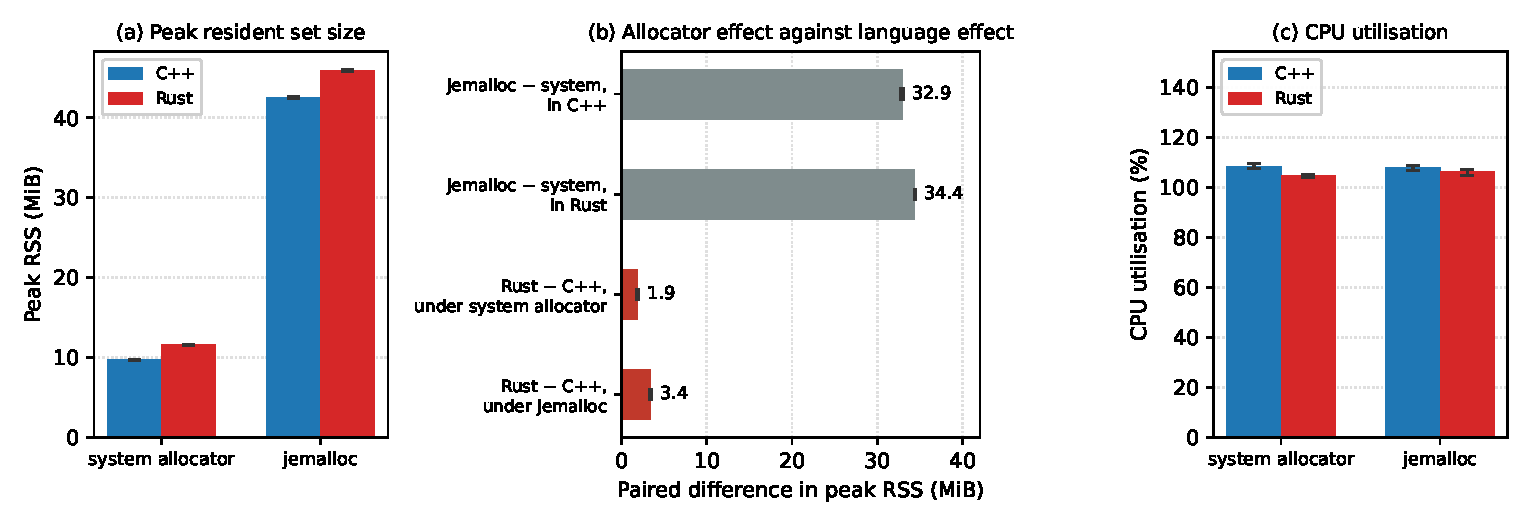
\includegraphics[width=0.78\linewidth]{figures/fig_resources.pdf}
\caption[Resource use, and the two effects inside peak RSS]{Resource use at a sustained offered load of $\ReprLoad$~kops/s, grouped by allocator so
that the two bars in a group differ only in language and the two groups differ only in allocator.
Medians over \NRepeats{} repeats with bootstrap $95\%$ intervals. \textbf{(a)} Peak resident set
size. \textbf{(b)} The two effects it contains, each as a paired difference over the same
repeats: linking \texttt{jemalloc} costs $\RssAllocDiffLo$--$\RssAllocDiffHi$~MiB, while the Rust
build costs $\RssLangDiffLo$--$\RssLangDiffHi$~MiB more than the C++ one. Both are real and on a
shared axis they are of comparable size, which was not true on the host this study used first
(Section~\ref{sec:hostcompare}). \textbf{(c)} CPU utilisation, summed across threads, where the
difference runs the other way and is small.\label{fig:resources}}
\end{figure}

\subsection{What the machine decided, and what the code decided}\label{sec:hostcompare}
\label{sec:baremetal}%
Every number above was measured on the bare-metal host of Section~\ref{sec:testbed}. For most of
this study they were measured on a virtualised one instead, at the same shard count, the same
fourteen load levels, the same \GuestRepeats{} repeats and the same toolchain. Two campaigns that
differ in the machine alone are an opportunity a single-host study does not get, and this section
takes it. The question is not which host is faster. It is which of this chapter's findings are
properties of the code and which were properties of the machine, because a comparative study that
cannot tell those apart is reporting its testbed.

\paragraph{The instrument, which is where the difference is largest.}
On the virtualised host the $95\%$ interval on one variant's own p99 spanned
$\GuestPNineNineMaxCI\,\mu$s while the four variants' p99 values differed by
$\GuestPNineNineRange\,\mu$s. Uncertainty about one variant exceeded the gap between all of them by
a factor of five, so no ordering could be read at that percentile however many repeats were run.
Computed identically here, the interval is $\PNineNineMaxCI\,\mu$s against a between-variant range
of $\PNineNineRange\,\mu$s. The relation inverts. That single change is what moves the far tail
from an open question to a reported result, and it is worth being precise about its cause. At the
same representative load the median barely moved, from $\GuestPFifty$ to $\PFiftyMedian\,\mu$s,
while p99 fell from $\GuestPNineNine\,\mu$s to under a hundred. A hypervisor does not slow the common
path. It
occasionally stops it, and a percentile computed from exactly the stopped operations is the one
that records it.

\paragraph{What survived the change of host.}
The overload divergence did, and it is the strongest claim in the chapter for that reason. The
ratio of sustained throughput past saturation was $\GuestOverloadThrRatio\times$ on the guest and
is $\OverloadThrRatio\times$ here, on another vendor's silicon, with the ordering unchanged. The
saturation knee moved as capacity should, from $\GuestSatKnee$ to $\SatKnee$~kops/s. The peak-RSS
\emph{language} effect survived too, at $\GuestRssLangLo$--$\GuestRssLangHi$~MiB there against
$\RssLangDiffLo$--$\RssLangDiffHi$~MiB here, which is the same effect within measurement error on
two machines, two vendors and two memory subsystems.

\paragraph{What did not survive, and this is the one to read carefully.}
The peak-RSS \emph{allocator} effect. On the guest, linking \texttt{jemalloc} cost
$\GuestRssAllocLo$--$\GuestRssAllocHi$~MiB, roughly $\GuestRssAllocOverLang$ times the language
effect, and while that host was the only evidence this thesis reported the gap as an order of
magnitude. Here the same comparison costs $\RssAllocDiffLo$--$\RssAllocDiffHi$~MiB, which is the
same size as the language effect rather than ten times it. The claim that the allocator dominates
the footprint was a property of that machine.

The mechanism is not established, and the honest form of the finding is the comparison rather than
an explanation of it. One host property is a candidate and is recorded in both captures: transparent
hugepages were set to \GuestThp{} on the guest and \MainThp{} here, and the campaign pins
\texttt{thp:never} for \texttt{jemalloc} while the system-allocator arm inherits whatever the kernel
does, so the two arms were not treated alike by a policy neither of them chose. This study did not
vary that policy with everything else held fixed, so it cannot attribute the difference to it. What
it can say is that a second bare-metal host at a different shard count measured
$\BmRssAllocLo$--$\BmRssAllocHi$~MiB, which agrees with the figure here and not with the guest's,
so the guest is the outlier of three rather than one reading of two.

A related artefact went with it. The run-to-run spread that cost peak RSS under \texttt{jemalloc}
its place in the significance family, a handful of runs reporting a resident set
$\GuestRssLowRunOffset$~MiB low, is $\RssLowRunOffset$~MiB here, its paired repeats agree on the
sign \RssAgree{} times, and \CrossAllocConsistent{} keep their sign across the allocator control.

\paragraph{A second bare-metal host, at a different design.}
One \BmCpu{}, \BmCores{} cores on \BmSockets{} socket and \BmNumaNodes{} NUMA node, running
\BmDistro{} with \texttt{g++~\BmGpp} and \texttt{rustc~\BmRustc}. The governor is fixed at
\BmGovernor{}, simultaneous multithreading is \BmSmt{}, and cores \BmPinned{} carry the
benchmark. The environment capture records virtualisation as \BmVirt{}. Across
\BmStealWindow{}~s of wall clock, \BmStealWithSteal{} of \BmStealIntervals{} sampling intervals
on the \BmStealCores{} pinned cores showed any CPU steal. The sweep is \BmRuns{} runs:
\BmRepeats{} repeats over \BmLoadLevels{} offered loads from \BmLoadLo{} to \BmLoadHi{}~kops/s,
four variants interleaved inside each repeat as before.

\paragraph{The far tail, measured twice.}
A percentile this far out is the one most likely to be an artefact of a single campaign's design, so
it is worth having two. Pooling this host's repeats gives \BmPoolSamplesMin{} to
\BmPoolSamplesMax{} operations per group, which is what makes p99.99 a measurement rather than a
handful of draws. Between \BmFarTailSepLoad{} and \BmFarTailSepHi{}~kops/s the pooled p99.99 of the
two C++ variants falls between $\BmFarTailCppLo$ and $\BmFarTailCppHi\,\mu$s and that of the two
Rust variants between $\BmFarTailRustLo$ and $\BmFarTailRustHi\,\mu$s, and the two ranges do not
meet. Below \BmFarTailSepLoad{}~kops/s the four are indistinguishable. The direction is the one the
main campaign reports, at a different shard count and a different load grid, which is the
strongest statement two campaigns can make jointly. The highest swept load is held out of both
statements, because its pooled median falls while every percentile above it stays flat and this
campaign does not explain that shape.

\paragraph{What survived the change of design.}
The median difference clears Holm correction at \BmPFiftySig{} of \BmPFiftyTested{}
load-and-allocator points, with \BmPFiftyFaster{} lower by
$\BmPFiftyDiffLo$--$\BmPFiftyDiffHi\,\mu$s on an operation of $\BmPFiftyMedian\,\mu$s. Peak RSS is
significant at \BmRssSig{} of \BmRssTested{} points, with the Rust build costing
$\BmRssLangLo$--$\BmRssLangHi$~MiB more than the C++ one and \texttt{jemalloc} costing
$\BmRssAllocLo$--$\BmRssAllocHi$~MiB more than the system allocator. Those two figures matter beyond
this section: they are of comparable size, they agree with the main campaign's, and they disagree
with the virtualised host's, which is the third of the three measurements
Section~\ref{sec:hostcompare} weighs against each other.
The CPU comparison below saturation is significant at \BmCpuSig{} of \BmCpuTested{} points with
\BmCpuLower{} lower at every one of them, by $\BmCpuDiffLo$--$\BmCpuDiffHi$ percentage points, the
gap widening with offered load.
The divergence past saturation reproduces here too. Every arm tracks its offered load to
\BmTrackingMax{}~kops/s and the knee falls between \BmKneeLo{} and \BmKneeHi{}~kops/s. At
\BmOverloadLoad{}~kops/s, where all four arms have collapsed and each one's repeats agree to within
$\BmOverloadCv\%$, \BmOverloadFaster{} sustains $\BmOverloadThrCpp$~kops/s against
$\BmOverloadThrRust$, a ratio of $\BmOverloadThrRatio$ against the $\OverloadThrRatio$ of
Section~\ref{sec:overload}. Three hosts and two shard counts now put that ratio between
$\BmOverloadThrRatio$ and $\GuestOverloadThrRatio$, always with the same arm ahead.
One load must not be quoted. At \BmMetastableLoad{}~kops/s, the first load past the knee, the
Rust arms are bimodal across repeats and their throughput varies by $\BmMetastableCv\%$, serving
the full offered rate in some repeats and collapsing in others. A median there would average a
distribution with a mode at each end.

\paragraph{A mechanism, from hardware counters.}
Section~\ref{sec:perfresults} attributes the operation-level difference to the forced idioms of
Table~\ref{tab:idioms} on the strength of an argument about container layout. Counters turn that
argument into a measurement, and no virtualised host in this study exposed them. Over
\BmCounterRepeats{} interleaved repeats at the operation scope, the Rust build retires
$\BmInstrDelta\%$ \BmInstrDeltaDir{} instructions than the C++ one ($p=\BmInstrDeltaP$) and
finishes in $\BmCycleDelta\%$ \BmCycleDeltaDir{} cycles ($p=\BmCycleDeltaP$), while missing cache
$\BmMissDelta\%$ \BmMissDeltaDir{} often per thousand instructions ($p=\BmMissDeltaP$). Less work
in fewer cycles is a mechanism for the operation-level result, and it replaces an argument from
structure with a measurement. It says nothing about the resident set, and the worse locality is not
evidence that it does: a larger footprint is a reason to miss cache more often, so the two are
related in the opposite direction. The footprint has its own instrument, one paragraph down.

\paragraph{The resident set, decomposed by the allocator that holds most of it.}
Section~\ref{sec:resources} establishes that the peak-RSS difference is a fixed cost by
elimination, since the measured struct layout accounts for orders of magnitude too little. Both
benches also read \texttt{jemalloc}'s own accounting, and every one of the \BmJeRuns{} runs on the
two \texttt{jemalloc} arms carries it, so the composition can be read instead of inferred.
Table~\ref{tab:resident} gives it. Three readings, in the order they change the claim.

The bookkeeping is where the allocator's own difference sits, and it is fixed: arena metadata costs
the Rust build $\BmJeMetadataDelta$~MiB more, and that figure moves by $\BmJeMetaDrift\%$ across the
whole swept range, so it is a constant of the process and not a function of the workload.
\BmJeLiveLower{} nonetheless holds \emph{less} live allocation, by $\BmJeAllocatedDelta$~MiB, which
settles one thing outright: the larger resident set is not more application data.

The second reading is the one that relocates the finding. The allocator's own resident bytes are
$\BmJeResidentDelta$~MiB \emph{lower} in the Rust build, while its peak resident set is
$\BmJeRssDelta$~MiB higher. Subtracting the two inside each run, the footprint outside the
allocator's mappings is $\BmJeOutsideCpp$~MiB for the C++ build against $\BmJeOutsideRust$ for the
Rust one, a difference of $\BmJeOutsideDelta$~MiB. So the language effect on peak RSS is not an
allocator effect at all. It is the standard library and runtime a Rust process carries before it
allocates anything, and the allocator comparison runs the other way and partly offsets it. One
caveat travels with that subtraction: peak RSS is a maximum over the run and the
\texttt{jemalloc} figures are sampled once, so the outside-mappings figure is an upper bound rather
than an exact quantity.

The third reading is a negative result about the guest. The measurement defect that cost peak RSS
under \texttt{jemalloc} its place in the virtualised campaign's significance family, a handful of
runs reporting a resident set $\GuestRssLowRunOffset$~MiB low, does not appear here: no arm's peak
RSS spans more than $\BmRssSpreadMax$~MiB across its repeats. That bimodality belonged to the host,
which is what the reading rule of Section~\ref{sec:stats} assumed without being able to show it.

\begin{table}[ht]
\centering
\small
\caption[The resident set decomposed by the allocator]{Where the peak resident set goes on the
second bare-metal host, from \texttt{jemalloc}'s own accounting in each of the \BmJeRuns{} runs of
the two \texttt{jemalloc} arms. Medians in MiB over the steady-state loads, with the paired language
difference in the last column. The two rows below the rule are the argument: the allocator holds
\emph{less} in the Rust build, and the process holds more, so the difference is outside the
allocator. The final row is the quantity the other rows decompose. The derived row is the median of
the per-run difference and not the difference of two medians, because the two figures it subtracts
come from one process at one moment, so the column does not sum
exactly.\label{tab:resident}}
\begin{tabular}{@{}l r r r@{}}
\hline\hline
Component & C++ & Rust & Difference \\
\hline
Live allocation (\texttt{allocated}) & 0.78 & 0.62 & $-0.16$ \\
In active pages (\texttt{active}) & 1.43 & 0.79 & $-0.64$ \\
Arena bookkeeping (\texttt{metadata}) & 4.19 & 6.26 & $+2.07$ \\
Resident in allocator mappings (\texttt{resident}) & 11.02 & 9.10 & $-1.92$ \\
\hline
Outside those mappings (derived) & 4.04 & 7.86 & $+3.82$ \\
Peak resident set (\texttt{getrusage}) & 15.08 & 16.82 & $+1.74$\\
\hline
\end{tabular}
\end{table}

\paragraph{The allocation profile, and what it cannot attribute.}
The visit also captured a matched pair of \texttt{jemalloc} heap profiles, taken to name the call
sites behind the resident-set difference the readings above locate. They do not name them, and the
reason belongs in the record because it is a property of the instrument rather than of either
language. Peak RSS in the profiled run is $\BmProfRssDelta$~MiB higher in the \BmProfRssHigher{}
build, where the campaign's own \texttt{jemalloc} arms put \BmProfCampaignHigher{} higher by
$\BmProfCampaignLo$--$\BmProfCampaignHi$~MiB at every load it swept. No effect can be attributed in
a configuration that reverses its sign.

Two departures from the campaign could explain that reversal, and a second profile separates them.
The first was the operating point: the profile above ran closed loop at
$\BmProfThroughput$~kops/s, past the plateau bracketed at $\BmKneeLo$--$\BmKneeHi$~kops/s rather
than below it. Repeating it at a swept load below saturation shrank the discrepancy by most of its
size and did not remove it, so the wrong regime was the larger part of the effect and not its
cause. What remains is the second departure, and it is the one that cannot be engineered away:
profiling requires an allocator built to sample every allocation and record a backtrace for it, so
the arm under profile is not the arm the campaign measured. An instrument that perturbs the
quantity it reports by more than the difference under test cannot attribute that difference,
whatever load it runs at. The dumps are also harder to read
than the method anticipated. Each symbolised profile puts almost all of its flat bytes on a frame
that allocates nothing, $\BmProfFlatCppPct\%$ on a deallocation symbol in the C++ arm and
$\BmProfFlatRustPct\%$ on the allocator's own backtrace routine in the Rust one, so only the
cumulative call paths remain and those name subsystems rather than sites.

Two results survive those limits. Both arms allocate $\BmProfHistCpp$~MiB for the latency histogram,
equal to the byte, which is the harness parity control of Section~\ref{sec:controls} working where
it can be checked directly. At the same point in each arm's allocation history, the first dump of
the series, the worker path holds $\BmProfWorkerRust$~MiB in the Rust build against
$\BmProfWorkerCpp$~MiB in the C++ one. That is the shape a table reserved in one block gives against
a map grown a node at a time, so the container difference Section~\ref{sec:budget} argues from the
forced-idiom log is visible in allocation as well as in latency. Attributing the footprint itself
would need a profile taken at a swept load, on a build whose peak RSS reproduces the campaign's
ordering, and that is work for a repeat visit rather than a reanalysis of these dumps.

\paragraph{Inter-operation jitter.}
Every run recorded inter-operation delay variation, between $\BmJitterSamplesMin$ and
$\BmJitterSamplesMax$ samples of it, and no research question asks for the metric, so it is
described here and not tested. Below the top load all four variants sit between
$\BmJitterPFiftyLo$ and $\BmJitterPFiftyHi\,\mu$s at the median and between
$\BmJitterPNineNineLo$ and $\BmJitterPNineNineHi\,\mu$s at p99. The widest gap between the four at
any single load is $\BmJitterSpreadMax\,\mu$s. At $\BmJitterTopLoad$~kops/s they move together to
$\BmJitterTopLo$--$\BmJitterTopHi\,\mu$s, at least $\BmJitterTopRatio$ times any value below it.
Jitter on this service separates the load regimes rather than the languages.

\paragraph{Why three datasets rather than one, and what each is for.}
The three campaigns are not interchangeable and the differences between them are what makes each
one useful. The reported sweep and the virtualised one share a design exactly and differ in the
machine, which is what allows the first half of this section to attribute a change to the hardware.
This second bare-metal campaign differs in the design as well: \BmShards{} shards and
\BmProducers{} producers against the $7$ of Table~\ref{tab:params}, \BmLoadLevels{} loads against
\NLoadLevels{}, \BmRepeats{} repeats against \NRepeats{}, and \texttt{g++~\BmGpp} with
\texttt{rustc~\BmRustc} against the versions Table~\ref{tab:testbed} records. Shard count is one of
the fairness controls of Section~\ref{sec:controls} and the repeat count sets the floor the exact
test can reach, so this campaign cannot stand in for the reported one. What it can do is ask
whether the findings depend on those choices, and the answer is that the direction of every one of
them survives a change of shard count, load grid, repeat count and compiler at once. The compiler
half is the only evidence in this study that separates either language from one implementation of it
(Section~\ref{sec:threats}).

Two caveats belong with this campaign's numbers, and Table~\ref{tab:testbed} carries the first row
by row. It met the protocol on virtualisation, steal, governor and multithreading, and not on
tickless operation: \texttt{nohz\_full} is \BmNohzFull{} here, where the reported sweep runs
tickless on its pinned cores. The second is that its resource figures were recorded with the jitter
sidecar enabled, which costs both languages the same and lifts both absolute footprints, so paired
differences travel between campaigns and absolute peak RSS does not.

\subsection{Safety via fault injection (RQ2)}\label{sec:safetyresults}
This study does not claim that Rust has no bugs. It injects the catalogue of
$\FaultClasses$ defects set out
in Table~\ref{tab:defectmap}, each as a small self-contained program
flavoured with the subsystem's domain so that it maps onto a plausible bug in the service. The
split into two groups is what the method of Section~\ref{sec:methodfaults} turns on: seven
classes from inside the region Rust claims to govern, and seven chosen precisely because safe
Rust is expected \emph{not} to prevent them. With the second group the study measures a boundary
instead of demonstrating a claim, and a case that unexpectedly compiled, or unexpectedly failed
to, surfaces against its recorded expectation instead of being absorbed into the conclusion.

\paragraph{Procedure.}
Each C++ defect is built and run under AddressSanitizer (ASan), ThreadSanitizer (TSan) and
UndefinedBehaviorSanitizer (UBSan), and the matching construct is written in safe Rust and
compiled. The third sanitiser is not a refinement of the other two but a separate axis. Signed
overflow is invisible to both ASan and TSan, so without its own column the integer-overflow class
would be recorded as undetected in C++ when in fact it is caught. No static analyser is
run, for the reason set out in Section~\ref{sec:methodfaults}, so the C++ columns of
Table~\ref{tab:taxonomy} report the tooling this study ran and not a ceiling on what C++ tooling
could achieve. Where the Rust program compiles, it is run under a bounded timeout and its
observable behaviour recorded, because ``it compiles'' alone would not establish whether the
defect survives into the running program.

\paragraph{Results.}
The outcomes are shown in Table~\ref{tab:taxonomy}, measured with \texttt{g++~13.3}
(\texttt{-std=c++23}, \texttt{-O0} so the optimizer cannot elide an injected defect) and
\texttt{rustc~1.97} (edition~2021). That C++ toolchain is the local development machine's
and not the measurement host's \texttt{g++~15.1.1}, and the catalogue was run there
deliberately. Whether a program compiles, and what a sanitiser reports when it runs, are
properties of the toolchain and not of the machine hosting it. That is the concrete
content of calling this result environment-insensitive in
Section~\ref{sec:testbed}.

Within its scope the result is unambiguous. Every one of
the seven memory-safety and data-race defects is a compile error in safe Rust, so none can be
written at all. In C++ each is valid code whose defect shows up only at runtime, and
only if a test actually exercises the buggy path. Each sanitiser covers a different part of the
catalogue and no single one covers it, so the three between them still leave
$\FaultClassesUndetected$ of the $\FaultClasses$ classes untouched, with a fifth reported only
intermittently. Runtime detection also means building a
dedicated instrumented binary and paying the sanitiser's time and memory overhead, while the
Rust errors are reported on every ordinary build whatever the test coverage. The parenthesised
codes are the \texttt{rustc} diagnostics that fire: conflicting mutable borrows
(\texttt{E0499}), a mutable borrow while a shared borrow is live (\texttt{E0502}), use of a moved
value (\texttt{E0382}), and a closure outliving borrowed data as it escapes to another thread
(\texttt{E0373}).

Two rows in that group carry more than the other five. The use-after-move is the only
in-guarantee class no C++ sanitiser reports at all: for the reason Section~\ref{sec:defects}
gives, all three tools run clean while the acknowledgement goes out under an empty identity. Every
other class here is caught by at least one of them, so on this row the instrumented build pays its
overhead and reports nothing. The thread-unsafe handle's diagnostic is \texttt{E0277}, a trait bound
rather than a borrow error, because the rejection comes from \texttt{Send} and not from the borrow
checker. Where C++ has only a comment to state the thread-affinity rule, in Rust it is part of the
type and \texttt{thread::spawn} asks for it in its signature, so the compiler refuses without
analysing the body at all. One caveat belongs with the use-after-move. A static analyser
configured for it would plausibly flag the pattern, and \texttt{clang-tidy} ships such a check,
whose own documentation records that it follows control flow but not
paths and considers only local variables and function
parameters~\cite{clangtidyuseaftermove}. None is run here, for the reason given in
Section~\ref{sec:methodfaults}, so the row records what the sanitisers report and not the limit
of what C++ tooling could reach.

All seven boundary cases behave as predicted, and they mark out the edge of the claim. Every one
compiles in safe Rust and every one misbehaves. The lost-update case ends in both languages with
a silently wrong answer: against an expected total of $\LostUpdateExpected$ increments the
safe-Rust program recorded $\LostUpdateRustHandled$ and the C++ program under ThreadSanitizer
$\LostUpdateCppHandled$, losing $\LostUpdateRustLost$ and $\LostUpdateCppLost$. Neither language
is meaningfully better off, which is the point of carrying the class at all. The deadlock hangs
in both, the reference cycle leaks in both, the release-build overflow produces a wrong TEID in
both, and a failure inside one shard worker takes down more than that shard in both.

The forgotten guard separates two things the phrase ``RAII prevents this'' runs together. Rust
removes the ordinary form of the bug, since the C++ version fails on a validation path that
returns before a hand-written unlock and the Rust version has no unlock to skip. It does not
remove the class, for the reason Section~\ref{sec:defects} gives. Both programs had to be killed
by the timeout and neither language's tooling said anything, because a lock that is never
released is not a race and not a cycle, so there is nothing for a lock-order detector to close.

The seam double-free does not report a new defect class at all, which is why it is in the
catalogue: it is the double-free of the in-guarantee group, written the way a foreign-function
boundary has to write it. Safe Rust rejects the double release with \texttt{E0382}, and handing a
C caller a raw pointer is precisely the operation that ends the ownership tracking behind it.
\texttt{Box::from\_raw} then asserts ownership of whatever address it is given, so asserting it
twice frees the storage twice and the program aborts on the allocator's own check. The C++ half
of the pair is deliberately unremarkable and unchanged, so the only column that moves is the
Rust one. The guarantee is therefore not a property of the language considered alone but of the
language together with the boundary the component is deployed behind, and that boundary is the
one Section~\ref{sec:migrationresults} measures.

Two of the seven are cases where the C++ tooling is \emph{ahead}, which is the outcome the
two-sided catalogue was built to be able to produce. LeakSanitizer, which ships inside ASan,
reports the C++ reference cycle as an unreachable allocation at exit. The safe-Rust cycle leaks
in silence, because leaking is safe in Rust by explicit design and nothing in the default
toolchain looks for it. That this belongs to the language rather than to the injected example
shows in the work being done to change it. Proposals to add garbage
collection to Rust are motivated precisely by shared-ownership structures that reference counting
expresses ``awkwardly, inefficiently, or both''~\cite{hughes2025gcrust}, and where \texttt{unsafe}
marks the memory-safety boundary explicitly the leak boundary is implicit, which is the premise of
a static leak checker that found the class in $19$ of more than
$1{,}200$ published crates~\cite{cui2024rcanary}. UBSan reports the C++ overflow, because signed
overflow is undefined there, while the Rust overflow wraps by definition at
\texttt{opt-level~=~2} and passes unremarked (Section~\ref{sec:defects}). That second contrast
does not reduce to which language is safer. Defined-but-wrong is easier to debug than
undefined-and-wrong and no less incorrect, and neither is what ``memory safe'' is usually taken
to promise. Deliberate wraparound is also common
enough in C and C++ that a checker cannot treat every overflow as a defect, and undefined overflow
has broken working programs as compilers improved~\cite{dietz2015overflow}.

The deadlock result needs a qualification.
ThreadSanitizer does flag the inversion in C++, but on some runs and not others:
$\DeadlockTsanHits$ of $\DeadlockTsanRuns$ repeats in the run behind this table, while the
program deadlocks on every one. The rate itself is not stable across runs and should not be read
as one, since repeated campaigns on this host have returned figures on both sides of half. What
reproduces is the intermittency, and its mechanism generalises beyond this catalogue. TSan builds
its lock-order
graph from acquisitions that \emph{succeed}, so the cycle closes only when some thread completes
an inversion without blocking. A run in which the first inversion blocks produces one edge and
never the second, and the detector stays silent at exactly the moment the bug bites. A
positive control that inverts the same two locks without ever blocking is reported every time,
which establishes that the detector was live and not misconfigured. So the tool catches the
inversion the program survives and is unreliable on the one that deadlocks, which is a very
different proposition for a continuous-integration pipeline than a clean catch.

The scope all of this exposes is precise. Rust's concurrency guarantee is the absence of
\emph{data races}, meaning unsynchronised concurrent access to the same location. It is not a
guarantee about \emph{lock-acquisition order}, nor about the \emph{atomicity of a composed
operation}, nor about leaks, wrapping arithmetic, or fault containment, and it is suspended
wherever a program writes \texttt{unsafe}. The lost update stays the quietest case, because no
sanitiser reports it either. With every access properly locked there is no race for a race
detector to find.

\paragraph{Where the boundary classes are caught, and at what cost.}
RQ2 asks which defects are prevented, and also at what stage the rest are detected. For
the boundary group the sanitiser columns leave that second half largely blank. Two Rust model
checkers answer it, in the division of labour a production Rust system has been validated
with: Loom explores interleavings soundly under bounded partial-order reduction, and Shuttle
samples them probabilistically to reach cases beyond Loom~\cite{bornholt2021shardstore}. Both
report both of the original boundary defects, the deadlock as a closed cycle and the lost update
as a failed assertion. Each is paired with a control in which the defect is fixed, by consistent
lock order and by holding the read-modify-write in one critical section, and both controls come
out clean, so the reports come from the defects and not from the tools.

The cost is the part worth recording. Neither defect program runs under either checker as
written. Each had to be re-imported against the checker's own synchronisation and thread types,
because a tool that does not intercept the primitive cannot schedule it, and each had to be
shrunk to model size: the lost-update model drops from twenty thousand iterations per thread to
one, and the deadlock model loses the sleep that widens its window on real hardware. So the
answer for the Rust half of the boundary is \emph{detected at test time, after a rewrite}, while
on the C++ half the sanitiser takes the program unchanged and finds one of the two unreliably and
the other not at all. Neither language's story here is the simple one, and
Chapter~\ref{chapter:discussion} develops the consequence for practice.

The seam double-free is answered by a different tool and comes with a sharper limit. Miri
interprets the program against the Stacked Borrows aliasing model and reports the second
release precisely, as a dangling box reconstructed from a freed allocation, while a control that
releases the same handle once is clean. The stage for this class is therefore test
time again, and this time without a rewrite. The limit is what a migration has to weigh. Miri
interprets Rust and cannot execute a C++ host, so the program it checked uses a Rust stand-in
for the host. The tool that finds this defect cannot be pointed at the configuration the defect
ships in, which is a seam with C++ on the other side of it. Nothing in the toolchain checks
that boundary, and the practical answer is the one
Section~\ref{sec:migrationresults} argues from the prototype: keep the seam small enough to
review by hand, because review is what is left.

\paragraph{A defect that was not injected.}
Every outcome above comes from a defect written on purpose, and that is the standing weakness of
the method. Whoever assembles a catalogue already knows what safe Rust prevents. One case in
this study does not carry that weakness. A design review of the specification found that its
concurrency section forbade submitting an operation outside the service's running window
(before \texttt{start()}, or after \texttt{shutdown()}), while neither implementation checked
for it. The prohibition was addressed to the caller with no mechanism behind it, and in that gap
the two languages did not fail alike. The C++ submit path indexes the shard vector that
\texttt{shutdown()} has cleared, which AddressSanitizer reports as a heap-use-after-free. Called
before \texttt{start()} it is a segmentation fault on the zero page. In Rust both calls were
already a panic, from the ordinary bounds check on the same indexing operation, and nobody had
designed for it.

What makes the case evidentially different is where it came from, not how severe it is. It sat in
code written to be correct, in the arm whose safety claim rests on ThreadSanitizer, reachable
through the public API by calling documented operations in a documented order. It also survived
every check this study runs: $\CppTestBinaries$ C++ test binaries, $\RustTests$ Rust tests,
$\ConfHandOps$ hand-written and $\ConfGenOps$ generated conformance operations, and three
sanitiser configurations reported clean. It survived them because none of them ever called an
operation outside the running window. ASan finds this defect only once a test drives it, which is
the property the cost argument above assigns to runtime detection, seen here on the study's own
artefact instead of a planted one.

The direction in which it must \emph{not} be over-read is the flattering one. Rust did not
prevent this at compile time, and nothing in the borrow checker knows that a service must be
started before it is used. What turned undefined behaviour into a diagnosable failure was a
slice bounds check, which is a runtime guarantee and so the same kind of assurance the C++
sanitiser offers, and not the compile-time kind Table~\ref{tab:taxonomy} records. The
honest claim is that checking by default turned a specification gap into a panic, not that a
type system caught a lifecycle error. What remains is a panic naming its cause on every build
against a heap-use-after-free that needs an instrumented binary and a test that thinks to look.
Both implementations now reject the call explicitly, in both directions, and both suites cover
it.

\begin{table}[tp]
\centering
\small
\caption[Defect-class taxonomy: measured outcomes]{Defect-class taxonomy: measured outcomes for the injected catalogue. C++ under
\texttt{g++~13.3} with ASan/TSan/UBSan. Rust under \texttt{rustc~1.97}, edition~2021. ``Compile
error'' means the safe-Rust program does not build, so the defect cannot be written. The lower
block is the boundary group: defect classes chosen because safe Rust is \emph{not} expected to
prevent them, and does not. Two of those seven are the ones on which the C++ tooling is ahead.
The body of this table is generated from the fault-injection taxonomy log
(Section~\ref{sec:repro}), so it cannot
disagree with the run that produced it.\label{tab:taxonomy}}
\footnotesize
\setlength{\tabcolsep}{4pt}
\begin{tabular}{@{}l l l l l@{}}
\hline\hline
Defect class & ASan & TSan & UBSan & Safe-Rust outcome \\
\hline
\rlap{\emph{Within the guarantee}} & & & & \\
Use-after-free & detected & detected & not detected & compile error (E0499) \\
Double-free & detected & not detected & not detected & compile error (E0382) \\
Iterator invalidation & detected & detected & not detected & compile error (E0502) \\
Data race & not detected & detected & not detected & compile error (E0373$^{\dagger}$) \\
Unguarded shared mutation & not detected & detected & not detected & compile error (E0502$^{\dagger}$) \\
Use-after-move & not detected & not detected & not detected & compile error (E0382) \\
Thread-unsafe handle shared & not detected & detected & not detected & compile error (E0277)\\
\hline
\rlap{\emph{Outside the guarantee}} & & & & \\
Lock-order deadlock$^{\ddagger}$ & not detected & intermittent$^{\S}$ & not detected & compiles, deadlocks \\
Lost update & not detected & not detected & not detected & compiles, wrong result \\
Reference-cycle leak & detected & not detected & not detected & compiles, leaks \\
Integer overflow (release) & not detected & not detected & detected & compiles, wrong result \\
Worker-failure blast radius & not detected & not detected & not detected & compiles, shard outage \\
Double-free in unsafe & detected & not detected & not detected & compiles, aborts \\
Forgotten lock guard$^{\ddagger}$ & not detected & not detected & not detected & compiles, deadlocks
\\
\hline
\end{tabular}

\vspace{0.4em}
{\footnotesize\raggedright
$^{\dagger}$ Several diagnostics fire for these cases. The first is shown (the data race also
raises \texttt{E0382} and \texttt{E0502}, the unguarded mutation \texttt{E0524} and
\texttt{E0597}). \quad
$^{\ddagger}$ On these rows the instrumented binary was killed by the harness timeout rather
than reporting anything. Nothing is corrupted and nothing is undefined, so the tools that
detect corruption have nothing to say. The forgotten guard is silent under all three, and the
lock-order case is the one TSan sometimes catches, as the next note records. \quad
$^{\S}$ ThreadSanitizer reports the lock-order inversion on some runs and not others, measured at
$\DeadlockTsanHits$ of $\DeadlockTsanRuns$ repeats, while the program deadlocks on
every one. The detector builds its lock-order graph from acquisitions that \emph{succeed}, so a
run whose first inversion blocks never completes the second edge of the cycle.\par}
\end{table}

Figure~\ref{fig:taxonomy} draws the same $\FaultClasses$ outcomes as a matrix, where the change
of character at the boundary rule is the shape of the picture and not something to be read off
row by row. Both it and Table~\ref{tab:taxonomy} are generated from the fault-injection taxonomy
log of Section~\ref{sec:repro}, so neither can drift from the other.

\begin{figure}[ht]
\centering
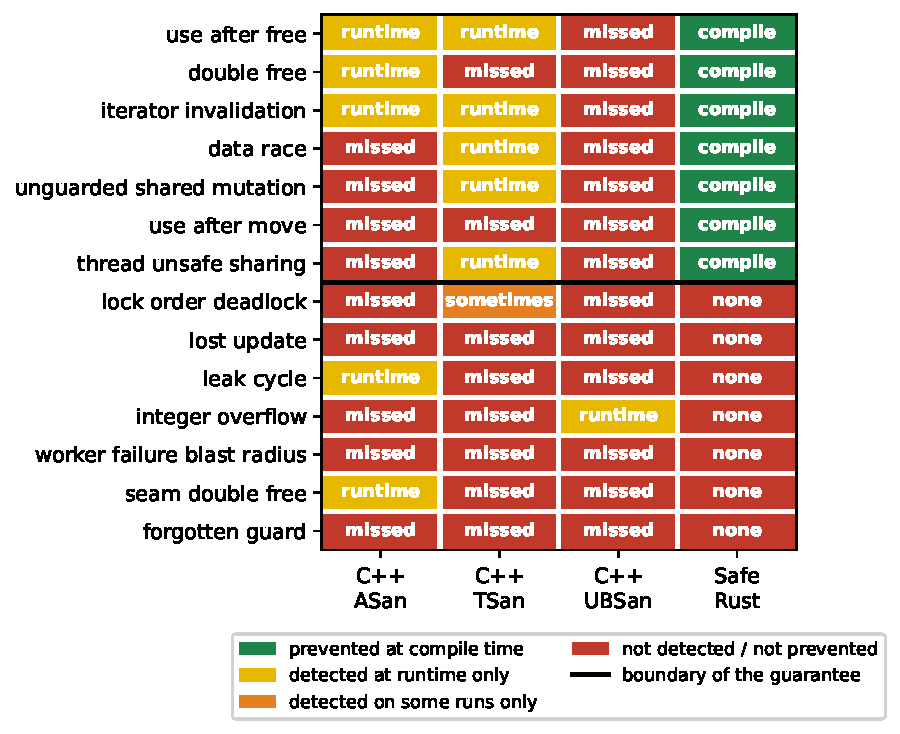
\includegraphics[width=0.72\linewidth]{figures/fig_taxonomy.pdf}
\caption[Where the guarantee stops: the outcome matrix]{The outcomes of Table~\ref{tab:taxonomy} drawn as a matrix, generated from the same
taxonomy log (Section~\ref{sec:repro}). Above the rule the Rust column is a single colour: every
defect is a compile error, so none can be written. The C++ columns there are a patchwork instead,
and no one sanitiser covers them. The use-after-move row is the one no sanitiser covers at all.
Below the rule the Rust column joins them, and on the
reference-cycle leak and the release-build overflow the C++ tooling is ahead. The lock-order
deadlock is the one cell where a tool reports intermittently: ThreadSanitizer flags the inversion
in $\DeadlockTsanHits$ of $\DeadlockTsanRuns$ runs while the program deadlocks on every
one.\label{fig:taxonomy}}
\end{figure}

\subsection{Migration (RQ4)}\label{sec:migrationresults}
Incremental adoption is assessed with a working prototype, built in the direction a real
migration takes: an existing C++ host keeps a Rust component behind a C ABI. The Rust
service is exposed through a thin \texttt{extern "C"} seam in a \emph{separate} crate that
depends on the unmodified core library, so adopting the component needs no change to the
component itself. The C++ host sees only an opaque handle and a set of plain-C entry points
(a hand-written header, no generated bindings), and it drives the full UE lifecycle across the
boundary. The error model crosses intact, so a duplicate connection
setup returns \texttt{InvalidState} through the seam. Figure~\ref{fig:ffiseam} shows the
resulting structure and where the \texttt{unsafe} sits.

\begin{figure}[ht]
\centering
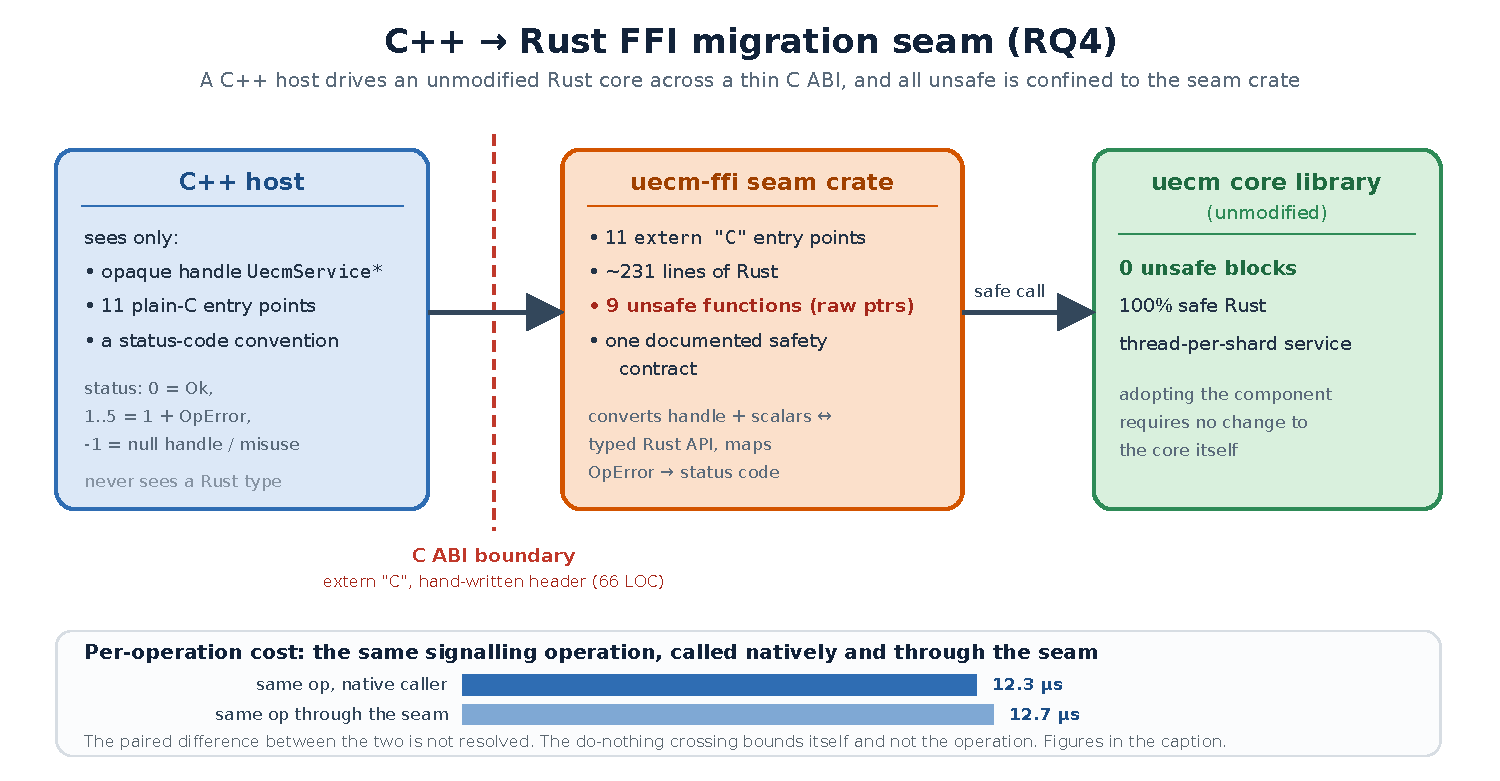
\includegraphics[width=0.78\linewidth]{diagrams/pdf/07_ffi_seam.pdf}
\caption[The C++-to-Rust FFI migration seam]{The C++-to-Rust FFI migration seam. The C++ host sees only an opaque handle, $\FfiEntryPoints$
plain-C entry points, and a status-code convention. A thin \texttt{extern "C"} seam crate
concentrates all of the raw-pointer \texttt{unsafe} ($\FfiUnsafeFns$ functions) and calls the unmodified Rust
core, which remains free of \texttt{unsafe}. The band along the bottom is the comparison the
argument rests on: the same signalling operation called natively at $\FfiOpNative$~\textmu s and
through the seam at $\FfiOpSeam$~\textmu s, whose paired difference is not resolved and is bounded
at $\FfiOpBoundPct\%$ of one operation. The two bars are meant to look alike. The do-nothing
crossing costs $\FfiCrossing$~ns and bounds only itself.\label{fig:ffiseam}}
\end{figure}

Table~\ref{tab:ffi} summarises the interop cost. The
seam is small: $\FfiEntryPoints$ C-ABI entry points in $\FfiSeamLines$ lines of Rust, plus a
$\FfiHeaderLines$-line C
header, with no third-party FFI dependency. The safety boundary is clean, since the core library
stays free of \texttt{unsafe} and the raw-pointer handling the C ABI requires is confined
to the seam crate, in its $\FfiUnsafeFns$ \texttt{unsafe} functions, under a single documented
safety contract. The C++ side never sees a Rust type.

\begin{table}[H]
\centering
\caption[FFI migration prototype: seam size, safety, and cost]{FFI migration prototype: seam size, safety boundary, and per-call interop cost
(C++ host calling the Rust component across a C ABI, \texttt{-O2}). The core library is
unmodified and \texttt{unsafe}-free. All interop is confined to the seam crate. The last
three rows are the direct comparison: one signalling operation on the same service
configuration and the same loop, invoked natively and then through the seam, so the
difference isolates what the boundary adds rather than what the operation
costs.\label{tab:ffi}}
\begin{tabular}{l r}
\hline\hline
Metric & Value \\
\hline
C-ABI entry points & 12 \\
Seam size (Rust \texttt{lib.rs}) & 231 LOC \\
Hand-written C header & 66 LOC \\
\texttt{unsafe} in core library & 0 \\
\texttt{unsafe} in FFI seam & 12 \\
Raw FFI crossing & 2.54 ns/call \\
Signaling op, native caller & 12.3 \textmu s/call \\
Signaling op, through the seam & 12.7 \textmu s/call \\
Seam cost per operation (paired) & $+192$ ns $[-954, +1341]$ \\
\quad as a fraction of the operation & $+10.91\%$ at the upper bound
\\
\hline
\end{tabular}
\end{table}

The per-call cost is measured twice, and only the second measurement answers RQ4's question. The
first is the crossing itself: a do-nothing \texttt{extern "C"} call costs $\FfiCrossing$~ns, an
ordinary indirect call, negligible next to the microsecond-scale round-trip of a signalling
operation. That bounds the crossing and says nothing about what the seam does to a real operation.
The round-trip is dominated by a cross-thread handoff, and an argument that the handoff ``would be
paid identically anyway'' is reasoning standing in for a measurement.

The measurement is therefore made directly. The same signalling operation, on the same service
configuration and in the same loop, is invoked natively from Rust and then from C++ through the
seam, interleaved over \FfiOpRepeats{} repeats so the pair is matched. The paired difference is
$\FfiOpDelta$~ns per operation, with a bootstrap interval of $[\FfiOpDeltaLo, \FfiOpDeltaHi]$~ns
and an exact paired $p$ of $\FfiOpP$. No cost is detected. More usefully, the interval
bounds any cost the measurement could have missed at $\FfiOpBoundPct\%$ of the operation. The
interleaving is not optional here. A single pass of each, run while preparing this section,
made the seam look \emph{faster} than calling natively by a third, because the run-to-run
spread of the handoff on a shared host is far wider than anything a C ABI could contribute.
Figure~\ref{fig:fficost} shows the repeats behind those numbers, and its left panel is that
spread: the pairs cross, over a range an order of magnitude wider than the difference under test.

\begin{figure}[ht]
\centering
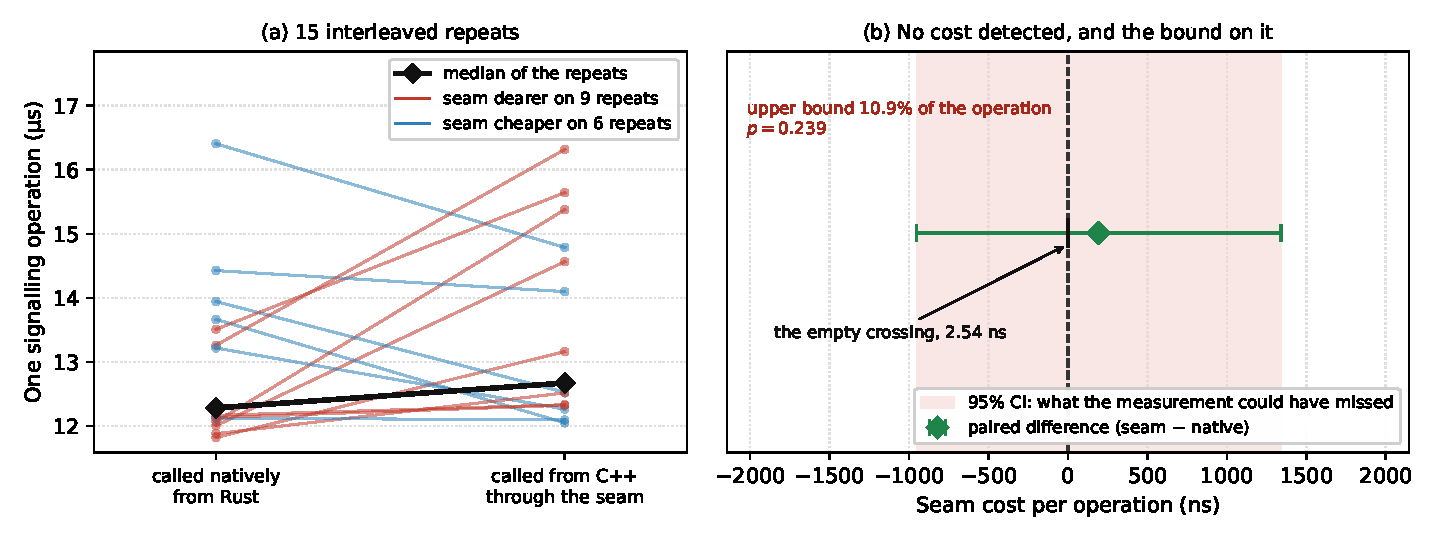
\includegraphics[width=0.78\linewidth]{figures/fig_ffi_cost.pdf}
\caption[The seam's cost on one operation, against its own uncertainty]{The interoperability cost measured on a real operation rather than inferred from an empty
call. \textbf{(a)} The same signalling operation invoked natively from Rust and from C++ through
the seam, one line per interleaved repeat, with the medians in black. \textbf{(b)} The pairs
reduced to their difference: $\FfiOpDelta$~ns per operation with a bootstrap $95\%$ interval of
$[\FfiOpDeltaLo, \FfiOpDeltaHi]$~ns and an exact paired $p$ of $\FfiOpP$. No cost is detected, and
the upper end of that interval is what bounds the cost the measurement could have missed at
$\FfiOpBoundPct\%$ of the operation. The empty \texttt{extern "C"} crossing, $\FfiCrossing$~ns, is
marked for scale rather than as the answer: it is indistinguishable from zero on the axis the
operation is measured on.\label{fig:fficost}}
\end{figure}

The main engineering effort therefore goes into \emph{designing} a C-compatible API
surface, with an opaque handle, scalar-typed operations and a status convention, and not into
runtime overhead. The reverse direction (Rust calling into C++) is symmetric, but it needs
a C-ABI wrapper on the C++ side and it brings \texttt{unsafe} back to the Rust caller. The
prototype and its measurements inform the migration guidelines of
Chapter~\ref{chapter:discussion}.

\paragraph{Three cost axes the seam does not reach.}
RQ4 asks what incremental adoption costs in effort, interoperability and risk. The seam answers
the middle term with a measurement, and it leaves the other two to its own line counts, which
describe one component and say nothing about the work of building it. Three further axes are
measured here, chosen because a team asks each of them before any of the questions answered so
far: how long the toolchain takes, how large the artefact is, and how much code of unknown origin
a configuration pulls in. Table~\ref{tab:adoption} collects them.

\begin{table}[tp]
\centering
\small
\caption[Adoption-cost axes: build time, static footprint, third-party surface]{Adoption-cost
axes beyond the seam. Build time is the median of \AdoptRepeats{} interleaved repeats at
\AdoptJobs{} parallel jobs on the local development machine (\texttt{g++~13.3},
\texttt{rustc~1.97}), warm-up repeats discarded. ``First-party only'' rebuilds the same Rust
targets with the dependency tree left warm, so the difference above it is what the ecosystem
costs and not what the compiler does. Footprint is the \texttt{\FootTarget} binary, the tightest
matched executable pair in the study, reported at each toolchain's default linkage and then at
both matched policies, because the defaults differ and the ordering depends on which policy is
held. Crate counts are transitive and come from \texttt{Cargo.lock}. The \texttt{unsafe} cell is
empty for C++ because the language marks no such region, so no count exists to
compare.\label{tab:adoption}}
\begin{tabular}{@{}l r r@{}}
\hline\hline
Measure & C++ & Rust \\
\hline
\gentablebody{figures/tab_adoption.tex}\\
\hline
\end{tabular}
\end{table}

Binary sizes and dependency counts are environment-insensitive in the sense
Section~\ref{sec:safetyresults} gives the defect catalogue, so they carry from this measurement
unchanged. Build time is not, and it is treated accordingly. It was taken on the local development
machine over \AdoptRepeats{} interleaved repeats at \AdoptJobs{} parallel jobs, with the first
repeats discarded so that a cold page cache is not read as a property of a compiler. The absolute
seconds describe that machine. What travels is the paired ratio between two toolchains measured
alternately on one host, which is the same reason the campaign interleaves its variants.

\paragraph{Compile time separates the compiler from the ecosystem.}
On the matched scope, the core library alone with no third-party code on either side,
\BuildLibWallFaster{} finishes sooner and \BuildLibCpuCheaper{} spends less machine time:
$\BuildLibCppWall$~s against $\BuildLibRustWall$~s of wall clock, and $\BuildLibCppCpu$~s against
$\BuildLibRustCpu$~s of CPU. The orderings disagree because they measure different things, and
the wall clock is the weaker. The C++ library is two translation units, so at
\AdoptJobs{} available jobs only two can ever run, while \texttt{rustc} splits its one crate into
codegen units and kept about three cores busy. Wall clock at this scope rewards the
file layout of this codebase as much as either toolchain, and CPU time is the comparison that
does not.

The full build is where the practical objection to Rust adoption usually lands, and at first
reading it holds. Every default target costs $\BuildAllRustCpu$~s of CPU against
$\BuildAllCppCpu$~s, a factor of $\BuildAllCpuRatio$. Breaking that figure apart moves it somewhere
more useful. Rebuilt with the dependency tree left warm, the same Rust targets cost
$\BuildAllFirstPartyCpu$~s. So $\BuildDepShareCpu\%$ of the clean build is third-party code, and
the project's own code compiles in $\BuildAllFirstPartyCpuRatio$ times the CPU \texttt{g++} needs
for its equivalent. On this codebase the compiler is not what makes the build slow. Two
qualifications bound that reading: the two target sets are close and not identical, and the C++
dependencies are not absent but precompiled into the distribution as shared libraries, which
is a real benefit of a mature ecosystem and not an artefact of the accounting.

\paragraph{The incremental loop is quicker in C++ and less predictable.}
After one edit to an implementation file, C++ rebuilds in $\BuildIncCppTu$~s, which is
$\BuildIncTuRatio$ times quicker than Rust's $\BuildIncRust$~s. After one edit to a core header it
takes $\BuildIncCppHeader$~s. That is $\BuildIncHeaderRatio$ times slower than Rust and, measured
in CPU, indistinguishable from building the tree from scratch. The Rust figure does not move.
Touching every file in the crate costs $\BuildAllFirstPartyWall$~s against $\BuildIncRust$~s for
touching one, because the unit of compilation is the crate and not the file. So the edit-compile
loop is faster in C++ where an edit stays inside a translation unit and slower where it does not,
and which case dominates a working day depends on a codebase's header discipline rather than on
either language. The shape will be familiar from RQ1: the C++ figure is the better
one at the median and the worse one in the tail.

\paragraph{The footprint ordering reverses with the linkage policy.}
Built as each toolchain ships by default, the Rust \texttt{\FootTarget} binary is
$\FootShippedRatio$ times the size of the C++ one, $\FootRustShipped$~KiB against
$\FootCppShipped$. That comparison is between two linkage policies and not between two languages,
because \texttt{g++} leaves \texttt{libstdc++} to the dynamic loader while \texttt{rustc} links its
standard library into the binary. Measured at a matched policy the gap narrows and then changes
sign. With both standard libraries resolved dynamically, \FootDynamicSmaller{} is smaller by
$\FootDynamicRatio$ times. With both linked statically, \FootStaticSmaller{} is smaller by
$\FootStaticRatioAbs$ times.

The reversal has a measured cause and not an argued one. $\FootCppLocaleShare\%$ of the sized
symbols in the statically linked C++ binary are locale and stream facets, among them the money,
date and wide-character facets this program never instantiates, because a static
\texttt{libstdc++} link brings the facet table in as one set. Neither dynamic configuration is
free either, because each leaves a library on the host to be paid for once: $\FootSharedCpp$~KiB
for \texttt{libstdc++} against $\FootSharedRust$~KiB for Rust's shared standard library. The
conclusion worth carrying is that the question has three answers, and the $\FootShippedRatio\times$
figure is the least informative of them. For a self-contained artefact, which is what a container
image or an appliance wants, the ordering favours \FootStaticSmaller{}.

\paragraph{The compared component resolves no third-party code at all.}
The standard objection to Rust in a regulated codebase is transitive-dependency risk, and on the
artefact this study compares it does not arise: $\DepsCore$ crates and $\CoreUnsafe$
\texttt{unsafe} sites, which turns the dependency-free claim of Section~\ref{sec:idioms} into a
measurement rather than an assertion. A surface appears in the configurations around that
component. Linking the matched allocator resolves $\DepsJemalloc$ crates, of which
$\DepsJemallocShipping$ reach the artefact and $\DepsJemallocBuildOnly$ only run while it is being
built. That distinction matters, because a build dependency puts no instruction in the
binary and still runs code on the build machine. The benchmark harness resolves $\DepsHarness$,
and counted with one syntactic rule those two trees hold
$\DepsUnsafeJemalloc$ and $\DepsUnsafeHarness$ \texttt{unsafe} sites.

Two readings should be kept apart. The count bounds where an audit would have to look and is not
a risk score, since a crate concentrating its \texttt{unsafe} in one large block scores below one
that spreads the same work across many small ones. The C++ column is empty by construction and
not by advantage: the language marks no such region, so the whole program stands where
Rust's \texttt{unsafe} blocks stand and a zero would be a category error. The axis
establishes that the component which would ship carries none of this project's unaudited code,
and that the largest surface belongs to the measurement apparatus.

\chapter{Discussion\label{chapter:discussion}}

\section{Summary of findings}
Table~\ref{tab:findings} collects the headline finding for each research question, together with the
strength of the current evidence. The safety results (RQ2) do not depend on the measurement
environment at all. The migration results (RQ4) depend on it along one axis only, because build
time is a timing measurement, which is why it is reported as a paired ratio. The performance and
resource results do depend on the environment, and the honest division now falls inside RQ1 and not
between chapters. The saturation knee, the overload comparison, and the
resource comparisons are resolved on the host of Section~\ref{sec:testbed}, and they replicate
across the allocator control. So is the far tail below saturation, in Rust's favour, which was the
standing open question of this study for as long as it measured on a virtualised machine. The
division that remains is not between results but between hosts: the same design on the earlier host
could not resolve that percentile at all, and Section~\ref{sec:hostcompare} reports what changed
and what did not.

\begin{table}[tp]
\centering
\caption[Summary of findings per research question]{Summary of findings per research question and the current strength of evidence.
\label{tab:findings}}
\renewcommand{\arraystretch}{1.25}
\begin{tabular}{@{}p{0.06\linewidth} p{0.62\linewidth} p{0.22\linewidth}@{}}
\hline\hline
RQ & Headline finding & Evidence status \\
\hline
RQ1 & The answer divides at saturation. Below it the variants agree to $\PFiftyRange\,\mu$s
($\PFiftySpread\%$) at the median, and the far tail resolves in \FarTailLower{}'s favour, with the
pooled p99.99 of the two \FarTailLower{} variants below both of the others by up to
$\FarTailRange\,\mu$s. The end-to-end number is
only $\BudgetCoreShareMax\%$ operation, so it cannot bound a language effect in any case, while
the operation measured apart is $\BudgetCoreRatio\times$ faster in \BudgetCoreFaster. Past
saturation they diverge decisively, and in both directions: the Rust arms hold their offered rate
one rung further, to $\TrackingLoadRust$~kops/s against $\TrackingLoadCpp$, while at
$\OverloadLoad$~kops/s, where all four have collapsed,
\OverloadSustainedFaster{} sustains $\OverloadThrRatio\times$ the throughput of
\OverloadSustainedSlower{} in \OverloadThrAgree{} repeats under both allocators. & Overload,
operation and far tail: resolved, and each reproduced at a second shard count.
Mechanism: tested. Primitives alone insufficient. The saturation-limit gap is descriptive, not
tested \\
RQ2 & All seven injected memory-safety and data-race classes are prevented at compile time in
safe Rust, where in C++ each compiles and is caught, if at all, only at runtime and by no single
sanitiser. The guarantee stops there: the seven boundary classes compile in both languages, and
on the leak and the release-build overflow the C++ tooling reports what Rust's does not. &
Final \\
RQ3 & A memory penalty that reproduces: $\RssLangDiffLo$--$\RssLangDiffHi$~MiB more peak RSS in
the Rust build under \emph{both} allocators, and the same size on all three machines measured. The
allocator's own $\RssAllocDiffLo$--$\RssAllocDiffHi$~MiB is comparable here and was an order of
magnitude larger on the virtualised host, so their ratio does not travel
(Section~\ref{sec:hostcompare}). CPU inverts across the regimes: Rust draws up to
$\CpuDiffAbsMax$ percentage points less below saturation and $\OverloadCpuPerOpRatio\times$ more
per completed operation above it. & Memory: resolved, and located outside the allocator by its own
accounting. CPU: resolved in both regimes, opposite signs, and resolved with one sign on bare metal
below saturation \\
RQ4 & The seam is small and keeps the core \texttt{unsafe}-free at compile time. Measured against
the same operation called natively, no cost is detected and any tax is bounded at
$\FfiOpBoundPct\%$ of an operation. The real cost is API design. The core remains exposed at run
time to memory errors in the C++ host it shares an address space with. On the adoption axes beyond
the seam, $\BuildDepShareCpu\%$ of the Rust clean build is third-party code and the project's own
code compiles in $\BuildAllFirstPartyCpuRatio$ times the CPU \texttt{g++} needs, the footprint
ordering reverses with the linkage policy, and the compared component resolves $\DepsCore$ crates.
& Final. Build-time absolutes are host-bound, the ratio is not \\
\hline
\end{tabular}
\end{table}

\section{Discussion on the research questions}\label{sec:rqdiscussion}
\paragraph{RQ1 (predictability).} RQ1 has two halves, below saturation and beyond it, and the
campaign answers them differently enough that reporting either alone would misrepresent the
result.

Below saturation the languages are equivalent in central behaviour, by a margin no deployment
would notice. The small paired difference at the median that does clear the correction is a
fraction of a $\PFiftyMedian\,\mu$s operation. The far tail in this regime is a different matter,
and one a deployment would also care about. There the result is an ordering rather than a null, and
it favours \FarTailLower{}: pooled over millions of operations per variant, the two languages'
p99.99 values do not meet, and the gap between the extremes is $\FarTailRange\,\mu$s, roughly the
width of a whole median operation. So the equivalence claimed at the median does not extend up the
distribution, and the direction in which it fails is the one that favours the safer language. That
is a difference in the percentile a deployment sizes its margin from, and it is reproduced at a
second shard count on a second machine (Section~\ref{sec:hostcompare}), which is as much
corroboration as this study can offer for any timing result. The central result is consistent with
the wider evidence that
Rust's safety checks are largely absorbed by modern out-of-order
CPUs~\cite{balasubramanian2017rust,emmerich2019drivers}. It is also weaker than it
looks, for the reason Section~\ref{sec:budget} gives. The operation the
languages execute is $\BudgetCoreShareMax\%$ of what the sweep measures. An end-to-end null in
a design dominated by a cross-thread wakeup therefore says something about the design and not
about the languages. Measured on its own, the operation differs by $\BudgetCoreRatio\times$.

Beyond saturation the answer changes in kind, and it changes twice. Where each implementation stops
meeting its offered rate differs by one rung of the ladder, with the Rust arms holding to
$\TrackingLoadRust$~kops/s against the C++ arms' $\TrackingLoadCpp$. Deeper still, once both have
collapsed, the ordering reverses: the C++ build sustains $\OverloadThrRatio$ times the throughput of
the Rust one while drawing more CPU per completed operation, reproducibly and at the corrected floor
of the whole test family (Section~\ref{sec:overload}). Only the second of those is tested, and
Section~\ref{sec:perfresults} says why the first is not. So the practical form of RQ1's answer is
not that the language choice is irrelevant to predictability. It is irrelevant \emph{until the
service stops coping}, and around that point it decides both when coping stops and how
much work still gets done afterwards. A comparison that stopped at nominal load, as most in this
literature do, would have concluded the opposite with the same apparatus.

That the two effects point in opposite directions is not a contradiction to be resolved but the
reason a single verdict on this question would be false. A service sized to run below its knee
should prefer the arm with the higher knee. A service that will be driven past every arm's knee by a
signalling storm should prefer the one that degrades less steeply. Those are different deployment
questions, and this study answers them differently.

That reframes the closest prior work instead of merely agreeing with it. Arvidsson and Kaller
measure this quantity for 5G control-plane procedures and find Rust's 99th percentile degrading
faster beyond a threshold request rate. They trace it to stackless
\texttt{async}/\texttt{await}, which permits a context switch immediately before an I/O operation
begins~\cite{arvidsson2025async}. Section~\ref{sec:relatedwork} accepts that attribution, and
this study was built to exclude the confound behind it: one worker per shard over a bounded
blocking queue, and no asynchronous runtime on either side.

Section~\ref{sec:rqs}
committed in advance to what each outcome would mean, and the second branch is the one that
fired. A degradation past a threshold rate appeared with the concurrency model held fixed, so the
asynchronous runtime cannot be the only place such an effect starts. The prediction also
named where to look first if that happened: bounds and overflow
checking~\cite{zhang2022runtime,harris2023morello}. That part of it was wrong. The effect
appears only once the handoff path is contended, which points instead at the two standard
libraries' blocking primitives recorded in Table~\ref{tab:idioms}. Section~\ref{sec:contention}
then tests whether those primitives alone explain the gap, and they do not reproduce the
full-service ordering at significance. That narrows the cause to extra work on the C++ handoff
path and not to the safety model. Recording that the prediction resolved against its own first
hypothesis, and that the follow-up microbenchmark refined the attribution instead of confirming it,
is more useful to the next study than quietly swapping in the explanation that survived.

\paragraph{RQ2 (safety).} The result does not depend on the environment. What makes it
interesting is not the half that confirms the expectation, but the half that bounds it. Within
its scope the guarantee is absolute in one specific sense, and the difference from C++ is one of
kind and not of degree. A compiler that refuses to build a program rules the defect out of
every execution. A sanitiser rules it out only of the executions an instrumented test
happens to take. What is absolute is the execution coverage, not the breadth of the catalogue.
The scope itself is still the $\FaultClasses$ programs written for it.
That fits the CVE evidence that Rust memory-safety bugs always involve
\texttt{unsafe}~\cite{xu2021rustcve}, and the caution that unsafety can still spread
through dependencies~\cite{evans2020rust}, which is why keeping the core \texttt{unsafe}-free
matters. The seam double-free is that evidence reproduced under controlled conditions: the one
class in this catalogue that safe Rust rejects and unsafe Rust does not.

The one case that reaches past the written programs is the lifecycle defect of
Section~\ref{sec:safetyresults}. It was found in the implementation, not written for
the catalogue, and it revises the picture in two directions at once. It strengthens the cost
argument. A real defect in code written to be correct survived the entire verification
apparatus of this study, meaning tests, parity vectors, and three sanitisers, purely because
nothing exercised the path. Runtime detection that depends on test coverage is a weaker
proposition in practice than it looks in a table where every row is driven deliberately.

It also
narrows what may be credited to Rust, because the contribution there was a bounds check and not
a proof. The honest generalisation is that
the guarantee worth budgeting for is \emph{checked by default} and not \emph{ruled out at
compile time}. The root cause is worth naming too, because it is a risk of the method
and not of either language. A specification that states a prohibition without assigning a
mechanism leaves each implementation to fail in its own idiom. The two idioms here are a
panic and a use-after-free.

Where the guarantee stops matters just as much to a vendor deciding what Rust buys, and the two
boundary classes are instructive for different reasons. The lock-order deadlock shows that Rust
reasons about \emph{aliasing} and not about \emph{acquisition order}. A \texttt{Mutex} guard is an
ordinary value whose lifetime the borrow checker tracks perfectly, and tracking it perfectly
says nothing about whether two threads take their locks in compatible orders. The tooling built
around the language confirms that this is a boundary and not an artefact of the injected example.
Static deadlock detection for Rust is an active research problem
in its own right~\cite{zhang2026deadlock}, and model checkers for Rust kernel code are motivated
explicitly by the observation that ownership and borrowing leave data races, deadlocks, and
livelocks reachable~\cite{tang2025converos}.

The lost update is sharper still. It escapes
ThreadSanitizer for precisely the reason it escapes the borrow checker, as
Section~\ref{sec:safetyresults} sets out. With every access correctly synchronised there is no
unsynchronised access to find. Nor is the class marginal. In a field study of $105$ real
concurrency bugs, about a third of the non-deadlock cases violated the order the programmers
intended, not their locking, and the authors record that such intentions are not readily
expressible through locks at all~\cite{lu2008mistakes}. The distinction
it exposes, between a data race and a race
condition, is the one the phrase ``thread safety'' routinely runs together, and Rust removes only
the first.

The practical consequence is that adopting Rust retires one category of concurrency defect
completely while leaving another untouched. The category left untouched is the one that fails
silently, corrupting a counter or a state decision instead of crashing. A migration plan that
treats ``memory-safe'' as ``concurrency-safe'' would therefore mis-budget its review and testing
effort. That is why this boundary is reported as a first-class result and not as a caveat.
Figure~\ref{fig:boundary} draws the boundary itself, with the two halves of the
guarantee on either side of the line and the mechanism that does the enforcing, or the absence
of one, named in each panel. It carries the two concurrency cases rather than all seven outside
the guarantee, because they are the pair that makes the distinction, and
Table~\ref{tab:taxonomy} holds the full catalogue.

\begin{figure}[ht]
\centering
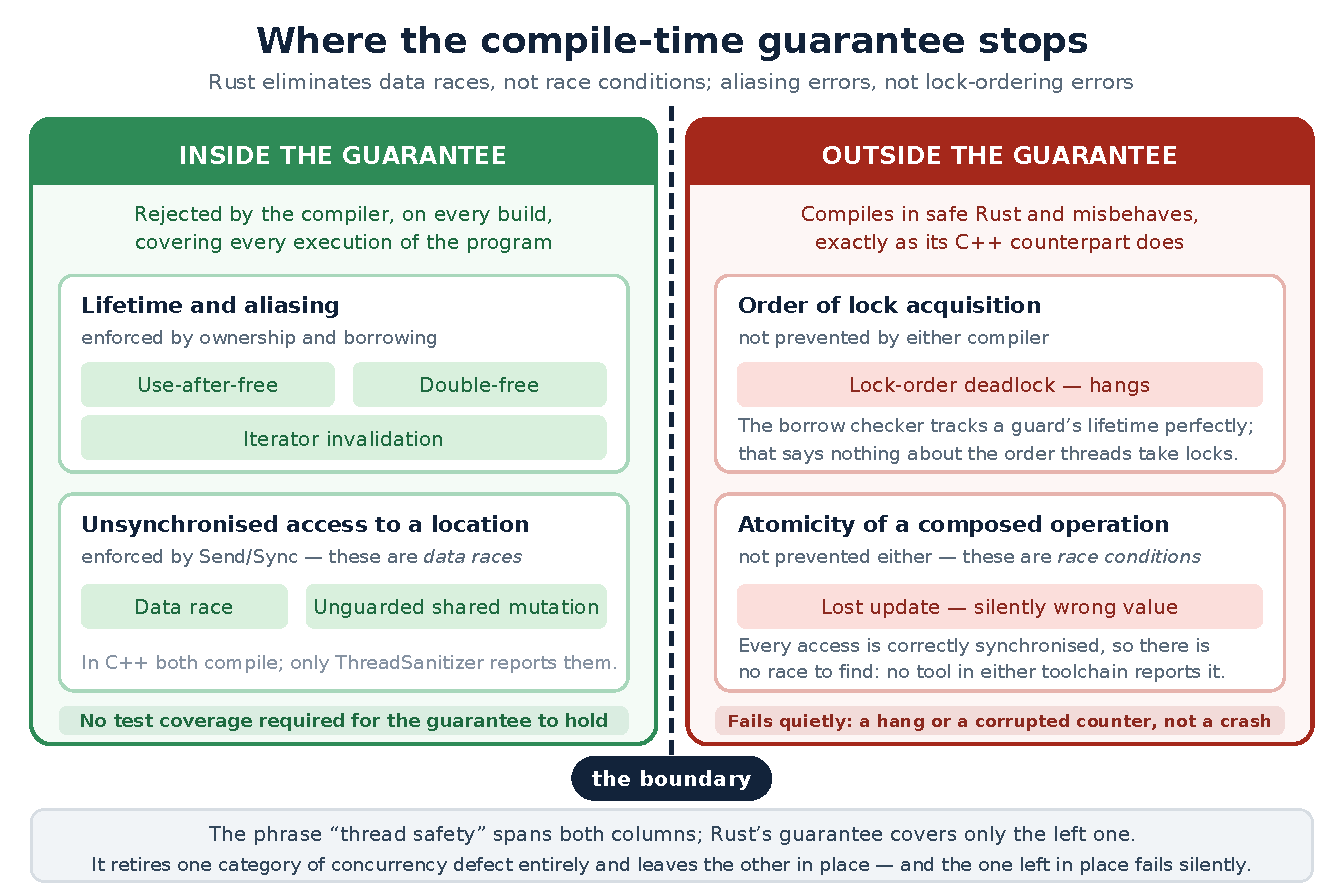
\includegraphics[width=0.78\linewidth]{diagrams/pdf/17_guarantee_boundary.pdf}
\caption[Where Rust's compile-time guarantee stops]{Where the compile-time guarantee stops. On the left are the classes safe Rust rejects
outright, grouped by the \emph{mechanism} that rejects them rather than by defect
family: ownership and borrowing for lifetime and aliasing errors,
which is why iterator invalidation sits with them, and the \texttt{Send}/\texttt{Sync}
discipline for unsynchronised access to a location. On the right are the classes the
catalogue included to find the edge, which neither compiler prevents. The diagram names one
class per mechanism and is not the catalogue, which
Table~\ref{tab:defectmap} lists in full: the use-after-move belongs with the
ownership cases on the left and the shared thread-unsafe handle with the \texttt{Send}/\texttt{Sync}
ones, while the leak, the release-build overflow, the worker-failure case, the seam double-free
and the forgotten guard sit alongside the two on the right. The phrase ``thread safety'' spans
both sides of the line, and the guarantee covers only the left. The line itself moves once more
than the diagram can show, because a program that writes \texttt{unsafe} crosses it
voluntarily.\label{fig:boundary}}
\end{figure}

\paragraph{RQ3 (overhead).} The answer splits by resource, and the splits do not all point the
same way. On memory there is a penalty. The Rust build carries a few MiB more peak resident set
than the C++ build, and it keeps that sign under both allocators. Two things make it credible
beyond the $p$-value. Peak RSS is a run-level maximum and not a
tail statistic, so the scheduling jitter that destroys the p99 does not touch it. And it reproduces
on a second machine with a different compiler (Section~\ref{sec:baremetal}), which no other
timing-adjacent result in this study can claim. The useful way to size it is against the allocator's
own effect, and that comparison is the part which does \emph{not} travel. The two are of comparable
size on the reported host and on the second bare-metal one, while on the virtualised host the
allocator's was an order of magnitude larger, because the allocator effect shrank by more than ten
times across the change of machine and the language effect did not move. So the language effect
replicates and its ratio to the allocator's does not. A team choosing between these two languages
moves a few MiB either way, and whether that is more or less than choosing between these two
allocators is a question about the machine.

On CPU the answer depends on the load, and that dependence is the finding rather than a
complication. Below saturation Rust draws slightly \emph{less}, consistently under both
allocators. Past saturation the sign flips and the magnitude grows
(Section~\ref{sec:overload}). A single number for ``the CPU cost of
Rust's safety model'' would therefore average two regimes that behave in opposite directions, and
neither figure is the safety model in any case. Throughput splits the same way and for the same
reason. Below saturation there is nothing to measure, because achieved throughput tracks offered
load by construction. Above it sits the largest effect in the study.

Back to the memory penalty, because three things bound what it licenses and the third is new. It is
a fixed cost rather than a per-context one, so
its share of a deployment's footprint falls as the deployment grows. It is also located, and that
took an instrument no virtualised host in this study offered: the allocator's own accounting puts
the difference \emph{outside} the allocator, since the Rust build holds less live data and fewer
resident bytes inside \texttt{jemalloc} and still peaks $\BmJeRssDelta$~MiB higher
(Section~\ref{sec:hostcompare}). What a Rust process carries before it allocates is the standard
library and the runtime, and that is a one-off charge per process rather than a tax on the work.
And it should not be widened into a claim about Rust's safety
model, because nothing here isolates bounds checking or ownership-driven copying as the cause.
The mechanisms the literature has localised~\cite{zhang2022runtime,harris2023morello}
are candidates to test, not conclusions to import. What can be said is narrower and still
useful to a vendor sizing a control-plane node. Adopting Rust here costs a few megabytes of
fixed footprint per process, and it buys a faster core operation
(Section~\ref{sec:budget}) that this workload's structure never turns into throughput below
saturation, and that turns into a deficit above it.

The sign of that result is worth defending, because one of the closest prior works in the domain
reports the opposite sign, while two others agree with it. Agreement first, since it is quickly
stated. A second Ericsson-hosted study of RAN node management software found Rust's peak memory
usage generally higher than C's~\cite{olsson2023ranmgmt}, and a matched pair of user-space device
drivers outside telecom put the Rust version's footprint about 29\% above the C
version's~\cite{sundvisson2026drivers}. Neither separates the allocator from the language, which
is the distinction Section~\ref{sec:resources} rests on, so they support the direction of the
effect and not the way it splits.

The disagreement is the more instructive case. Karlb\"ack and Or\"o measure peak resident set on a RAN workload and
find Rust the \emph{lowest} of the three languages and C++ the highest, with the gap widening
as concurrency rises. They call the pattern surprising and attribute it tentatively to the initial
stack size of the green threads~\cite{karlback2021ran}. The two
findings are compatible once it is clear that they measure different quantities. Their C++ runs
on Boost.Fibers, which allocates a stack per fiber, so ten thousand concurrent sequences cost
ten thousand stacks. Their Rust runs on Tokio, where a task is a heap-allocated future of a few
hundred bytes. What their figures capture is therefore the per-context cost of the concurrency
runtime, which is exactly why it grows with the number of contexts.

The design measured here
has no green threads on either side. A fixed thread-per-shard pool leaves no per-context
allocation to differ, and what remains is the fixed footprint reported above, constant in the
number of UEs and not proportional to it. Their disagreement with this result is therefore
between two concurrency runtimes and not between two languages, which is as direct a
demonstration as the literature offers of why this study holds the concurrency model fixed. It
also sharpens the caveat attached to the present number. It licenses nothing about Rust's
memory behaviour under a task-per-UE design, which is a different experiment.

\paragraph{RQ4 (migration).} The prototype shows that incremental adoption is technically
cheap. A C++ host can call an unmodified Rust core across a thin C-ABI seam whose cost on a
real operation is bounded at $\FfiOpBoundPct\%$, and all \texttt{unsafe} stays inside the seam.
That bound comes from the matched comparison of Section~\ref{sec:migrationresults}, not
from setting an empty crossing
against a full round-trip. The two are not the same experiment, and on this host a single
unpaired pass of each was enough to flip the apparent ordering. The dominant cost is
therefore human and not machine: designing a C-compatible surface and, as the adoption
studies report~\cite{fulton2021adopting,crichton2024learning}, climbing Rust's learning curve.
That makes migration risk an organisational concern and not a performance one, and the two
largest documented adoptions into existing C and C++ codebases report the same ordering of
costs~\cite{li2026rustlinux,fan2026android}.

One boundary on that result has to be drawn explicitly, because the natural reading overstates
it. ``All \texttt{unsafe} confined to the seam'' is a claim about what the compiler verifies,
and it is true as measured. The core crate contains no \texttt{unsafe}, and every raw-pointer
operation sits in $\FfiUnsafeFns$ reviewable functions. It is not a claim that the core is protected at run
time. Host and component share an address space, and a memory error on the C++ side can corrupt
Rust-owned data however carefully the Rust side was checked. That is why the remedies proposed
in the literature isolate the two heaps with hardware support instead of relying on interface
discipline~\cite{rivera2021galeed,kirth2022pkrusafe}, and the defect classes that arise at such
boundaries have been catalogued in their own right~\cite{li2022crosslang}. So a migration
of this shape buys less than ``the Rust part is safe''. It buys a migrated
component that stops \emph{contributing} new memory-safety defects, while it stays exposed to those
of the host until the host is migrated too. That is still the right direction of travel, and it
is a reason to sequence a migration so that the components sharing the most mutable state cross
over together instead of one at a time.

The three axes measured beyond the seam sharpen the same conclusion, and they complicate two of its
folk versions. Build time is the objection most often raised against Rust in a large codebase, and
it survives only in the aggregate. The full build does cost $\BuildAllCpuRatio$ times the CPU. But
$\BuildDepShareCpu\%$ of that is third-party code, so the project's own source compiles for
$\BuildAllFirstPartyCpuRatio$ times what \texttt{g++} spends on its equivalent. An organisation
worried about build time should look at its dependency budget before it looks at the
compiler. The edit-compile loop is the axis where C++ genuinely leads, and it leads unevenly. Its
advantage holds for edits inside a translation unit and reverses for edits to a widely included
header.

Binary size behaves worse than an argument would predict. The $\FootShippedRatio\times$
figure that gets quoted compares two linkage policies, and once the policy is held fixed
the ordering depends on which one was chosen. The axis that matters most for a regulated codebase
has the cleanest answer of the three. The component compared here resolves no third-party code
and contains no \texttt{unsafe}, so the transitive-dependency argument against Rust adoption does
not reach the artefact under discussion.

\section{Revisiting the hypotheses}\label{sec:hypotheses}
Section~\ref{sec:rqs} committed to three hypotheses before any measurement was
taken. Stating their disposition explicitly, rather than letting the results speak for
themselves, is what distinguishes a test from a description.

\begin{description}
  \item[H1: supported below saturation, refuted above it.]
        The hypothesis had two parts: that the languages are performance-equivalent below
        saturation, and that any difference is confined to the far tail. The first is
        supported. The second is refuted, and not in the direction the wording anticipated,
        for the reasons Section~\ref{sec:rqdiscussion} gives. The largest difference the study
        found lies in overload, which H1 did not consider at all. The hypothesis as written would
        have led the campaign to look in the wrong place, and the result was found only because the
        sweep was pushed past saturation on methodological grounds rather than in expectation of it.

        The clause H1 did name turns out to be half right, and the half it gets right was the
        harder one to reach. For most of this study the far tail could not be resolved at all, so
        on the evidence then available H1's second part was untestable rather than refuted. It is
        resolved now, on the reported campaign, and a difference is present in the far tail below
        saturation in Rust's favour at loads where the median difference is about a microsecond on
        an operation of $\PFiftyMedian\,\mu$s. A second bare-metal campaign at another shard
        count agrees on the direction (Section~\ref{sec:hostcompare}). So H1 was right that the
        far tail is where a below-saturation difference would show up, and wrong that the far tail
        is the only place any difference shows up.

        A second disposition is that the hypothesis is not well posed.
        ``Performance-equivalent'' was written as though it named one quantity.
        Section~\ref{sec:budget} shows it names at least three. There is the delivered operation
        below saturation, where the languages are equivalent. There is the code the compilers
        emit, where they are not, and where the end-to-end measurement dilutes the difference by
        more than two orders of magnitude. And there is sustained work under overload, where they
        are not equivalent either and the difference runs the other way. All three are true, and a
        hypothesis that cannot tell them apart is one this study should have stated more carefully
        before measuring.
  \item[H2: supported in its precise form, refuted in its loose one.] The hypothesis was
        that safe Rust prevents at compile time ``the memory-safety and concurrency defect
        classes that C++ leaves to best-effort detection''. For the seven injected classes of
        that kind it holds without exception. The fault-injection study still refutes
        the broader reading the wording invites. The seven boundary classes are exactly the sort
        C++ leaves to best-effort detection, safe Rust does not prevent them either, and on the
        leak and the release-build overflow the C++ tooling is the one that reports. H2 is
        therefore accepted for memory safety and
        data-race freedom, and rejected for concurrency correctness at large. It also carries an
        unstated precondition, which the seam case makes explicit: the hypothesis is about
        \emph{safe} Rust, and the same class it rules out returns as soon as a program writes
        \texttt{unsafe}. The second reading
        is the one practitioners tend to assume.
  \item[H3: supported, and tested the right way on the second attempt.] The hypothesis was
        that interoperability cost is negligible against the operations invoked. Measured
        directly (Section~\ref{sec:migrationresults}), no cost is detected and any per-operation
        tax is bounded at $\FfiOpBoundPct\%$. What supports the hypothesis is the bound, not the
        failure to detect a difference. The first version of this measurement did
        not deliver that. It set an empty crossing against a full round-trip and inferred the
        answer, which compares two different experiments and would have given
        the right conclusion for the wrong reason. The accompanying claim, that the real cost
        is engineering effort, is supported structurally and not statistically. The seam is
        small and mechanical, but designing its C-compatible surface was the part of the
        prototype that took actual design decisions.
\end{description}

\section{Engineering guidelines for incremental adoption}
\label{sec:guidelines}
The results are meant to be usable, and a vendor weighing Rust for a control-plane component
needs more than a set of measurements. The following guidelines are the practical form of the
evidence above. Each is tied to the finding that supports it, and the limits of that
support are stated and not glossed. A guideline quoted without its limit is how the
RQ2 result becomes ``the migrated component is safe'' and the RQ4 result becomes ``migration is
cheap'', and this study establishes neither. They are given in the order a first migration
would run them.

\paragraph{Choose the first component for its interface, not its size.}
The boundary's run-time cost is bounded at $\FfiOpBoundPct\%$ of an operation (RQ4), so the
criterion for a first Rust component is not how small or how hot it is. It is how narrow and how
scalar its interface is. The seam here stayed at $\FfiEntryPoints$ entry points because the subsystem's API
was already lifecycle-oriented, typed, and free of shared mutable structures crossing the
boundary. A component whose interface passes rich C++ objects, templates, or callbacks will need
those designed out first, and that redesign is the schedule risk, not the FFI.

\paragraph{Put the ABI in its own crate and keep the core \texttt{unsafe}-free.}
Concentrating every raw-pointer operation in a separate seam crate that depends on an unmodified
core (Section~\ref{sec:migrationresults}) is worth adopting as a rule, not treating as an
accident of this prototype. It keeps the dependency-propagation problem Evans et al.\
describe~\cite{evans2020rust} away from the safety-critical code, and it makes the reviewable
surface of the migration a fixed, countable thing. Two qualifications belong with it. It bounds
what has to be \emph{reviewed}, not what can be \emph{corrupted}. While the host remains C++ the
two share a heap, so a team needing the stronger property has to look at in-process
isolation~\cite{rivera2021galeed,kirth2022pkrusafe} and not at interface discipline alone.
And the generated part of a seam is not above suspicion, because binding generators have their own
defect history~\cite{cai2026interop}. Review it as code instead of trusting it as tooling
output.

\paragraph{Do not re-budget concurrency review effort on the strength of memory safety.}
This follows directly from the boundary cases. Adopting Rust removes use-after-free,
double-free, iterator invalidation, and data races from the defect budget entirely, and those
are the classes that dominate the security statistics~\cite{msrc2019memory,google2022android}.
It removes nothing from the deadlock and atomicity-violation budget. Lock-ordering discipline,
invariants about which locks may be held simultaneously, and review for
composed-but-not-atomic operations remain exactly as necessary as they were in C++, and they
should stay in the code-review checklist and the design-review agenda after migration.

\paragraph{Prefer a shared-nothing structure to a shared-and-locked one, in either language.}
The strongest concurrency result in this study belongs to neither language. The
thread-per-shard design removes locks from the hot path altogether, which is why the boundary
defects had to be built as standalone programs instead of found in the implementations.
Where state can be partitioned by a natural key, as UE state can be partitioned by
\texttt{ue\_id}, partitioning it turns a class of concurrency defects into a structural
impossibility for both languages, and it does so without either compiler's help.

\paragraph{Budget for the learning curve, and measure it.}
The dominant cost identified here is human, which matches what adoption studies
report~\cite{fulton2021adopting}. This thesis cannot quantify that cost, because it is a
single-author study, so the guideline is correspondingly modest. Treat the first component as
a training investment with a deliberately generous schedule, and instrument it, recording
review time and defect density, so the second component can be planned on measured effort
instead of assumed effort.

\paragraph{Measure the component, not the round-trip, and do not generalise either.}
The performance findings carry a methodological warning that travels further than the
numbers do. An end-to-end request/response measurement of a design like this one is
$\BudgetCoreShareMax\%$ language and the rest scheduler (Section~\ref{sec:budget}). Below
saturation it will therefore return ``no difference'' between almost any two competent
implementations, and reading that as evidence about the languages is a mistake this study made
before it measured the components apart. A vendor running its own comparison should budget for
both: the end-to-end measurement, which says what a deployment will feel, and the component
measurement, which says what the language is doing.

\paragraph{Sweep past saturation, because that is where the languages stopped agreeing.}
This is the guideline the study would most like to have followed from the start instead of
arriving at. Every conclusion it drew about performance while the sweep stopped at nominal load
was a null. Each was correct at that operating point and silent about the one where the two
implementations differ by $\OverloadThrRatio\times$ (Section~\ref{sec:overload}). The knee is
not a detail at the edge of the graph. For a control plane it is the region that decides whether
a signalling storm degrades service or ends it, and it is where a bounded, blocking design has
no graceful behaviour left. A comparison that stops while the system is still meeting its
offered load has measured the easy half of the question. Sweeping past the knee costs one
more afternoon of machine time.

Beyond both of these, the reusable artifact is the benchmarking framework and not its current
output. The decision it should inform is ``measure this on your component, and measure it past
the point where your component stops coping'', not ``Rust is fast enough, proceed''.

\section{Related work}\label{sec:relatedwork}
Chapter~\ref{chapter:background} set out the ground this work stands on in four strands, and
restating them would add nothing. Each is reduced here to the position it leaves this thesis in,
after which the studies it has to answer to are treated at length.

The performance strand is settled on the average case. Compiled systems languages sit close on
time and energy~\cite{bugden2022rust,pereira2017energy}, Rust's safety is cheap at run
time~\cite{balasubramanian2017rust,levy2017kernel}, and that holds where timing is tightest, in
embedded hypervisors, production cloud infrastructure, and packet processing within a few percent
of a C reference~\cite{mo2023rustshyper,agache2020firecracker,emmerich2019drivers,xiao2024rpkt}.
Where a cost does appear it has been pinned down: to bounds, overflow and division checks, to that
same check set against hardware-enforced capabilities, and to recurring
anti-patterns~\cite{zhang2022runtime,harris2023morello,cui2025perfbugs}. One like-for-like port
puts the bounds-check share at 34\% of a 46\% geometric-mean overhead, and cautions that code
credited with cheap checks has sometimes declared its hot functions
\texttt{unsafe}~\cite{naylor2026cherisimt}. That caveat does not reach the \texttt{unsafe}-free
core compared here. None of this work reports behaviour past a saturation point, which is the
regime this thesis targets.

The safety strand is settled the same partial way, with machine-checked foundations for the safe
fragment and the aliasing discipline \texttt{unsafe} code has to
respect~\cite{jung2018rustbelt,jung2021safe,jung2020stacked}, confirmation that \texttt{unsafe} is
used sparingly and that memory-safety CVEs always involve
it~\cite{qin2020rust,astrauskas2020unsafe,xu2021rustcve}, auditing that finds defects at scale even
so and unsafety spreading through dependency
chains~\cite{bae2021rudra,zheng2024security,qin2024safety,evans2020rust}, and the reports
motivating the shift set against a long record of memory corruption resisting runtime
mitigation~\cite{msrc2019memory,google2022android,google2024securebydesign,cisa2023memorysafe,oncd2024building,szekeres2013sok}.

The interoperability strand qualifies the adoption argument, and Section~\ref{sec:interop} states
its central limit: confining \texttt{unsafe} to a seam does not protect the Rust side, because
foreign code in the same address space can corrupt Rust-owned data
anyway~\cite{rivera2021galeed,kirth2022pkrusafe}. What that section does not cover is reach. The
seam carries its own defect classes and its own tooling bugs, lighter crossing models exist for
embedded use, aliasing patterns expressible in C but not in safe Rust bound translation in
principle, interoperation is the central open problem in embedded Rust, \texttt{unsafe}
concentrates at exactly these boundaries, and the two largest documented adoptions into existing C
and C++ report the resulting friction
empirically~\cite{li2022crosslang,cai2026interop,schuermann2023encapsulated,emre2023aliasing,sharma2024embedded,mccormack2026unsafe,li2026rustlinux,fan2026android}.
Automating the rewrite is not a solved problem either, since current translators still emit code
whose safety the compiler cannot validate~\cite{hong2025ctorust}. That is why the migration cost
measured here is the cost of a hand-written seam.

The fourth strand is the domain and the method: the tail-latency and microsecond-scale
literature~\cite{dean2013tail,barroso2017microseconds,li2014tales,huang2017predictability},
thread-per-core structuring moving the tail in its own right~\cite{enberg2019threadpercore}, O-RAN
disaggregation~\cite{polese2023oran}, control-plane latency as an active target in the core network
too~\cite{liu2023l25gc,park2025ctrlbench}, adoption evidence pointing at the learning curve rather
than run-time cost~\cite{fulton2021adopting,crichton2024learning,ardito2021verbosity}, and standard
guidance on repeat-based evaluation and fault
injection~\cite{georges2007rigorous,natella2016fault}. Rust has mobile-network precedent in the
datapath~\cite{qazi2017pepc} and, on the control-plane side, an open-source gNB-CU with a separated
CU-CP and CU-UP over E1. That last one bears on the gap rather than on the method. It establishes
that the ASN.1 and SCTP protocol surface is no barrier in principle, but it is an existence proof
and not a comparison, reporting no latency and carrying no C++ counterpart built to the same
specification~\cite{alsoran}.

Four systems studies come closest in method, though not in domain, because they too build the
same component twice and attribute the difference. One compares IPC mechanisms implementing a
single network function in both C++ and Rust~\cite{li2021ipc}. RedLeaf is evaluated against C
baselines built for the purpose~\cite{narayanan2020redleaf}. A manual translation of the STAMP
transactional benchmark suite into Rust is the closest published match to this study's design,
because its workload is concurrent and both versions implement one
specification~\cite{suchert2023stamp}. The fourth measures a Rust UDP tunnelling driver in the
Linux kernel against an equivalent C driver~\cite{gonzalez2023rustudp}. That last one is worth a
second look for its method and not its result. It reports Rust slower by 0.19\% at
$p = 1.5 \times 10^{-15}$, a difference overwhelming in statistical terms and negligible in
operational ones. Keeping those two apart is what the pre-committed interval-versus-$p$ rule of
Section~\ref{sec:stats} exists to do. Like the wider literature, none of the four measures past
saturation.

Five master's theses, all carried out at Ericsson, are the closest prior work by domain and
deserve separate treatment. None of them is peer-reviewed, and none is indexed by any citation
database, so they are cited here as the record of what a vendor has actually attempted rather
than as established results.

Karlb\"ack and Or\"o's control deserves to be quoted and not paraphrased, because it is the
clearest statement in this literature of the confound the present study is built to remove. The
authors record that they deliberately did not write the same program three times. They ``aimed for
providing the best solution in each language, instead of trying to make the code as identical as
possible between the languages'', and they ``stayed away from using the exact same solution in
each language''~\cite{karlback2021ran}. For the question they ask, which is what a team would
get by writing idiomatic code in each language, that is the right choice. It is the wrong
control for the question asked here, because the concurrency runtime then varies with the language
(Boost.Fibers over libevent, goroutines, and Tokio respectively) and no measured difference can be
divided between the two. Section~\ref{sec:rqdiscussion} returns to this where their resource
results and the ones reported here have opposite signs, and the disagreement resolves into a
difference between runtimes and not between languages.

Olsson asks a narrower version of the same question two years later, and two of its three findings
agree with the ones reported here, including the resource result on which Karlb\"ack and Or\"o
disagree with this study and which Section~\ref{sec:rqdiscussion} takes
up~\cite{olsson2023ranmgmt}. What that study does not do is report percentiles or drive the
software past its capacity.

Olsson and Stenstr\"om are the closest prior work on the concurrency model this thesis adopts,
and their result is the sharpest illustration in the literature of why the model has to be held
fixed. Read as a language comparison, asynchronous Rust at a fifth to a half of DPDK's throughput
is damning~\cite{olsson2023asyncpackets}. Read as what it is, a comparison between a young
asynchronous runtime and a kernel-bypass framework tuned over a decade, it says almost nothing
about Rust and a great deal about the runtime: an effect size of two to five times is not the
scale at which code generation operates. It is also the reason the design measured here uses one
thread per shard and no asynchronous runtime on either side, and
Chapter~\ref{chapter:conclusions} records the comparison that would separate the two properly.

Arvidsson and Kaller are closer still, and their result is the most direct challenge in the
literature to the expectation this thesis set out with. Across five asynchronous frameworks on 5G
control-plane procedures, Boost.Fibers shows the lowest latency at every load, and while the Rust
runtimes track it at the median, their 99th percentile rises more steeply beyond a certain request
rate~\cite{arvidsson2025async}. That is a tail divergence in the right domain, and it would be
dishonest to omit it. It is also a comparison in which the concurrency runtime co-varies with the
language: the authors attribute the effect to stackless \texttt{async}/\texttt{await} permitting a
context switch immediately before an I/O operation is initiated, which is a property of Tokio and
Monoio rather than of Rust.

That attribution does not have to be taken on trust, because the runtimes have since been
examined directly in a real-time setting. \v{S}koudlil et al.\ dissect the execution model of
asynchronous Rust against a thread-based C++ equivalent. They report that the
runtimes' scheduling policies are ``complex and difficult to understand due to the use of
abstraction layers'', and that Tokio specifically is ``designed to maximize throughput rather than
time determinism''. Restructuring the same application onto prioritised threads over a different
runtime yields response times that match classical response-time analysis, which the idiomatic
work-stealing configuration does not~\cite{skoudlil2025asyncrust}. The tooling being built around
those runtimes points the same way. Priority scheduling is something an asynchronous Rust runtime
has to be given by a library, not something it already
provides~\cite{zhuang2026flowprioritize}. The tail behaviour at issue is
therefore a property of the runtime, and it changes when the runtime does. The two studies are
complementary and not contradictory. Theirs establishes that a tail difference is observable in
this domain. This one is built to determine whether the language is what causes it.

Emberg and Wadsten are the closest of the five in method, and the honest way to position this
thesis is against them rather than against the framework comparisons. A matched pair, an FFI seam,
a statistical comparison and an effort measurement is four of the things this thesis does, in the
same industry, two years earlier~\cite{emberg2023asn1}. Three differences carry the gap. The
object is a stateless transformation rather than a stateful, concurrent subsystem, so there is no
concurrency model to hold fixed and no shared state to contend for. The measurements are taken at
the load the benchmark happens to generate rather than swept to saturation and beyond, so no tail
behaviour under overload is reported. And the safety side is argued from developer interviews
rather than from a defect catalogue, so nothing establishes which classes the compiler actually
rejects.

Their study also supplies something more useful than a comparison, which is a warning.
Their two benchmarking sessions reversed the verdict. The first, after a code review of the kind
normally performed in practice, found the two implementations comparable. The second, after both
sides had been optimised further, found the Rust version worse by 85--91\%. The authors reason
that the first session is the more representative of software in general, which is a defensible
reading. The more important observation is that a single-author matched pair can be made to
yield either answer, depending on where the optimisation effort lands.
Section~\ref{sec:threats} treats that as the principal threat to this study's own construct
validity and describes what is done about it.

Two 2026 theses from outside the vendor set apply parts of this thesis's method to smaller objects
and arrive at compatible answers independently. One builds functionally equivalent C and Rust
user-space device drivers and finds that safety costs nothing measurable in run time for that
class of driver but carries a fixed memory overhead~\cite{sundvisson2026drivers}. The other
reproduces a set of CWE classes in C++, Rust and Python to establish at which stage each fault is
caught, which is the staging question RQ2 asks~\cite{andersson2026stdmemsafety}. Neither involves
concurrency, a telecom workload, or a load sweep, and both are bachelor's work, so they are cited
as convergent evidence on the smaller questions and not as substitutes for the comparison
attempted here.

Table~\ref{tab:vendortheses} sets this study beside the five directly, and two things are worth
reading off it. The earlier work is not weaker, only aimed differently: four of the five measure a
language together with the framework it was written on, and the fifth measures a matched pair on a
stateless object at a fixed load. The verdicts in the last column then contradict one another in
every direction, on peak memory, on throughput and at the median, because no two of them hold the
same things fixed. That is the signature of a literature in which the independent
variable is not controlled, and it is why this thesis builds its object of study instead of
finding one.

\begin{table}[tp]
\centering
\small
\caption[This study beside the five vendor theses]{This study beside the five vendor theses, all
carried out at Ericsson and none peer-reviewed. The rows are ordered by year. The last column
reports each study's own verdict in its own terms, which is why the entries do not line up: they
are answers to different questions, measured on different objects in different regimes. The
verdict recorded for this thesis is the one Section~\ref{sec:rqdiscussion} defends, including the
part the measurement host cannot resolve. Figure~\ref{fig:gapmap} places the same five studies on
the axes of the gap instead, alongside the peer-reviewed
literature.\label{tab:vendortheses}}
\renewcommand{\arraystretch}{1.2}
\begin{tabular}{@{}R{0.18\linewidth} R{0.25\linewidth} R{0.20\linewidth} R{0.26\linewidth}@{}}
\hline\hline
Study & Object measured & Regime reported & Reported verdict on Rust \\
\hline
Karlb\"ack \& Or\"o, 2021~\cite{karlback2021ran} &
RAN applications on x86 and ARM, one idiomatic implementation per language &
Runtime and resource use at the loads exercised &
C++ preferred where performance is critical. Rust's peak memory the lowest of the three
languages \\
Olsson, 2023~\cite{olsson2023ranmgmt} &
RAN node management software, Rust against C &
Execution time and peak memory &
Speed on par with or better than C, peak memory higher, safety materially improved \\
Olsson \& Stenstr\"om, 2023~\cite{olsson2023asyncpackets} &
Packet processing: asynchronous Rust on Glommio against DPDK Eventdev in C &
Throughput and latency against core count &
20--50\% of DPDK's throughput with far worse latency. Asynchronous Rust judged not currently
viable \\
Emberg \& Wadsten, 2023~\cite{emberg2023asn1} &
An {ASN.1} decompiler built twice, the Rust side reaching C++ through a C wrapper &
Execution time in two benchmarking sessions &
Comparable in the first session, 85--91\% worse in the second. Preferred in practice on
non-performance grounds \\
Arvidsson \& Kaller, 2025~\cite{arvidsson2025async} &
5G control-plane procedures across five asynchronous frameworks &
Median and 99th percentile across a load sweep &
Median tracks C++. The 99th percentile rises more steeply past a threshold request rate \\
\hline
This thesis, 2026 &
A UE Context Management service built twice from one frozen specification, with the concurrency
model, allocator and build settings fixed &
Median, p99, p99.9, p99.99 and maximum across a sweep to and beyond saturation, on a bare-metal
host and reproduced at a second shard count &
Equivalent at the median below saturation. The far tail there resolves and favours Rust. Past
saturation \OverloadSustainedFaster{} sustains
$\OverloadThrRatio\times$ the throughput of \OverloadSustainedSlower{} \\
\hline
\end{tabular}
\end{table}

Section~\ref{sec:gap} recorded that all five come from one vendor, and read against the table that
concentration has a sharper consequence. ``C++ remains the choice where performance is critical''
and ``asynchronous Rust is not currently viable'' are findings about particular software on
particular infrastructure, and repetition inside one organisation does not establish their
generality. The question is open rather than settled elsewhere and imported, and the answer given
here is one an independent organisation can check, because the specification, both implementations
and the harness are published with it.

Not all of this evidence points the same way, and the qualifying findings are taken as seriously
here as the favourable ones. Even the positive networking result records a real cost. The idiomatic Rust driver issues
substantially more instructions per packet than its C reference and is measurably slower in
absolute terms. Its safety checks are absorbed by out-of-order execution, not
literally free~\cite{emmerich2019drivers}. Two further matched comparisons point the same way on
different workloads. Idiomatic safe Rust implementations of the STAMP transactional benchmarks run
slower than both the C originals and machine-transpiled Rust~\cite{suchert2023stamp}, and a
general study of Rust against C reports it significantly slower in some
cases~\cite{okawa2024ruststudy}. The largest study of Rust inside an existing C codebase reaches a
similar conclusion from the other direction. It finds that Rust's safety features introduce
runtime overhead and development complexity when they are not carefully
managed~\cite{li2026rustlinux}.

The evidence does not run one way, though. Safe low-level code without run-time overhead has
been demonstrated for network device drivers, the same class of program as Emmerich's, when the
safety obligations are discharged through type invariants rather than checks~\cite{pirelli2023safelowlevel}.
The ``zero-cost'' framing~\cite{balasubramanian2017rust} is therefore best read as neither
established nor refuted in general, but as a property of a particular program on a particular
workload. That is why tail behaviour must be measured on the target workload and not assumed.

The safety story is likewise not absolute. Empirical studies of real-world Rust find that memory-
and thread-safety bugs still occur in practice, with blocking bugs and misused synchronisation
among them~\cite{qin2020rust,qin2024safety}. They also find that a substantial fraction of the
ecosystem cannot be fully statically checked, because \texttt{unsafe} propagates through
dependency chains~\cite{evans2020rust}.

These qualifications do not overturn the case for Rust, but they motivate two of the thesis's
design choices. The first is measuring predictability and defect prevention directly on the
subsystem instead of importing general-purpose, average-case conclusions. The second is keeping
the safety-critical core \texttt{unsafe}-free, so that the dependency-propagation caveat does not
apply to it.

Three axes separate this thesis from all of it: whether the comparison controls for design by
building both systems from one specification, whether it reports tail behaviour under overload
instead of average-case performance, and whether it measures the cost of adoption instead of
describing it. None is unoccupied on its own, as the matched
implementations~\cite{emmerich2019drivers,li2021ipc,narayanan2020redleaf,suchert2023stamp,gonzalez2023rustudp,pirelli2023safelowlevel,emberg2023asn1},
the percentile sweep stopping at a latency requirement~\cite{arvidsson2025async} and the effort
measurements~\cite{karlback2021ran,fulton2021adopting} all show. No prior study combines the
three for a stateful, concurrent control-plane workload, and that is the narrower gap this work
occupies.

\section{Threats to validity and mitigations}\label{sec:threats}
Every conclusion here attributes a difference to the implementation language. The
credibility of the study therefore rests on the controls that hold everything else equal, and on an
honest account of where those controls stop. Table~\ref{tab:threats} maps the threats first, by the
kind of inference each endangers, so the remaining risks can be read as a set instead of
gathered one at a time from the prose that follows. Three are load-bearing. The study cannot rule
out single-author skill asymmetry. Its end-to-end instrument is the wrong one for part of what RQ1
and RQ3 ask. And its strongest single finding, the overload divergence, rests on an attribution it
did not measure directly.

\begin{table}[tp]
\centering
\small
\caption[Threats to validity, their mitigations, and what remains]{Threats to validity by the kind of inference each endangers, the control applied, and
what that control leaves behind. Only the last column holds live risks. Two of the controls arrived
with the host comparison of Section~\ref{sec:hostcompare}.\label{tab:threats}}
% Slightly opened row height on the densest table in the thesis, which overruns the
% page without it. The \singlespacing is redundant now that the body is single-spaced
% too, but it is kept because it reselects the current size, which is why it has to
% come before \footnotesize rather than after it.
\singlespacing
\footnotesize
\renewcommand{\arraystretch}{1.25}
\begin{tabular}{@{}R{0.23\linewidth} R{0.35\linewidth} R{0.32\linewidth}@{}}
\hline\hline
Threat & Control applied & What remains \\
\hline
\multicolumn{3}{@{}l}{\emph{Internal: is the language really the only difference?}} \\
Implementation bias between the two versions & Frozen specification, shared allocator and optimisation level, pinned hash functions, forced-idiom log, transcript-level parity testing & Single-author skill asymmetry. Parity bounds behaviour, not performance \\
\hline
\multicolumn{3}{@{}l}{\emph{Construct: do the metrics measure what the questions ask?}} \\
The sweep measures the design, not the language & The operation is measured apart from the handoff and both are reported (\S\ref{sec:budget}) & One operation on one data structure is narrower than the sweep it supplements \\
The overload result is attributed but not localised & Narrowed to two entries in the forced-idiom log (\S\ref{sec:overload}), and the contended-primitive microbenchmark rules those two out alone (\S\ref{sec:contention}) & The full handoff path under load still includes variant dispatch and larger requests on the C++ side \\
A defect catalogue is a sample the author chose & Seven classes drawn from outside the guarantee, with expectations recorded in advance & Fourteen programs remain fourteen programs \\
RQ3 captures resource cost, and its origin outside the allocator & The allocator's own accounting, on two bare-metal hosts (\S\ref{sec:hostcompare}) & No call site: the profiling build reverses the sign of the effect (\S\ref{sec:hostcompare}) \\
RQ4 measures the seam, not the safety of the whole & The distinction is stated wherever the result is quoted & One address space: a compile-time property of the Rust side bounds nothing at run time \\
\hline
\multicolumn{3}{@{}l}{\emph{Conclusion: are the differences real or noise?}} \\
Run-to-run non-determinism & \NRepeats{} interleaved repeats, bootstrap intervals, exact paired permutation test, Holm correction, floors quoted & Pairing cancels only what a block shared, which is why the far tail needed a quieter machine rather than more repeats (\S\ref{sec:hostcompare}) \\
A corrected $p$-value that does not replicate & The allocator control runs every comparison twice. Replication is followed over the $p$-value & It has cost a result before and would again. Every comparison now replicates across the control \\
A contaminated run defeating a mean-based statistic & The reading rule of \S\ref{sec:stats}, fixed in advance, plus the per-repeat agreement count & Peak RSS under \texttt{jemalloc} is read from its interval against its own $p$-value \\
\hline
\multicolumn{3}{@{}l}{\emph{External: how far do the results travel?}} \\
One subsystem, one workload, one machine & RQ2 rests on the compilers, RQ4 on the compilers, the C ABI and the dependency graph & The performance results do not travel, and the overload result travels least of all. RQ4's build-time seconds describe one machine, its ratio does not \\
A virtualised measurement host & Interleaving, pairing, \NRepeats{} repeats, the guest's limits recorded in the data (\S\ref{sec:testbed}), and re-measurement on bare metal (\S\ref{sec:baremetal}) & Frequency unobservable and steal non-zero, neither removable from inside the guest. The confirmation moves shard count, repeats and toolchain, so it corroborates rather than replaces \\
\hline
\end{tabular}
\end{table}

\paragraph{Internal validity: is the language really the only difference?}
The central threat is implementation bias between the two versions, mitigated structurally by the
controlled-variable strategy of Table~\ref{tab:controls} and the transcript-level parity testing
of Section~\ref{sec:parity}. What those leave behind is single-author skill asymmetry. One person
wrote both implementations and is not equally expert in both, so an advantage to whichever
language that person knows better cannot be ruled out.

That the threat is real and not merely conceivable is documented in the same industry, by the two
benchmarking sessions of Emberg and Wadsten that reversed their own
verdict~\cite{emberg2023asn1}. One matched pair supported two different conclusions, depending on
where the optimisation effort landed. The controls here are chosen against that failure
mode. The specification is frozen before either implementation is written, not negotiated
between them. The optimisation level and allocator are matched, not tuned per side. And
forced divergences are logged, not resolved in whichever direction the author finds easier.
None of that reduces the remaining risk to zero. It makes that risk visible, which is why the
forced-idiom log is a deliverable and not an appendix.

\paragraph{Construct validity: do the metrics measure what the questions ask?}
RQ1 is answered with high percentiles and the maximum instead of the mean, which is the standard
way of measuring predictability in this literature~\cite{dean2013tail}. Two risks remain. The
metric list was narrowed to those four while the instrumentation for inter-operation jitter and
p99.99 did not yet exist. Both are now collected and reported, so the narrowing has been undone
rather than merely acknowledged, and RQ1 names the statistic that decides it. What the wording of
the question still does not name is jitter, which is reported descriptively for that reason. And
p99.9 on a synthetic workload is not the same quantity as a missed procedure deadline in a live
network.

A second and larger construct gap in RQ1 was found rather than anticipated. The end-to-end latency
the sweep reports is $\BudgetCoreShareMax\%$ operation and the rest cross-thread handoff
(Section~\ref{sec:budget}), so it measures the delivered cost of the design faithfully and the
cost of the language barely at all. Which of those RQ1 asks about depends on the reader. A vendor
sizing a node wants the first, a language comparison the second. The study reports both and keeps
them apart, but the question as originally worded did not tell them apart. Two remedies are
applied, and no amount of statistical care substitutes for either. The operation is measured apart
from the handoff, and the sweep is pushed into the regime where the design stops absorbing the
difference. What remains is that a microbenchmark of one operation is a narrower object than the
sweep it supplements.

The remaining three are stated in Table~\ref{tab:threats} and bounded here. RQ2's catalogue is a
sample the author chose, mitigated by boundary classes that force it to contain cases the expected
conclusion does not cover, two of which returned the opposite result. Fourteen programs are still
fourteen programs. RQ3 captures resource cost, and its origin only in part: hardware counters show
less work and worse locality (Section~\ref{sec:hostcompare}), which accounts for the direction of
both resource results, and the allocator's own accounting puts the resident-set difference outside
its mappings (Table~\ref{tab:resident}). The call site behind it stays open. The
allocation profile taken on the same visit cannot close it, because the build that profiling
requires reverses the sign of the very difference the profile was collected to explain, so what
the question needs is a profile whose configuration reproduces the effect rather than a further
reading of these dumps. The mechanisms most likely responsible have been isolated
elsewhere~\cite{zhang2022runtime,harris2023morello}. RQ4 measures the size of the seam,
the \texttt{unsafe} it concentrates and the per-call cost, which are the right quantities for the
question as posed and not a measure of how safe the composed system is. Host and component share
an address space, so a compile-time property of the Rust side bounds nothing the C++ side can
corrupt at run time~\cite{rivera2021galeed,kirth2022pkrusafe}.

\paragraph{Conclusion validity: are the differences real or noise?}
The statistical treatment is set out in Section~\ref{sec:stats} and its outcomes in
Table~\ref{tab:significance}. The repeat count is chosen so that the design is not the binding
constraint: an exact test on \NRepeats{} pairs floors at $\MinAttainableP$, and at
$\CorrectedFloor$ after correcting \NTests{} comparisons, so a null here reflects the data rather
than the arithmetic. An earlier pass at seven repeats did not have that property, and its
corrected floor above $0.05$ made every null in the table uninterpretable.

Three limitations remain. First, the measurements were taken inside a virtual machine that does
not expose frequency or turbo control and that records non-zero CPU steal
(Section~\ref{sec:testbed}). The far tail therefore contains a contribution from the hypervisor
that cannot be separated from the software under test. That is why the far tail below saturation is
reported as unresolved on that host and not as a null, and why it took a second machine
(Section~\ref{sec:baremetal}) to read it. It interacts with the pairing in a way worth naming.
The rule fixed in Section~\ref{sec:stats} divides the metrics exactly where this host does: peak
RSS, CPU and sustained throughput are run-level summaries and come through cleanly, while the
tail percentiles are computed from precisely the operations the hypervisor disturbed. That is
also why the overload comparison is made on throughput and not on latency.

Second, a corrected $p$-value below $0.05$ is necessary here and visibly not enough, and the
converse also holds. On an earlier campaign, before the two \texttt{jemalloc} builds were held to
one configuration, CPU utilisation cleared the Holm correction under one allocator and reversed
sign under the other. No threshold would have caught that. It was visible only because the
design runs every comparison twice. In the present campaign the control withholds nothing a
threshold would have promoted, and the tail rows clear it as well. The opposite direction had a case
too, on the earlier host: the peak resident set size under \texttt{jemalloc} showed an interval far
from zero and $18$ of $20$ repeats in agreement against a $p$-value near unity, which a handful of
low outliers are enough to produce. That row is
read from its interval, under the rule fixed in Section~\ref{sec:stats} and not chosen once the
disagreement appeared. The bimodality behind it is a defect in the measurement and not in
either allocator, because it affects both languages in equal numbers and appears at every load
level. Diagnosing it is left as instrumentation work.

Third, the overload divergence is measured and replicated, and its mechanism is now tested and
not only argued. Isolated under the same pattern of \ContentionProducers{} producers, the bounded
queue and completion primitives do not reproduce the full-service ordering at significance
($p = \ContentionP$), which rules those two constructs out alone as the whole explanation even
though they are where the forced-idiom log predicted contention would matter. The cause is not
unknowable, and Section~\ref{sec:contention} names the candidates that remain on the C++ handoff
path.

\paragraph{External validity: how far do the results travel?}
The study covers one subsystem, one workload, one concurrency structure, and one machine, and
each of those bounds the reach of the conclusions differently. The safety and migration
results (RQ2, RQ4) travel most easily, because they are properties of the compilers and
of the C ABI and not of this subsystem. Any C++ codebase writing these defect classes gets
the same compile-time outcome, and any narrow, scalar-typed interface gets a similarly cheap
seam. Two of RQ4's adoption axes carry the same way, because a binary's size and a dependency
graph's shape follow from the toolchain. The third does not travel as an absolute, because
build seconds belong to the machine that measured them, and what carries there is the ratio
between two toolchains timed alternately. The build-time \emph{shape} is specific too, in a way
worth naming. A two-file C++ library and a single Rust crate are both small, and the incremental
result in particular would move on a codebase with a different header structure.

The performance
results travel least. UECM was deliberately chosen to be small and
partitionable, and its shared-nothing design removes lock contention from the hot path. A
subsystem with genuinely shared mutable state, deep call graphs, or heavy allocation churn could
therefore exercise the two languages' abstraction and allocation costs quite differently. The
workload is synthetic and spec-justified, not replayed from production traffic, so its operation
mix is plausible but unvalidated. Nothing here speaks to PHY or L2 processing, to the data-heavy
user plane, or to the operational concerns (upgrade, observability, multi-tenancy) that a
production deployment would raise.

The defensible claim is therefore narrow and carries a condition. For
stateful, concurrent, partitionable control-plane services of this kind, and while they are
meeting their offered load, the language choice is not a performance decision. Once they are not
meeting it, the language choice is one. And the overload result is the least transferable finding
in the study rather than the most, because it depends on the queue bound, on one request being
outstanding per producer, and on two particular standard-library primitives. Extending either
claim beyond this class means rerunning the framework, which is why the framework and not the
numbers is offered as the reusable contribution.

A final limit on reach is temporal and not structural, and it applies to the comparison
itself rather than to any one result. One of the two objects being compared is moving. The C++
side is pinned to C++23 and to the compiler versions recorded in
Section~\ref{sec:testbed}, while the standards committee pursues enforced safety
profiles (Section~\ref{sec:cpplatency}). That qualifies nothing measured here, because
none of that work is standardised or generally implemented and the concurrency profile that
would reach the boundary classes of RQ2 comes after an initial set still to be
specified~\cite{vandevoorde2026profiles}. It does mean the RQ2 result describes these languages
as they stand and not permanently. An enforced lifetime profile would narrow the memory-safety
half of the catalogue and a concurrency profile would bear on the half placed outside Rust's
guarantee, which is why the catalogue is designed to be re-run against a compiler that enforces
them.

\paragraph{Replication status: which findings stand alone.}
Section~\ref{sec:approach} records that no prior study measured this comparison. The converse
statement belongs here, now that the results exist: which of them the wider literature agrees with.
Internal replication is designed into the campaign, in \NRepeats{} interleaved repeats and in every
comparison being run twice under different allocators. External replication is a separate question,
and the answer is uneven. Three findings have published company. The median equivalence below
saturation is the best-supported result in the study, with independent matched pairs in three
settings putting safe Rust within single-digit percentages of its C or C++
counterpart~\cite{emmerich2019drivers,li2021ipc,gonzalez2023rustudp}. That a cross-thread handoff
rather than the operation dominates the end-to-end cost is an instance of a pattern reported for a
mature shared-nothing database~\cite{zhou2025oltp}. Most of RQ2's boundary classes are hazards the
literature already documents. Three findings stand alone. No study located by the protocol of
Appendix~\ref{appendix:search} reports a load-dependent reversal between the two languages, and the
one reporting the same shape is a master's thesis attributing it to a runtime this design
excludes~\cite{arvidsson2025async}. None measures the two toolchains' build time at all, let alone
with the dependency tree separated from the project's own source. The per-operation bound on the
seam has no published counterpart either. Peak resident set size sits between the two groups, with
the sign found here reported by two neighbouring theses and reversed by a
third~\cite{olsson2023ranmgmt,sundvisson2026drivers,karlback2021ran}. Unreplicated is not
unsupported. What it sets is how much weight each result can carry alone, and the overload
divergence, the largest single effect measured here, is the finding with the least external
corroboration.

\section{Ethical and professional reflection}
The conduct of the study raised no data-protection questions, because it processes no personal,
subscriber, or operator-confidential data. All traffic is synthetic, the contexts carry
fabricated identifiers and a fixed dummy security field, and the subsystem is modelled on
production code rather than copied from it. No privacy, consent, or data-retention concern
arises, so the artifacts can be released openly for
reproduction. The \emph{use} of the study is a different matter and deserves stating explicitly,
because a language-selection recommendation in this domain is not a neutral technical output.

Two responsibilities follow. The first concerns over-claiming. A vendor could read
the RQ2 result as licence to describe a migrated component as ``safe'', and the boundary cases
are why that reading would be wrong. A deadlocked control plane is an outage, a
silently lost counter update can misinform a mobility decision, and nothing demonstrated here
prevents either. Reporting the boundary as prominently as the guarantee is a
professional obligation, because the audience for this work is making a decision that affects
networks people depend on.

The second concerns evidence the host cannot fully support. Tail-latency numbers from a virtual
machine with non-zero CPU steal are not a sound basis for a production commitment, and saying so
only works if the qualification travels with the numbers, which is
why Table~\ref{tab:findings} carries an evidence status per research question. A migration
recommendation also carries organisational consequences that fall on people rather than systems:
retraining, hiring, and a period of reduced velocity. The cost moved from run time to human
effort rather than disappearing.

\chapter{Conclusion and Future Work\label{chapter:conclusions}}

This thesis compared modern C++ and Rust on a UE Context Management service modelled on a real
Nokia gNB-CU-CP component, along four dimensions: tail-latency predictability, compile-time
defect prevention, safety-model overhead, and incremental-adoption cost. Built against a single
frozen specification and driven through identical code paths, the two implementations isolate
language effects from design and skill differences.

Three conclusions follow from the evidence. First, on safety the difference is one of
\emph{kind}, and it has a clear boundary. Safe Rust rejects all seven injected memory-safety and
data-race classes at compile time, and one of those seven is a class no C++ sanitiser reports at
all. Hazards C++ can only hope to catch under an instrumented test become unwriteable. The edge
stops there.
All seven boundary
classes compile and misbehave in safe Rust exactly as they do in C++, and on two of them the C++
tooling is the one that reports. The guarantee is therefore best described precisely. Rust
eliminates data races, not race conditions, and aliasing errors, not lock-ordering errors,
leaks, wrapping arithmetic or fault containment, and it eliminates none of them in a region
marked \texttt{unsafe}. Where the boundary defects are caught, they are
caught at test time, in two of the three cases only after being rewritten into a model checker's
primitives, which is a real cost and a different one from the sanitiser's.

Second, on migration
the cost is dominated by API design and the learning curve, not by any run-time tax. An
unmodified Rust core can be driven from C++ across a thin, \texttt{unsafe}-isolated seam whose
cost on a real operation, measured against the same operation called natively, is bounded at
$\FfiOpBoundPct\%$. The objections a build engineer raises first do not change that ordering.
Most of the Rust build's extra expense is compiling dependencies and not the compiler's own work,
the binary-size gap is a linkage policy and reverses when the policy is matched, and the compared
component resolves no third-party code at all. Where C++ leads is the edit-compile loop, and it
leads only for edits that stay inside a translation unit.

Third, on performance the evidence divides twice before it divides by resource: first by
\emph{what is being measured}, and then by \emph{whether the service is coping}. An end-to-end
operation in this design is $\BudgetCoreShareMax\%$ the work the
language performs, and the rest is a cross-thread handoff the operating system performs, so an
end-to-end null cannot bound a language effect at all. Measured on the operation alone the
languages are not equivalent. Rust is the faster of the two, by $\BudgetCoreRatio\times$, for
reasons that trace to the standard library's hash-map layout and not to anything about safety.

The second of those divisions is the more consequential. Below saturation the two
languages are equivalent at the median for any purpose a deployment would care about, and that is a
real result about deployments of this shape. The equivalence is practical rather than statistical,
since the paired test does resolve $\PFiftyDiffAbsMax\,\mu$s in Rust's favour under both
allocators. Their far tail stays unresolvable on a virtualised host, which is an admission about the
instrument rather than a finding about the languages. On a quiet machine it resolves, and it
resolves in Rust's favour (Section~\ref{sec:baremetal}). Past saturation they are not equivalent. The C++ build sustains
$\OverloadThrRatio\times$ the throughput of the Rust build, in \OverloadThrAgree{} interleaved
repeats under both allocators, while drawing $\OverloadCpuPerOpRatio\times$ the CPU per completed
operation, and the isolated primitives do not reproduce that ordering at significance
(Section~\ref{sec:contention}). On memory the Rust build carries a few MiB more fixed footprint
under both allocators, at a size that held on every machine measured, while the cost of the
allocator choice moved by more than tenfold between them.

Taken together these support a narrow claim, narrower than the one this thesis expected
to make. For stateful, concurrent, partitionable control-plane services of this kind, and
\emph{at nominal load}, the choice between modern C++ and Rust is not a performance decision. It
is a decision about which classes of defect an organisation wants to make unwriteable, and about
whether it will pay the engineering and learning cost of getting them. Under overload it becomes
a performance decision again, and one that currently favours C++. The reasons lie in the
concurrency plumbing and not in either language's guarantees, which a service required to degrade
gracefully cannot treat as incidental. What this thesis adds is therefore an instrument and
not a verdict: the frozen specification, the parity-tested pair, a measurement framework that
reaches past the saturation knee, a decomposition that says how much of what it measures the
language is answerable for, and a defect catalogue that maps where the guarantee stops.

Several directions extend the work, each the direct remedy to a limitation named above. The
immediate priority is a third machine at the reported campaign's own design. Two hosts now agree
on every direction this thesis reports, and on one quantity, the size of the allocator effect
against the language effect, they disagree (Section~\ref{sec:hostcompare}). The candidate this
study can name but not test is the transparent-hugepage policy, which differed between the hosts
and which the two allocator arms do not inherit alike. Varying that policy with everything else
held fixed is a short experiment and it would settle whether a footprint claim of this kind
belongs to an allocator or to a kernel setting. Beyond that:

\begin{itemize}
\item Replay captured, anonymised production traces in place of the synthetic workload, so that
  the operation mix is validated rather than merely spec-justified.
\item Scale the comparison to further control-plane subsystems, or to the data-heavy L2/PHY path,
  where shared mutable state and allocation churn would exercise the two languages differently.
\item Extend the fault catalogue along the boundary mapped here, through misuse of
  \texttt{unsafe} and through the boundary classes under a whole-program model checker rather
  than a hand-shrunk one. A checker that also covers a program's foreign
  dependencies~\cite{pearce2026rustmc} would reach the seam of
  Section~\ref{sec:migrationresults}, whose interleavings this study does not explore.
\item Evaluate Rust async runtimes against the thread-per-shard model used here, under the same
  controls. That would separate the tail divergence Arvidsson and Kaller
  attribute to stackless \texttt{async}/\texttt{await}~\cite{arvidsson2025async} from the language
  itself, and settle how much of the DPDK gap Olsson and Stenstr\"om
  measured~\cite{olsson2023asyncpackets} belongs to the runtime.
\item Measure what in-process isolation of the two heaps costs at the seam, since an
  \texttt{unsafe}-free core needs protecting as well as
  verifying~\cite{rivera2021galeed,kirth2022pkrusafe}.
\item Track defect density and review effort as Rust is adopted incrementally in a production RAN
  codebase.
\end{itemize}

% Declaration of generative-AI use, required by the University when a language model has
% been used. Shared with Thesis_v2.tex; edit ai_statement.tex, not a copy of it.
%% Declaration of generative-AI use. The University of Helsinki requires a student who
%% has used a language model in preparing a thesis to state in writing which model was
%% used and in what way; the model may not be named as an author or cited as a source.
%%
%% Shared verbatim by Thesis_POC.tex and Thesis_v1.tex so the two cannot drift apart.
%% It uses no generated macros and no chapter numbers, because the two documents number
%% their chapters differently.
%%
%% The order of the paragraphs follows the University's basic reporting instruction:
%% what the use covered, what it was for, which tool, how it performed and how its
%% output was checked, and what the author took from it.

\cleardoublepage
\phantomsection
\addcontentsline{toc}{chapter}{Statement on the Use of AI Tools}
\chapter*{Statement on the Use of AI Tools}
\markboth{Statement on the Use of AI Tools}{Statement on the Use of AI Tools}

\noindent\textbf{Tool.} Anthropic's Claude Opus~5, used through the Cursor development
environment, is the only generative AI system used in the preparation of this thesis. It was
used throughout the work, from June to August~2026. Following University of Helsinki policy the
model is neither named as an author nor cited as a source: it cannot take responsibility for
what it produces, and it cannot reliably vouch for the literature it paraphrases.

\noindent\textbf{What the assistance covered.} It was extensive, and is declared as such. The
model drafted and revised the running prose of this thesis and proposed the order in which its
arguments are made. It wrote and refactored the two implementations of the UE Context
Management service, the load generator, the fault-injection catalogue, and the interoperability
prototype. It wrote the analysis code behind the bootstrap confidence intervals, the exact
paired permutation tests, and the Holm correction, together with the figure-generating and
build scripts and the \LaTeX{} sources. It also suggested candidate literature.
% ==================== ACTION REQUIRED BEFORE SUBMISSION ==========================
% The abstract of Thesis_POC.tex was drafted with model assistance. The University's
% thesis guide states that a language model may not be used when preparing the thesis
% summary, and in this programme the summary also serves as the maturity test, where
% AI use is never permitted. Rewrite the abstract unaided before submitting; until
% that is done the closing sentence of this paragraph is not yet true of Thesis_POC.
% =================================================================================
The abstract was written by the author unaided, as the University's thesis guide requires of
the thesis summary.

\noindent\textbf{What the model did not settle.} The research problem, the four research
questions, and the three hypotheses are the author's, as is the control on which the study's
value rests: freezing one language-neutral specification and one concurrency model, so that the
language remains the only systematic difference between the two implementations. So is the
decision that keeps RQ2 falsifiable, namely to carry two defect classes -- a lock-order deadlock
and a lost update -- that lie outside Rust's compile-time guarantee and can therefore embarrass
the premise rather than confirm it. Every measurement reported here was run by the author on the
hosts documented in this thesis; no measured value came from a language model. Each measured
number reaches the text through a macro regenerated from the raw logs, so a figure cannot be
transcribed by hand, by the author or by the model. The readings of those numbers are the
author's as well, including the two restraints the evidence imposes: that a far tail a
virtualised host cannot resolve must not be reported as equivalence, and that a sweep dominated
by cross-thread handoff cannot bound an effect of the language.

\noindent\textbf{How the output was checked.} Model output was treated as a draft to be
falsified rather than as a result. Claims were checked against the sources cited for them: every
bibliography entry was resolved against Crossref, DataCite, or the issuing body, and each was
traced to the page or clause carrying the claim made of it. That audit found four passages where
the prose overstated or misplaced its source, one of them a sentence inside quotation marks that
does not appear in the work it was attributed to; all four were corrected, and the audit is kept
with the artefacts so that the correction remains reviewable. Code was checked by running it:
the two implementations are held to one conformance suite whose transcripts are diffed line by
line, and the fault catalogue fixes the expected outcome of each defect before it is injected,
so that a surprise appears as a discrepancy instead of being explained away afterwards. Nothing
is asserted here on the model's authority.

\noindent\textbf{What the author took from it.} The model is dependable at mechanical work --
transposing an idiom between two languages, restructuring a table, keeping a build honest -- and
undependable in a specific and predictable way: it will supply a plausible citation for a claim,
a plausible cause for a measurement, and a confident sentence where the data supports a hedge.
Its fluency is not evidence. The lasting lesson of the work was accordingly less about either
language than about verification. The effort saved in drafting is spent again, and rightly, in
checking, and the parts of this thesis that are defensible are the parts that were checked
against a source, a specification, or a measurement.

\noindent\textbf{Responsibility.} The author is responsible for the whole of this thesis: its
language, its facts, its code, its measurements, and its conclusions. Where it is wrong, the
error is the author's.


\cleardoublepage %fixes the position of bibliography in bookmarks
\phantomsection

\addcontentsline{toc}{chapter}{\bibname}
\printbibliography

\backmatter
\begin{appendices}

% Inside the appendices, \appendix takes the title where \chapter would.
\appendix{Abbreviations and key terms\label{appendix:terms}}
The abbreviations and terms used throughout the thesis, for readers outside the telecom domain.

\begin{table}[H]
\centering
\caption[Abbreviations and key terms]{Abbreviations and key terms used throughout the thesis.\label{tab:abbrev}}
% One size down so that a glossary of this length shares a page with the appendix
% heading inside the class's 23cm text block. The \singlespacing is redundant while
% the body is single-spaced, and is kept so the table survives a change back.
\singlespacing
\footnotesize
\renewcommand{\arraystretch}{1.2}
\begin{tabular}{@{}p{0.21\linewidth} p{0.71\linewidth}@{}}
\hline\hline
Term & Meaning \\
\hline
RAN & Radio Access Network: the part of the mobile network connecting devices to the core \\
NG-RAN & Next-Generation RAN, the 5G radio-access-network architecture \\
IMT-2030 & The ITU framework for the generation after 5G, commonly called 6G \\
AI-RAN & An architecture in which AI and RAN workloads share one accelerated infrastructure \\
gNB & 5G base station (``next-generation NodeB'') \\
gNB-CU / DU & Central Unit / Distributed Unit: the disaggregated halves of a gNB \\
gNB-CU-CP & Control-plane part of the central unit: the system class studied here \\
UE & User Equipment: an end device (phone, modem) attached to the network \\
UECM & UE Context Management: the per-UE state-management subsystem reimplemented here \\
RRC & Radio Resource Control: the control-plane signalling protocol between UE and gNB \\
DRB & Data Radio Bearer: a per-UE user-plane data channel set up during a session \\
Control plane & The signalling and management path, as opposed to the user-plane data path \\
Tail latency & High-percentile latency (p99, p99.9), the worst-case-oriented timing metric \\
Jitter & How much latency varies from one operation to the next, as opposed to its typical value \\
Saturation & The offered load beyond which the service can no longer keep up and requests start queueing \\
Shard & One of several independent slices of the UE state, each owned by exactly one worker thread \\
FFI & Foreign Function Interface: calling Rust from C++ across a C ABI \\
HDR histogram & High-Dynamic-Range histogram, used for accurate latency capture \\
\hline
\end{tabular}
\end{table}

\appendix{Literature search protocol\label{appendix:search}}
Section~\ref{sec:approach} reports the two findings this search produced. The protocol is recorded
here so that the gap the study claims can be checked rather than taken on trust.

Candidate literature was gathered from the ACM Digital Library, IEEE Xplore, USENIX, and Google
Scholar, using combinations of the terms \emph{Rust}, \emph{C++}, \emph{memory safety}, \emph{tail
latency}, \emph{systems programming}, \emph{performance comparison}, and \emph{RAN} / \emph{5G
control plane}. The search was restricted to peer-reviewed venues, except where an industry or
government report is itself the object of study, as the memory-safety mandates and vendor
vulnerability statistics are.
The result set was then extended by backward and forward citation chaining from the core
Rust-safety papers, and filtered to work that either measures a systems language empirically,
formalises Rust's guarantees, or reports adoption experience. The domain literature (3GPP specifications and
the O-RAN survey) was added separately to fix the architectural context.

Those sources alone would have missed the closest prior work, which is why two more were added.
The vendor-hosted theses that come nearest to this study (Section~\ref{sec:relatedwork}) appear in
none of the citation databases: not in Crossref, OpenAlex, DBLP, or Semantic Scholar. Neither
forward nor backward chaining can reach them, because nothing indexed cites them and their own
reference lists are not deposited. They were found instead by searching the institutional
repositories directly, DiVA for the Nordic universities and Finna for the Finnish ones. The same
two searches establish the absence on the other side. Finna, which federates the Finnish
university repositories, returns no thesis on Rust in a radio-access or telecom context. An
author-affiliation search of Nokia's indexed publications in OpenAlex returns none either. Its
entities hold on the order of thirty thousand indexed works, several hundred of which concern the
radio access network, and one mentions Rust, in an unrelated preprint on trusted-execution
monitoring.

One practical note belongs with the protocol, since it distorts a naive search. Free-text queries
for \emph{Rust} in the general indexes rank plant pathology and corrosion chemistry above the
programming language, so field-restricted or discipline-restricted queries are necessary.

\appendix{Statistical design: family membership and resolving power\label{appendix:stats}}
Section~\ref{sec:stats} fixes which comparisons enter the corrected family and how far into a
difference the design can see. Three points behind those commitments are recorded here rather
than in the running text.

\paragraph{Why an unresolvable comparison is not free.}
Testing achieved throughput below saturation would re-measure the operating point and not the
code. It would also cost the comparisons that can resolve something, because Holm divides its
budget across the whole family and a test that separates nothing still takes a share of it. Above
saturation the same reasoning runs the other way. What each variant still sustains is pinned to
nothing there, so excluding it would discard the only observable overload offers.

\paragraph{Why no percentile is tested in overload.}
Under a fixed intended send schedule, a producer that cannot keep up falls behind cumulatively, so
a percentile measured there reports accumulated backlog against a window that cuts it off.
Attaching a $p$-value to a lower bound would test the harness and not the software.

\paragraph{The floors the design can reach.}
An exact test on $n$ pairs cannot return a two-sided $p$ below $2/2^{n}$, and after correcting a
family of $m$ comparisons the smallest attainable adjusted value is $m$ times that. That is where
the $\MinAttainableP$ and $\CorrectedFloor$ of Section~\ref{sec:stats} come from. A campaign whose
corrected floor lies above the threshold being applied cannot demonstrate significance however
large the effect, so reporting ``not significant'' from such a campaign would say more about its
repeat count than about the languages.

\appendix{Host and campaign configuration\label{appendix:config}}
Table~\ref{tab:testbed} itemises both machines the campaigns ran on: the guest of
Section~\ref{sec:testbed} that every table in this thesis is drawn from, and the bare-metal host of
Section~\ref{sec:baremetal} that settled the far tail. Both columns report what was measured, and
the protocol they are read against is published as \texttt{bench/TESTBED.md} rather than restated
here. Table~\ref{tab:params} gathers the
configuration of the service, the workload and the campaign, whose derived values
Section~\ref{sec:workload} quotes.

% [ht] and not [H] here on purpose, measured 26 Aug 2026. At [H] this table did
% not fit under its own intro paragraph, and [H] forbids the following text from
% flowing back into the gap, so the appendix opened on a page holding four lines
% and nothing else. Letting it float recovers that page. The reference names the
% table in the sentence, so a float is no harder to follow.
\begin{table}[ht]
\centering
\small
\caption[The three measurement hosts]{The three machines the campaigns ran on, each reported as
measured, with every cell generated from that campaign's own environment capture rather than
restated from the protocol of \texttt{bench/TESTBED.md}. The columns are arranged so that each
adjacent pair isolates one change. Reported sweep against virtualised host: the same design on a
different machine, which is what Section~\ref{sec:hostcompare} reads a hardware effect from.
Reported sweep against second bare-metal host: a different shard count, load grid, repeat count and
compiler on comparable hardware, which is what tests whether the findings depend on those choices.
Rows where all three agree describe the source or the method rather than any machine. The
\emph{Short of protocol} marks are deliberate and are argued where they appear.\label{tab:testbed}}
\renewcommand{\arraystretch}{1.1}
\footnotesize
\begin{tabular}{@{}R{0.14\linewidth} R{0.26\linewidth} R{0.27\linewidth} R{0.25\linewidth}@{}}
\hline\hline
Aspect & Reported sweep & Virtualised host, same design & Second bare-metal host, different design \\
\hline
Host & \MainCpu{}, \MainCores{} cores, \MainSockets{} socket & \GuestCpu{} guest, \GuestCores{} vCPUs & \BmCpu{}, \BmCores{} cores, \BmSockets{} socket \\
Hypervisor & \MainVirt{}. Governor \MainGovernor{}, boost off, verified on the machine & \GuestVirt{}. Frequency and turbo host-controlled, unobservable from inside & \BmVirt{}. Governor \BmGovernor{}, verified on the machine \\
CPU steal & None: no hypervisor to lose a timeslice to & Non-zero, order $10$~ms per second of vCPU time, comparable to the tails measured & \BmStealWithSteal{} of \BmStealIntervals{} intervals on \BmStealCores{} pinned cores \\
Isolation & \texttt{nohz\_full} \MainNohzFull{}. \texttt{isolcpus} \MainIsolcpus{}, omitted on purpose (\S\ref{sec:threats}) & \texttt{isolcpus} \GuestIsolcpus{}, \texttt{nohz\_full} \GuestNohzFull{} & \texttt{isolcpus} \BmIsolcpus{}, \texttt{nohz\_full} \BmNohzFull{}. \emph{Short of protocol} \\
Hugepages & \MainThp{} & \GuestThp{}, and only the system-allocator arm inherits it & \BmThp{} \\
Toolchain & \texttt{g++~\MainGpp}, \texttt{rustc~\MainRustc}, pinned in a container image & \texttt{g++~\GuestGpp}, \texttt{rustc~\GuestRustc} & \texttt{g++~\BmGpp}, \texttt{rustc~\BmRustc}, so a compiler change is tested too \\
Pinning & Cores \MainPinned{}, $7$ shards, $7$ producers & Cores $2$--$15$, \GuestShards{} shards, \GuestProducers{} producers & Cores \BmPinned{}, \BmShards{} shards, \BmProducers{} producers \\
SMT & \MainSmt{}, verified & Absent from the topology the guest is shown, and decided on the host & \BmSmt{}, verified \\
Repeats & \NRepeats{} over \NLoadLevels{} loads, \NRuns{} runs & \GuestRepeats{} over \GuestLoadLevels{} loads, \GuestRuns{} runs & \BmRepeats{} over \BmLoadLevels{} loads, \BmRuns{} runs. \emph{Short of protocol} \\
Instruments & Counters, pooled HDR sidecars, jitter, allocator accounting & None available in the guest & Counters at two scopes, HDR sidecars, allocator accounting \\
\hline
Adequate for & Every result reported here & Everything except the far tail below saturation & Confirming each finding survives a change of design \\
\hline
\end{tabular}
\end{table}

\begin{table}[H]
\centering
\small
\caption[Configuration of the service, the workload, and the campaign]{Configuration of the service under test, the workload driving it, and the measurement
campaign. Service parameters are fixed by the frozen specification, with one exception: the
shard count is set to match the cores the host offers (Section~\ref{sec:testbed}). All of them,
that one included, are identical in both languages. Campaign figures are generated from the
measurement logs together with the
tables that report them. The representative load is fixed rather than derived, for the reason
Section~\ref{sec:workload} gives, and the throughput plateau is the lowest of the four variants'
own plateaus, which differ.\label{tab:params}}
\footnotesize
\renewcommand{\arraystretch}{1.05}
\begin{tabular}{@{}R{0.28\linewidth} R{0.28\linewidth} R{0.36\linewidth}@{}}
\hline\hline
Parameter & Value & Note \\
\hline
\multicolumn{3}{@{}l}{\emph{Service under test, identical in both languages}} \\
Shards, and worker threads & $7$ & one thread owns one shard, one of each per pinned core \\
Queue bound per shard & $1\,024$ requests & bounded and blocking, so overload is observable \\
Initial map capacity & $4\,096$ entries & reserved so steady state does not rehash \\
Bearers per context & at most $8$ & \\
Signaling payload & $64$ bytes & \\
Context ceiling per shard & $200\,000$ & \\
Shard selection & SplitMix64, then modulo & pinned: diffuses sequential identifiers \\
Intra-shard hash & FNV-1a, 64-bit & pinned on both sides and checked bit-for-bit \\
\hline
\multicolumn{3}{@{}l}{\emph{Workload}} \\
Workloads & signal, mixed & mixed walks the full RAN lifecycle \\
Active UEs & $5\,000$ & \\
Offered-load levels & \NLoadLevels{} & up to $\MaxOfferedLoad$~kops/s \\
Representative load & $\ReprLoad$~kops/s & fixed, see caption \\
Measured throughput plateau & $\SatKnee$~kops/s achieved & the lowest of the four, reached at an offered $\TrackingLoad$~kops/s. The Rust arms track one rung further, to $\TrackingLoadRust$ \\
Load model & open loop, fixed intended schedule & latency measured from intended send time \\
\hline
\multicolumn{3}{@{}l}{\emph{Campaign}} \\
Build variants & $\NVariants$ & two languages $\times$ two allocators \\
Repeats per sweep point & \NRepeats{} & variants interleaved within each repeat \\
Measured runs & $\NRuns$ & \\
Latency capture & HDR histogram, $[1\,\text{ns}, 3.6\,\text{s}]$, 3 s.f. & same algorithm and configuration on both sides \\
Summary statistic & median with bootstrap $95\%$ CI & intervals reported in full, not as half-widths \\
Language comparison & exact paired permutation test & \NTests{} tests, Holm-corrected \\
Attainable $p$ floors & $\MinAttainableP$ / $\CorrectedFloor$ & uncorrected / after correction \\
\hline
\end{tabular}
\end{table}

\appendix{Fault-injection example\label{appendix:code}}
As an illustration of the fault-injection study (Chapter~\ref{chapter:eval}, RQ2), the
use-after-free defect is shown in both languages. In C++ the alias into the context map
survives the \texttt{erase} that frees it, so the following program compiles cleanly and is
flagged only at runtime by AddressSanitizer:

\begin{lstlisting}[language=C++]
std::unordered_map<unsigned long, UeContext> ctxs;
ctxs[1001] = UeContext{1001, 0};
UeContext* p = &ctxs.at(1001);  // alias into the container
ctxs.erase(1001);               // frees the node that p refers to
p->messages_handled += 1;       // use-after-free
\end{lstlisting}

The analogous safe-Rust program does not compile: the borrow checker forbids mutating the map
(\texttt{remove}) while the reference \texttt{p} into it is still live, so the defect cannot be
written in the first place (error \texttt{E0499}):

\begin{lstlisting}[language=Rust]
let mut ctxs: HashMap<u64, UeContext> = HashMap::new();
ctxs.insert(1001, UeContext { messages_handled: 0 });
let p = ctxs.get_mut(&1001).unwrap(); // mutable borrow starts
ctxs.remove(&1001);                  // borrow while p live -> rejected
p.messages_handled += 1;             // p used after the remove
\end{lstlisting}

\end{appendices}

% The class writes the page counts for the abstract form from \AtEndDocument, which
% runs before \end{document} flushes the last page. Without this the final appendix
% page is never counted and the form reports no appendix pages at all.
\clearpage

\end{document}
